\chapter{HASIL DAN PEMBAHASAN}
\label{chap:hasilpembahasan}

% Ubah bagian-bagian berikut dengan isi dari hasil dan pembahasan

Pada bab ini dipaparkan hasil dan analisa dari pelaksanaan tiap tahapan pada metodologi, serta dipaparkan mengenai skenario pengujian dan evaluasi pengujiannya. Pengujian dilakukan guna mengetahui tingkat kesalahan dan menarik kesimpulan dari metodologi serta analisis yang telah dibuat. Tahapan skenario pengujian meliputi hal berikut, yaitu: \par

\begin{enumerate}[nolistsep]
  \item Pengujian menggunakan \textit{pretrained weight} model yang bervariasi.
  \item Pengujian menggunakan input citra tulisan dari responden berbeda.
  \item Pengujian menggunakan input citra dengan jarak pengambilan citra bervariasi.
  \item Pengujian menggunakan input citra dengan pencahayaan pengambilan citra bervariasi.
\end{enumerate}

Dengan hasil metodologi serta pelaksanaan skenario-skenario pengujian yang akan dipaparkan pada bab 4 ini, diharapkan mendapatkan hasil dan analisa sehingga dapat ditarik kesimpulan dari pelaksanaan tugas akhir ini. \par

\section{Hasil Metodologi}
\label{sec:hasilmetodologi}

Pada metodologi terdapat blok-blok diagram dan telah dilakukan pelaksanaan tugas akhir sesuai dengan blok diagram tersebut. Adapun hasil dari tiap tahapan yang dilakukan pada blok diagram tersebut secara rinci akan dijelaskan pada sub berikut. \par
% ini dijelaskan sesuai dengan metodologi yang telah dibuat sebelumnya. \par

\subsection{Hasil Akuisisi Dataset}
\label{subsec:Hasilakuisisidataset}

Pada tahapan akuisisi dataset, secara umum pelaksanaannya terbagi dalam 3 tahapan yaitu pengumpulan citra tulisan tangan pada papan tulis, proses pelabelan, dan proses \textit{image pre-processing.} Pada tahapan akuisisi dataset, secara umum didapatkan hasil jumlah dataset seperti pada Tabel \ref*{tb:hasilakuisisidata} serta proses \textit{pre-process} secara singkat seperti pada Tabel \ref*{tb:checklistpreprocess}.

\begin{center}
  \begin{longtable}[c]{|l|l|}
    \caption{Tahapan Pre-Process yang Dilakukan}
    \label{tb:checklistpreprocess}\\
    \hline
    \multicolumn{1}{|c|}{\textbf{Jenis \textit{Pre-Process}}} & \multicolumn{1}{c|}{\textbf{Keterangan}} \\ \hline
    %\endfirsthead
    \endhead
    \textit{Auto Orient}                             & Diterapkan                                               \\ \hline
    \textit{Resize}                                  & \textit{Stretch to} 416x416                              \\ \hline
    \textit{Grayscale}                               & Diterapkan                                               \\ \hline
    \textit{Contrast}                                & \textit{Contrast Stretching}                             \\ \hline
    \textit{Filter Null}                             & Diterapkan                                               \\ \hline
    % \textit{Blur}                                    & \textit{Random up to 8px}                                \\ \hline
    % \textit{Noise}                                   & \textit{Random up to 2\% pixels}                         \\ \hline
    % \textit{Bounding Box Rotation}                   & \textit{Random between -5\textdegree and +5\textdegree}  \\ \hline
  \end{longtable}
\end{center}

\begin{center}
  \begin{longtable}[c]{|c|c|c|c|c|}
  \caption{Hasil Akuisisi Data}
  \label{tb:hasilakuisisidata}\\
  \hline
  \textbf{Kelas} & \textbf{Jumlah Citra} & \textbf{Jumlah Anotasi} & \textbf{\begin{tabular}[c]{@{}c@{}}\textit{Train Set}\\ (Anotasi)\end{tabular}} & \textbf{\begin{tabular}[c]{@{}c@{}}\textit{Validation Set}\\ (Anotasi)\end{tabular}} \\ \hline
  %\endfirsthead
  %
  \endhead
  %
  *              & 50                    & 750                     & 675                                                                       & 75                                                                             \\ \hline
  =              & 50                    & 750                     & 675                                                                       & 75                                                                             \\ \hline
  0              & 50                    & 750                     & 675                                                                       & 75                                                                             \\ \hline
  1              & 50                    & 750                     & 675                                                                       & 75                                                                             \\ \hline
  2              & 50                    & 750                     & 675                                                                       & 75                                                                             \\ \hline
  3              & 50                    & 750                     & 675                                                                       & 75                                                                             \\ \hline
  4              & 50                    & 750                     & 675                                                                       & 75                                                                             \\ \hline
  5              & 50                    & 750                     & 675                                                                       & 75                                                                             \\ \hline
  6              & 50                    & 750                     & 675                                                                       & 75                                                                             \\ \hline
  7              & 50                    & 750                     & 675                                                                       & 75                                                                             \\ \hline
  8              & 50                    & 750                     & 675                                                                       & 75                                                                             \\ \hline
  9              & 50                    & 750                     & 675                                                                       & 75                                                                             \\ \hline
  A              & 50                    & 756                     & 661                                                                       & 75                                                                             \\ \hline
  B              & 50                    & 750                     & 675                                                                       & 75                                                                             \\ \hline
  D              & 50                    & 751                     & 676                                                                       & 75                                                                             \\ \hline
  E              & 50                    & 750                     & 675                                                                       & 75                                                                             \\ \hline
  G              & 50                    & 750                     & 675                                                                       & 75                                                                             \\ \hline
  H              & 50                    & 750                     & 675                                                                       & 75                                                                             \\ \hline
  I              & 50                    & 750                     & 675                                                                       & 75                                                                             \\ \hline
  J              & 50                    & 750                     & 675                                                                       & 75                                                                             \\ \hline
  K              & 50                    & 750                     & 675                                                                       & 75                                                                             \\ \hline
  L              & 50                    & 750                     & 675                                                                       & 75                                                                             \\ \hline
  M              & 50                    & 750                     & 675                                                                       & 75                                                                             \\ \hline
  N              & 50                    & 750                     & 675                                                                       & 75                                                                             \\ \hline
  P              & 50                    & 750                     & 675                                                                       & 75                                                                             \\ \hline
  R              & 50                    & 750                     & 675                                                                       & 75                                                                             \\ \hline
  S              & 50                    & 750                     & 675                                                                       & 75                                                                             \\ \hline
  T              & 50                    & 750                     & 675                                                                       & 75                                                                             \\ \hline
  U              & 50                    & 751                     & 676                                                                       & 75                                                                             \\ \hline
  V              & 50                    & 750                     & 675                                                                       & 75                                                                             \\ \hline
  \textit{null}  & 26                    & -                       & -                                                                         & -                                                                              \\ \hline
  \end{longtable}
\end{center}

Secara spesifik, hasil dari tiap proses yang ada pada tahapan akuisisi dataset akan dijelaskan pada poin-poin berikut. \par

\subsubsection{Hasil Pengumpulan Citra Tulisan Tangan pada Papan Tulis}
\label{subsubsec:hasilpengumpulancitra}

Proses pengumpulan citra tulisan tangan papan tulis dilakukan dengan menuliskan sejumlah huruf, angka, dan simbol pada media papan tulis kemudian dilakukan proses pengambilan citra. Proses tersebut dilakukan secara berulang sampai jumlah tertentu untuk suatu kelas yang sama dan diulang kembali dengan kelas berbeda sampai seluruh jumlah kelas terpenuhi. Seluruh tulisan tangan pada papan tulis ditulis oleh 1 orang yang sama. Pada saat proses pengambilan citra, citra diambil dengan perangkat \textit{smartphone} yang detail spesifikasinya dapat dilihat pada Tabel \ref*{tb:spesifikasismartphone}. Dalam proses pengambilan citra, terdapat beberapa teknik berbeda dalam pengambilan citra, yaitu: pengambilan citra dengan intensitas cahaya berbeda (diatur menggunakan kamera penulis) dan pengambilan citra dengan sudut pengambilan citra yang berbeda. Hal tersebut dilakukan agar tiap kelas yang ada memiliki variasi sehingga ketika model diterapkan secara langsung dapat mendeteksi dari berbagai kondisi. Contoh hasil dari pengambilan citra dengan variasi intensitas cahaya dapat dilihat pada Gambar \ref{fig:intensitascitrabervariasi} dan contoh hasil dari pengambilan citra dengan variasi sudut pengambilan gambar dapat dilihat pada Gambar \ref*{fig:pengambilancitrabervariasi}.  \par

\begin{figure}[H]
  \begin{subfigure}{.5\textwidth}
    \centering
    \captionsetup{width=.8\linewidth}
    \includegraphics[width=.85\linewidth]{gambar/pengambilan_citra_terang.jpg}
    \caption{Pengambilan Citra dengan Kondisi Normal}
    \label{fig:citraterang}
  \end{subfigure}%
  \begin{subfigure}{.5\textwidth}
    \centering
    \captionsetup{width=.8\linewidth}
    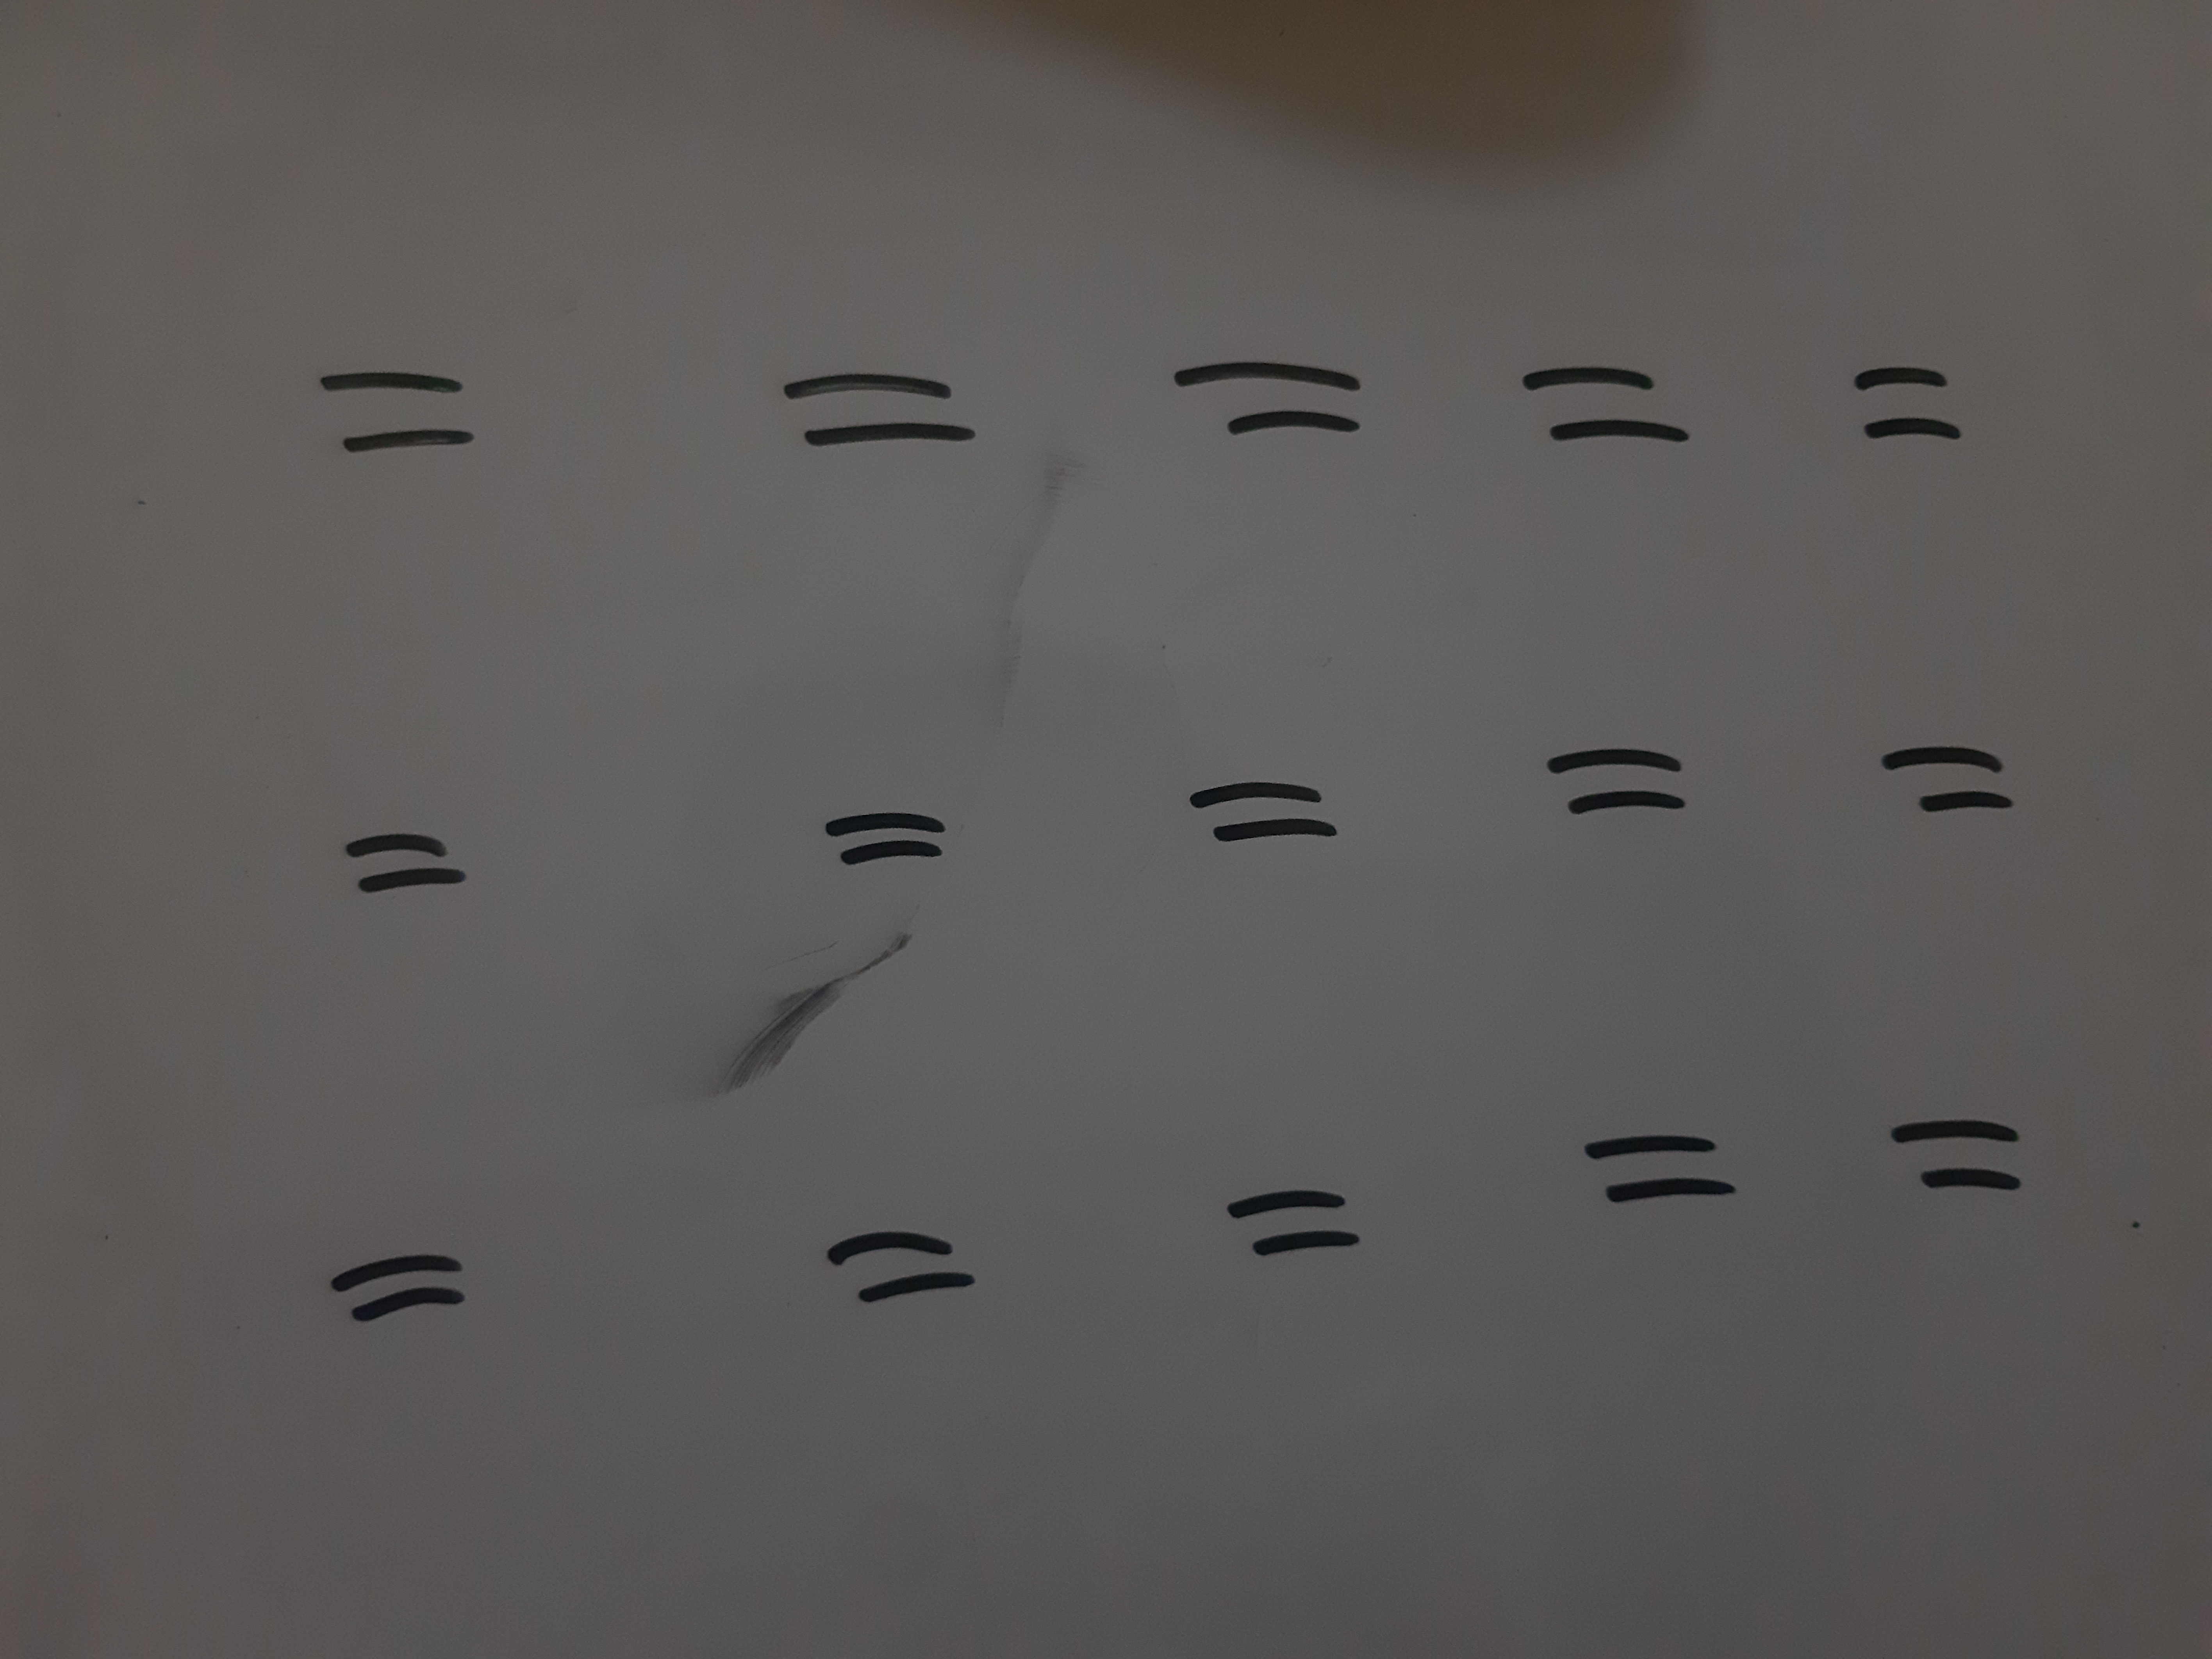
\includegraphics[width=.85\linewidth]{gambar/pengambilan_citra_gelap.jpg}
    \caption{Pengambilan Citra dengan Kondisi \textit{Apperture} Kisaran -1 \textit{Steps.}}
    \label{fig:citragelap}
  \end{subfigure}
  \caption{Pengambilan Citra dengan Variasi Intensitas Cahaya}
  \label{fig:intensitascitrabervariasi}
\end{figure}

\begin{figure}[H]
  \begin{subfigure}{.5\textwidth}
    \centering
    \captionsetup{width=.8\linewidth}
    \includegraphics[width=.85\linewidth]{gambar/pengambilan_citra_depan.jpg}
    \caption{Pengambilan Citra dari Depan}
    \label{fig:citradepan}
  \end{subfigure}%
  \begin{subfigure}{.5\textwidth}
    \centering
    \captionsetup{width=.8\linewidth}
    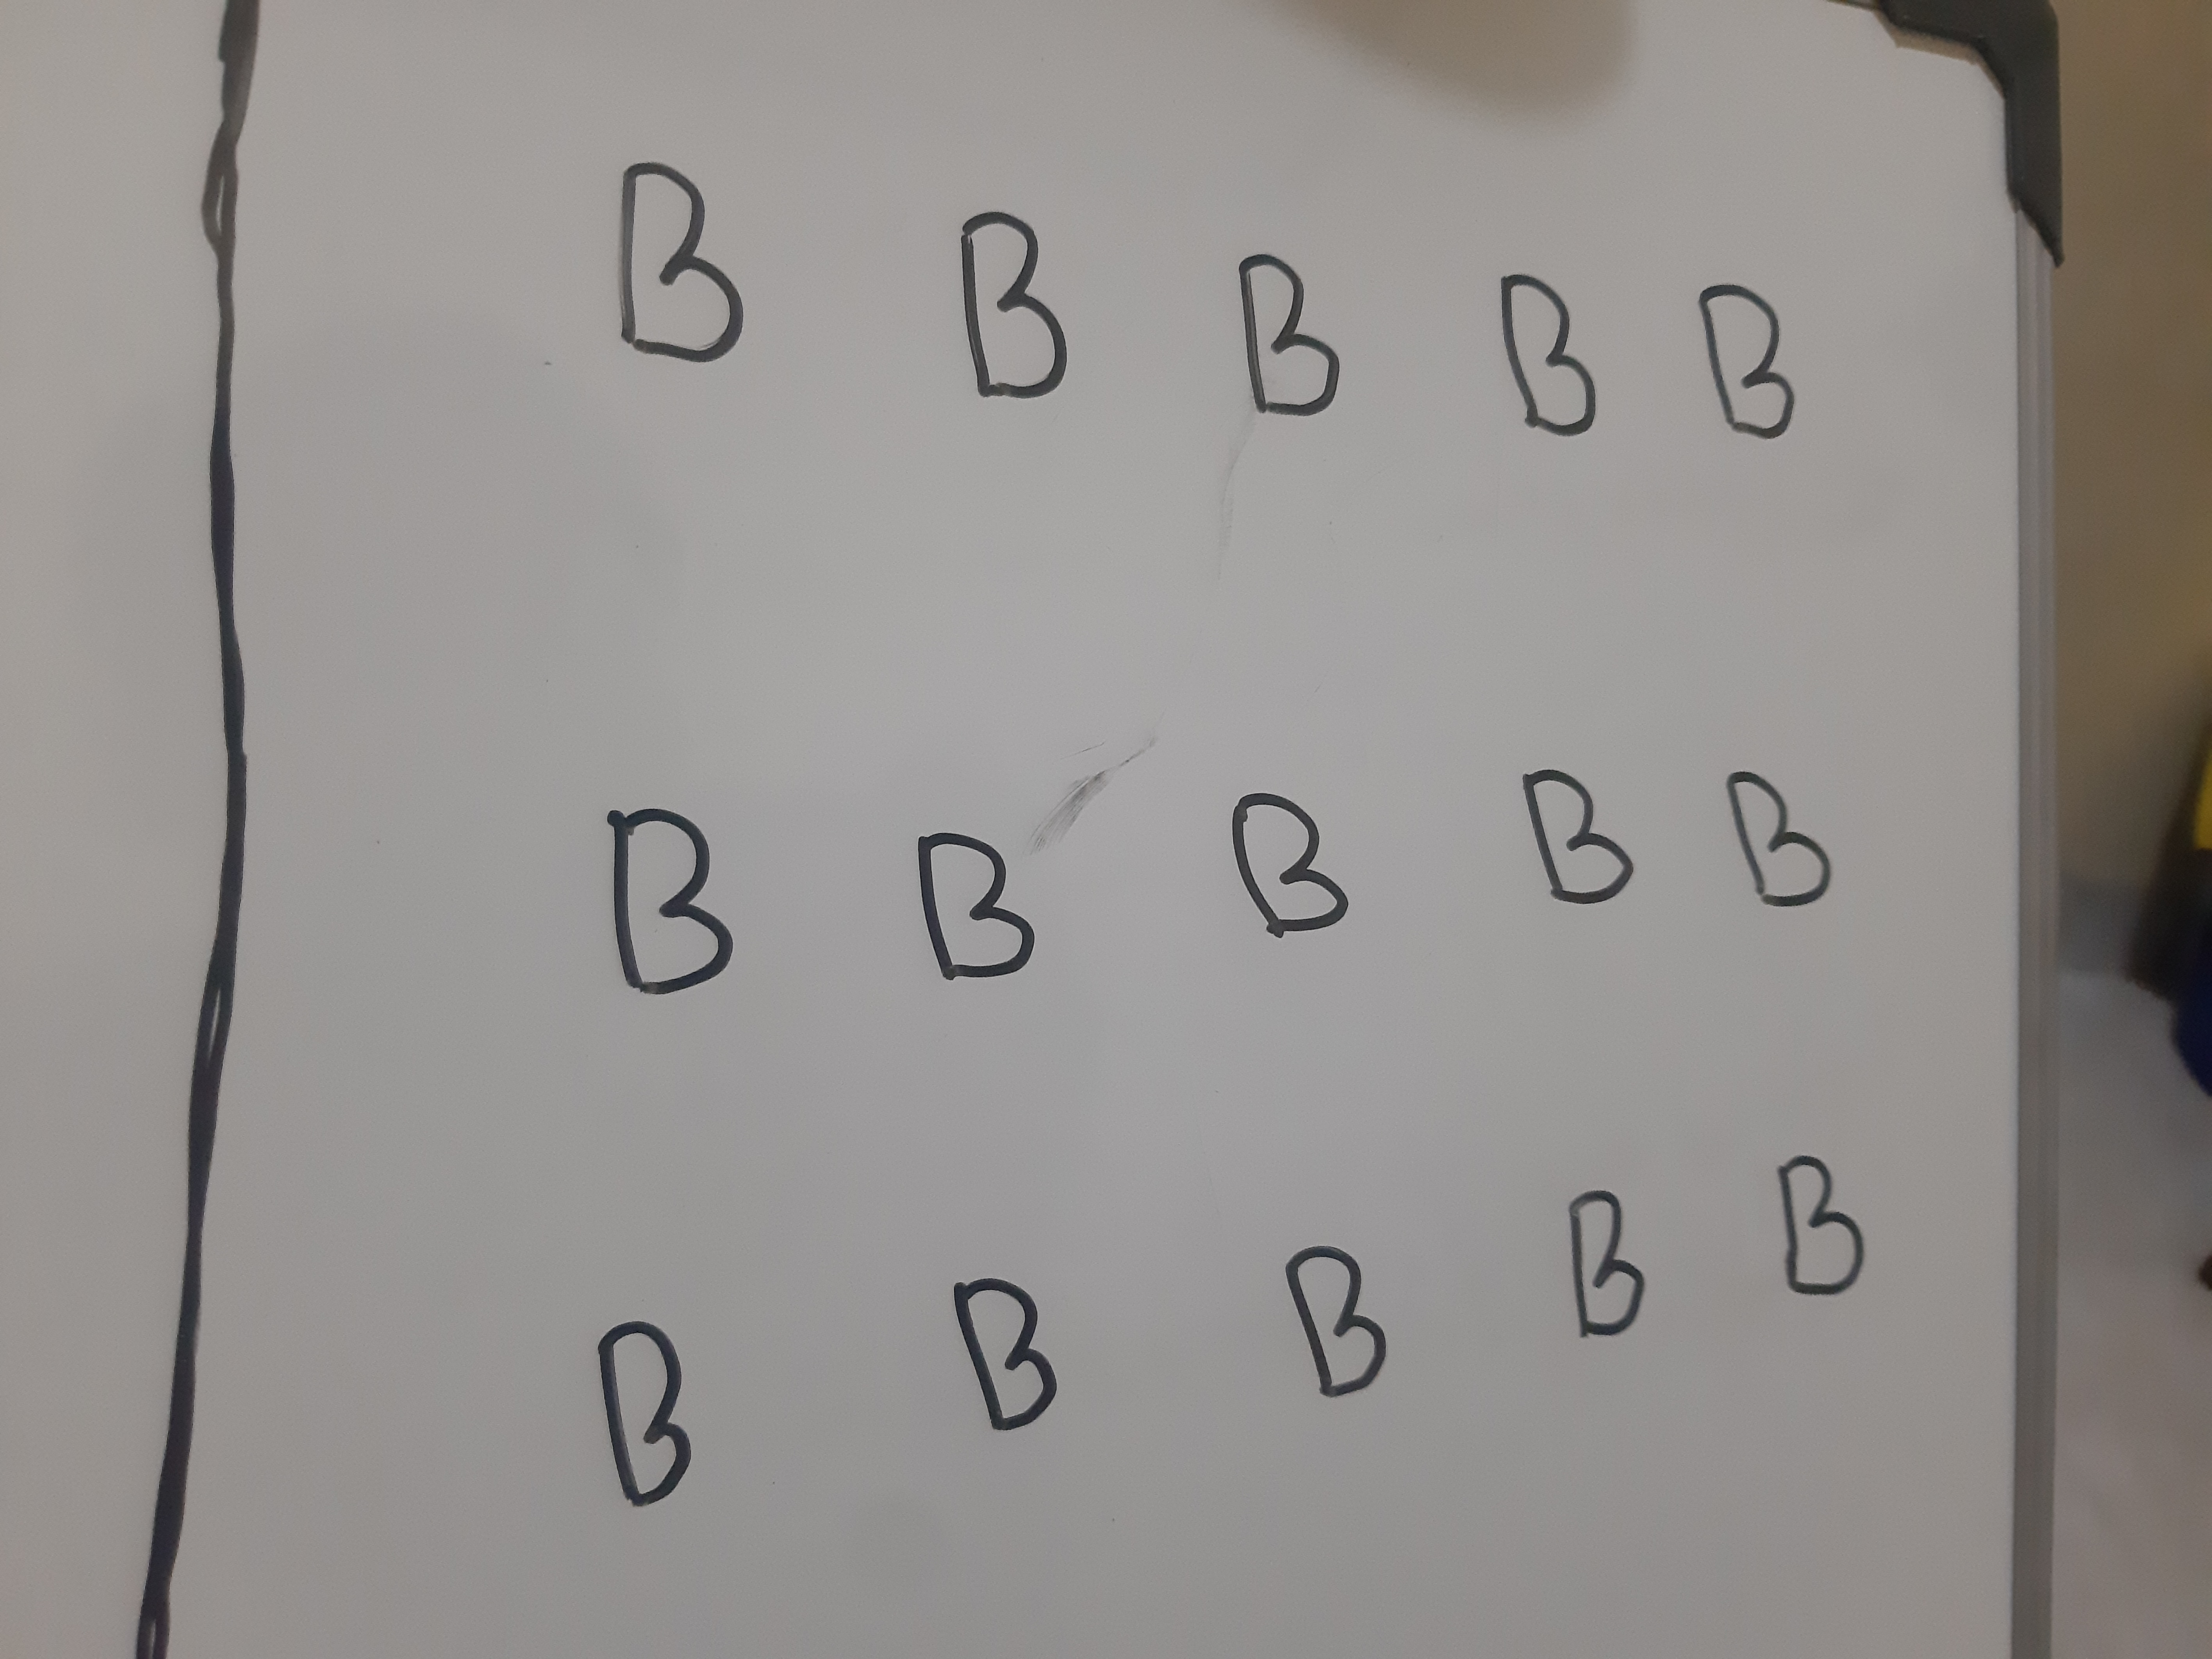
\includegraphics[width=.85\linewidth]{gambar/pengambilan_citra_samping.jpg}
    \caption{Pengambilan Citra dari Samping}
    \label{fig:citrasamping}
  \end{subfigure}
  \caption{Pengambilan Citra dengan Variasi Sudut Pengambilan Gambar}
  \label{fig:pengambilancitrabervariasi}
\end{figure}

Secara spesifik, total persebaran citra pada masing-masing kelas dapat dilihat pada Tabel \ref{tb:jumlahcitratiapkelas} berikut. \par

\begin{center}
  \begin{longtable}[c]{|c|c|c|c|c|}
    \caption{Jumlah Citra Pada Tiap Kelas}
    \label{tb:jumlahcitratiapkelas}\\
  \hline
  \textbf{Kelas} & \textbf{Jumlah Citra} & \textbf{\begin{tabular}[c]{@{}c@{}}\textit{Train Set}\\ (Citra)\end{tabular}} & \textbf{\begin{tabular}[c]{@{}c@{}}\textit{Validation Set}\\ (Citra)\end{tabular}} \\ \hline
  %\endfirsthead
  %
  \endhead
  %
  *             & 50           & 45           & 5           \\ \hline
  =             & 50           & 45           & 5           \\ \hline
  0             & 50           & 45           & 5           \\ \hline
  1             & 50           & 45           & 5           \\ \hline
  2             & 50           & 45           & 5           \\ \hline
  3             & 50           & 45           & 5           \\ \hline
  4             & 50           & 45           & 5           \\ \hline
  5             & 50           & 45           & 5           \\ \hline
  6             & 50           & 45           & 5           \\ \hline
  7             & 50           & 45           & 5           \\ \hline
  8             & 50           & 45           & 5           \\ \hline
  9             & 50           & 45           & 5           \\ \hline
  A             & 50           & 45           & 5           \\ \hline
  B             & 50           & 45           & 5           \\ \hline
  D             & 50           & 45           & 5           \\ \hline
  E             & 50           & 45           & 5           \\ \hline
  G             & 50           & 45           & 5           \\ \hline
  H             & 50           & 45           & 5           \\ \hline
  I             & 50           & 45           & 5           \\ \hline
  J             & 50           & 45           & 5           \\ \hline
  K             & 50           & 45           & 5           \\ \hline
  L             & 50           & 45           & 5           \\ \hline
  M             & 50           & 45           & 5           \\ \hline
  N             & 50           & 45           & 5           \\ \hline
  P             & 50           & 45           & 5           \\ \hline
  R             & 50           & 45           & 5           \\ \hline
  S             & 50           & 45           & 5           \\ \hline
  T             & 50           & 45           & 5           \\ \hline
  U             & 50           & 45           & 5           \\ \hline
  V             & 50           & 45           & 5           \\ \hline
  \textit{null} & 26           & 26           & 0           \\ \hline
  \end{longtable}
\end{center}
  
\subsubsection{Hasil Proses Pelabelan Dataset}
\label{subsubsec:hasilpelabelan}

Proses pelabelan dilakukan dengan memberikan \textit{bounding box} pada tiap-tiap citra yang telah dikumpulkan pada tahap sebelumnya. Pada proses \textit{bounding box,} tiap-tiap citra yang termasuk sebagai objek dari tiap kelas dianotasi sehingga seluruh bagian objeknya berada didalam anotasi dan diberi label sesuai dengan kelas objeknya. Anotasi pada proses pelabelan ini menggunakan anotasi berbentuk segiempat. Setelah proses pelabelan dilakukan maka \textit{output} yang dihasilkan pada tiap citra yang diolah yaitu sebuah file citra yang sudah di-\textit{pre-process} dan sebuah file txt berisi titik koordinat dari tiap objek yang ada pada sebuah citra tersebut. Adapun proses pelabelan dataset dapat dilihat pada Gambar \ref{fig:labellingroboflow}. 

\begin{figure}[H]
  \centering
  \includegraphics[scale=0.39]{gambar/labelling.png}
  \caption{Proses Pelabelan menggunakan Roboflow}
  \label{fig:labellingroboflow}
\end{figure}

Setelah dilakukan proses pelabelan, \textit{output} yang dihasilkan yaitu gambar yang memiliki \textit{bounding box}, dan apabila di-\textit{export} maka dataset hasil pelabelan terdiri dari 2 file yaitu file citra itu sendiri dan juga file txt yang berisi koordinat \textit{bounding box} yang ada pada suatu citra tersebut. Adapun total persebaran anotasi \textit{bounding box} pada masing-masing kelas dapat dilihat pada Tabel \ref{tb:anotasitiapkelas} berikut. 


\begin{center}
  \begin{longtable}[c]{|c|c|c|c|c|}
  \caption{Jumlah Anotasi Tiap Kelas}
  \label{tb:anotasitiapkelas}\\
  \hline
  \textbf{Kelas} & \textbf{Jumlah Anotasi} \\ \hline
  %\endfirsthead
  %
  \endhead
  %
  *             & 750             \\ \hline
  =             & 750             \\ \hline
  0             & 750             \\ \hline
  1             & 750             \\ \hline
  2             & 750             \\ \hline
  3             & 750             \\ \hline
  4             & 750             \\ \hline
  5             & 750             \\ \hline
  6             & 750             \\ \hline
  7             & 750             \\ \hline
  8             & 750             \\ \hline
  9             & 750             \\ \hline
  A             & 756             \\ \hline
  B             & 750             \\ \hline
  D             & 751             \\ \hline
  E             & 750             \\ \hline
  G             & 750             \\ \hline
  H             & 750             \\ \hline
  I             & 750             \\ \hline
  J             & 750             \\ \hline
  K             & 750             \\ \hline
  L             & 750             \\ \hline
  M             & 750             \\ \hline
  N             & 750             \\ \hline
  P             & 750             \\ \hline
  R             & 750             \\ \hline
  S             & 750             \\ \hline
  T             & 750             \\ \hline
  U             & 751             \\ \hline
  V             & 750             \\ \hline
  \end{longtable}
\end{center}

\subsubsection{Hasil \textit{Image Pre-Processing}}
\label{subsubsec:hasilpreprocess}

Pada tahap \textit{pre-process}, citra yang telah diberi label selanjutnya dilakukan \textit{pre-process} tertentu. Tahapan \textit{pre-process} bertujuan untuk mengurangi waktu \textit{training} dan meningkatkan performa. Secara ringkas, tahapan \textit{pre-process} yang dilakukan yaitu seperti pada Tabel \ref*{tb:checklistpreprocess}. Secara spesifik, pada tahapan \textit{pre-process} melakukan proses transformasi citra tertentu yaitu:
\begin{enumerate}[nolistsep]
  \item \textit{\textbf{Auto Orient.} Auto Orient} dilakukan untuk agar citra yang ditampilkan orientasinya sesuai dengan ketika diambil pada pengambilan awal.
  \item \textit{\textbf{Resize.} Resize} dilakukan untuk mengubah dimensi citra menjadi lebih kecil. Citra diubah dengan pengaturan \textit{stretch} sehingga tiap citra yang sebelumnya tidak memiliki dimensi ukuran 416x416 diregangkan ukurannya menjadi ukuran 416x416.
  \item \textit{\textbf{Grayscale.} \textnormal{Proses} Grayscale} bertujuan untuk memperkecil variasi warna gambar khususnya objek yang dibuat dengan spidol sehingga proses \textit{train} menjadi lebih cepat. Hasil dari proses \textit{grayscale} seperti pada Gambar \ref{fig:grayscallingdataset}.
    \begin{figure}[H]
      \centering
      \includegraphics[scale=0.33]{gambar/grayscalling.png}
      \caption{Gambar Sebelum dan Setelah Proses \textit{Grayscalling}}
      \label{fig:grayscallingdataset}
    \end{figure}
  \item \textit{\textbf{Contrast.} Contrast} dilakukan agar tepian-tepian yang ada pada citra dapat lebih terlihat perbedaannya. Jenis \textit{contrast} yang dilakukan yaitu \textit{contrast stretching. Contrast stretching} adalah teknik transformasi citra yaitu meningkatkan kontras dalam citra dengan melakukan \textit{stretch} atau peregangan rentang intensitas nilai untuk menjangkau rentang nilai yang diinginkan.
  % \item \textit{\textbf{Filter Null.}}
  % \item \textit{\textbf{Blur.}}
  % \item \textit{\textbf{Noise.}}
  % \item \textit{\textbf{Bounding Box Rotation.}}
\end{enumerate}

\subsection{Hasil \textit{Training} dan \textit{Validation}}
\label{subsec:hasiltrainvaldata}

% halooooo, chesia was here
Pada tugas akhir ini, \textit{pretrained weight} yang digunakan yaitu YOLOv5s. \textit{pretrained weight} YOLOv5s dipilih karena jika dibandingkan dengan versi lain seperti YOLOv5m, YOLOv5l memiliki hasil yang relatif lebih rendah, namun dengan menggunakan YOLOv5s hasil dapat didapatkan lebih cepat dan juga cocok jika di-\textit{deploy} pada perangkat kecil seperti perangkat \textit{mobile}. Proses \textit{training} data dilakukan setelah proses pengumpulan citra, proses pelabelan, dan pre-proses gambar selesai dilaksanakan. Adapun hasil dari proses \textit{training} ini yaitu berupa model dan detail data angka pada tiap proses pengulangan  (epochs). Detail spesifikasi laptop yang digunakan dalam melakukan proses \textit{training} yaitu sesuai pada Tabel \ref{tb:spesifikasilaptop}, sedangkan detail hyperparameter dan konfigurasi yang digunakan dapat dilihat pada Tabel \ref*{tb:parametertrain} berikut. \par 

\begin{table}[H]
  \caption{Detail Hyperparameter yang Digunakan}
  \label{tb:parametertrain}
  \begin{center}
    \begin{tabularx}{0.5\textwidth}{|X<{\centering}|X<{\centering}|}
      \hline
      % \textbf{Parameter}                       & \textbf{Nilai}          \\ \hline
      \textit{Weights}                         & YOLOv5s                 \\ \hline
      \textit{Class Number}                    & 30                      \\ \hline
      Epochs                                   & 300                      \\ \hline
      \textit{Batch-Size}                      & 16                      \\ \hline
      \textit{Image Size}                      & 416                     \\ \hline
      \textit{Learning Rate}                   & 0.01                    \\ \hline
      \textit{Optimizer}                       & SGD                     \\ \hline
    \end{tabularx}
  \end{center}  
\end{table}

Proses \textit{training} dilakukan menggunakan dataset \textit{training set}. Setelah dilakukan proses \textit{train} dengan konfigurasi sesuai pada Tabel \ref*{tb:parametertrain}, selanjutnya dilakukan proses \textit{validation.} Pada tahapan \textit{validation} yaitu model diuji dengan menggunakan dataset \textit{validation set} dan kemudian didapatkan hasil \textit{train} berupa \textit{loss, precision, recall, \textnormal{dan} mAP} sesuai Gambar \ref*{fig:trainresult} yaitu: \par

\begin{figure}[H]
  \centering
  \includegraphics[scale=0.5]{gambar/train_results.png}
  \caption{Hasil Training menggunakan YOLOv5s}
  \label{fig:trainresult}
\end{figure}

Serta didapatkan detail dari akurasi masing-masing huruf yaitu sebagai berikut: \par

\begin{center}
  \begin{longtable}[c]{|c|c|c|c|c|c|c|}
    \caption{Hasil \textit{Training} Perkelas}
    \label{tb:trainperkelas}\\
    \hline
    \textbf{Kelas} & \textbf{Gambar} & \textbf{Jumlah Label} & \textbf{P} & \textbf{R} & \textbf{mAP 0.5} & \textbf{mAP 0.5 0.95} \\ \hline
    %\endfirsthead
    %
    \endhead
    %
    *              & 5                          & 105                   & 0.999      & 1          & 0.995            & 0.875                 \\ \hline
    =              & 5                          & 105                   & 0.999      & 1          & 0.995            & 0.907                 \\ \hline
    0              & 5                          & 105                   & 0.999      & 1          & 0.995            & 0.773                 \\ \hline
    1              & 5                          & 105                   & 0.999      & 1          & 0.995            & 0.83                  \\ \hline
    2              & 5                          & 165                   & 1          & 1          & 0.995            & 0.849                 \\ \hline
    3              & 5                          & 165                   & 0.999      & 1          & 0.995            & 0.854                 \\ \hline
    4              & 5                          & 105                   & 0.999      & 1          & 0.995            & 0.895                 \\ \hline
    5              & 5                          & 105                   & 0.999      & 1          & 0.995            & 0.872                 \\ \hline
    6              & 5                          & 105                   & 0.999      & 1          & 0.995            & 0.862                 \\ \hline
    7              & 5                          & 105                   & 1          & 1          & 0.995            & 0.875                 \\ \hline
    8              & 5                          & 105                   & 0.999      & 1          & 0.995            & 0.845                 \\ \hline
    9              & 5                          & 105                   & 0.999      & 1          & 0.995            & 0.859                 \\ \hline
    A              & 5                          & 105                   & 0.999      & 1          & 0.995            & 0.875                 \\ \hline
    B              & 5                          & 105                   & 0.999      & 1          & 0.995            & 0.907                 \\ \hline
    D              & 5                          & 105                   & 0.999      & 1          & 0.995            & 0.83                  \\ \hline
    E              & 5                          & 165                   & 1          & 1          & 0.995            & 0.849                 \\ \hline
    G              & 5                          & 105                   & 0.999      & 1          & 0.995            & 0.895                 \\ \hline
    H              & 5                          & 105                   & 0.999      & 1          & 0.995            & 0.872                 \\ \hline
    I              & 5                          & 105                   & 0.999      & 1          & 0.995            & 0.862                 \\ \hline
    J              & 5                          & 105                   & 1          & 1          & 0.995            & 0.875                 \\ \hline
    K              & 5                          & 105                   & 0.999      & 1          & 0.995            & 0.845                 \\ \hline
    L              & 5                          & 105                   & 0.999      & 1          & 0.995            & 0.859                 \\ \hline
    M              & 5                          & 165                   & 1          & 1          & 0.995            & 0.832                 \\ \hline
    N              & 5                          & 165                   & 1          & 1          & 0.995            & 0.799                 \\ \hline
    P              & 5                          & 105                   & 1          & 1          & 0.995            & 0.824                 \\ \hline
    R              & 5                          & 105                   & 1          & 1          & 0.995            & 0.844                 \\ \hline
    S              & 5                          & 105                   & 1          & 1          & 0.995            & 0.893                 \\ \hline
    T              & 5                          & 105                   & 0.999      & 1          & 0.995            & 0.874                 \\ \hline
    U              & 5                          & 165                   & 0.999      & 1          & 0.995            & 0.844                 \\ \hline
    V              & 5                          & 165                   & 0.999      & 1          & 0.995            & 0.867                 \\ \hline
  \end{longtable}
\end{center}

Setelah didapatkan hasil model, dilakukan proses validasi untuk menentukan apakah model tersebut sudah cukup akurat atau masih membutuhkan perbaikan. Pada proses validasi, terdapat matriks yang umum digunakan untuk melakukan validasi model yaitu \textit{evaluation metrics.} Menggunakan \textit{confusion matrix,} didapatkan hasil yaitu seperti pada gambar \ref*{fig:confusionmetrics} berikut.

\begin{figure}[H]
  \centering
  \includegraphics[scale=0.5]{gambar/confusion_matrix.png}
  \caption{Hasil \textit{Evaluation Metrics} Menggunakan \textit{Confusion Matrix}}
  \label{fig:confusionmetrics}
\end{figure}

Adapun hasil percobaan pembacaan menggunakan data diluar dataset didapatkan hasil sesuai Gambar \ref*{fig:detectbaru} berikut.

\begin{figure}[H]
  \centering
  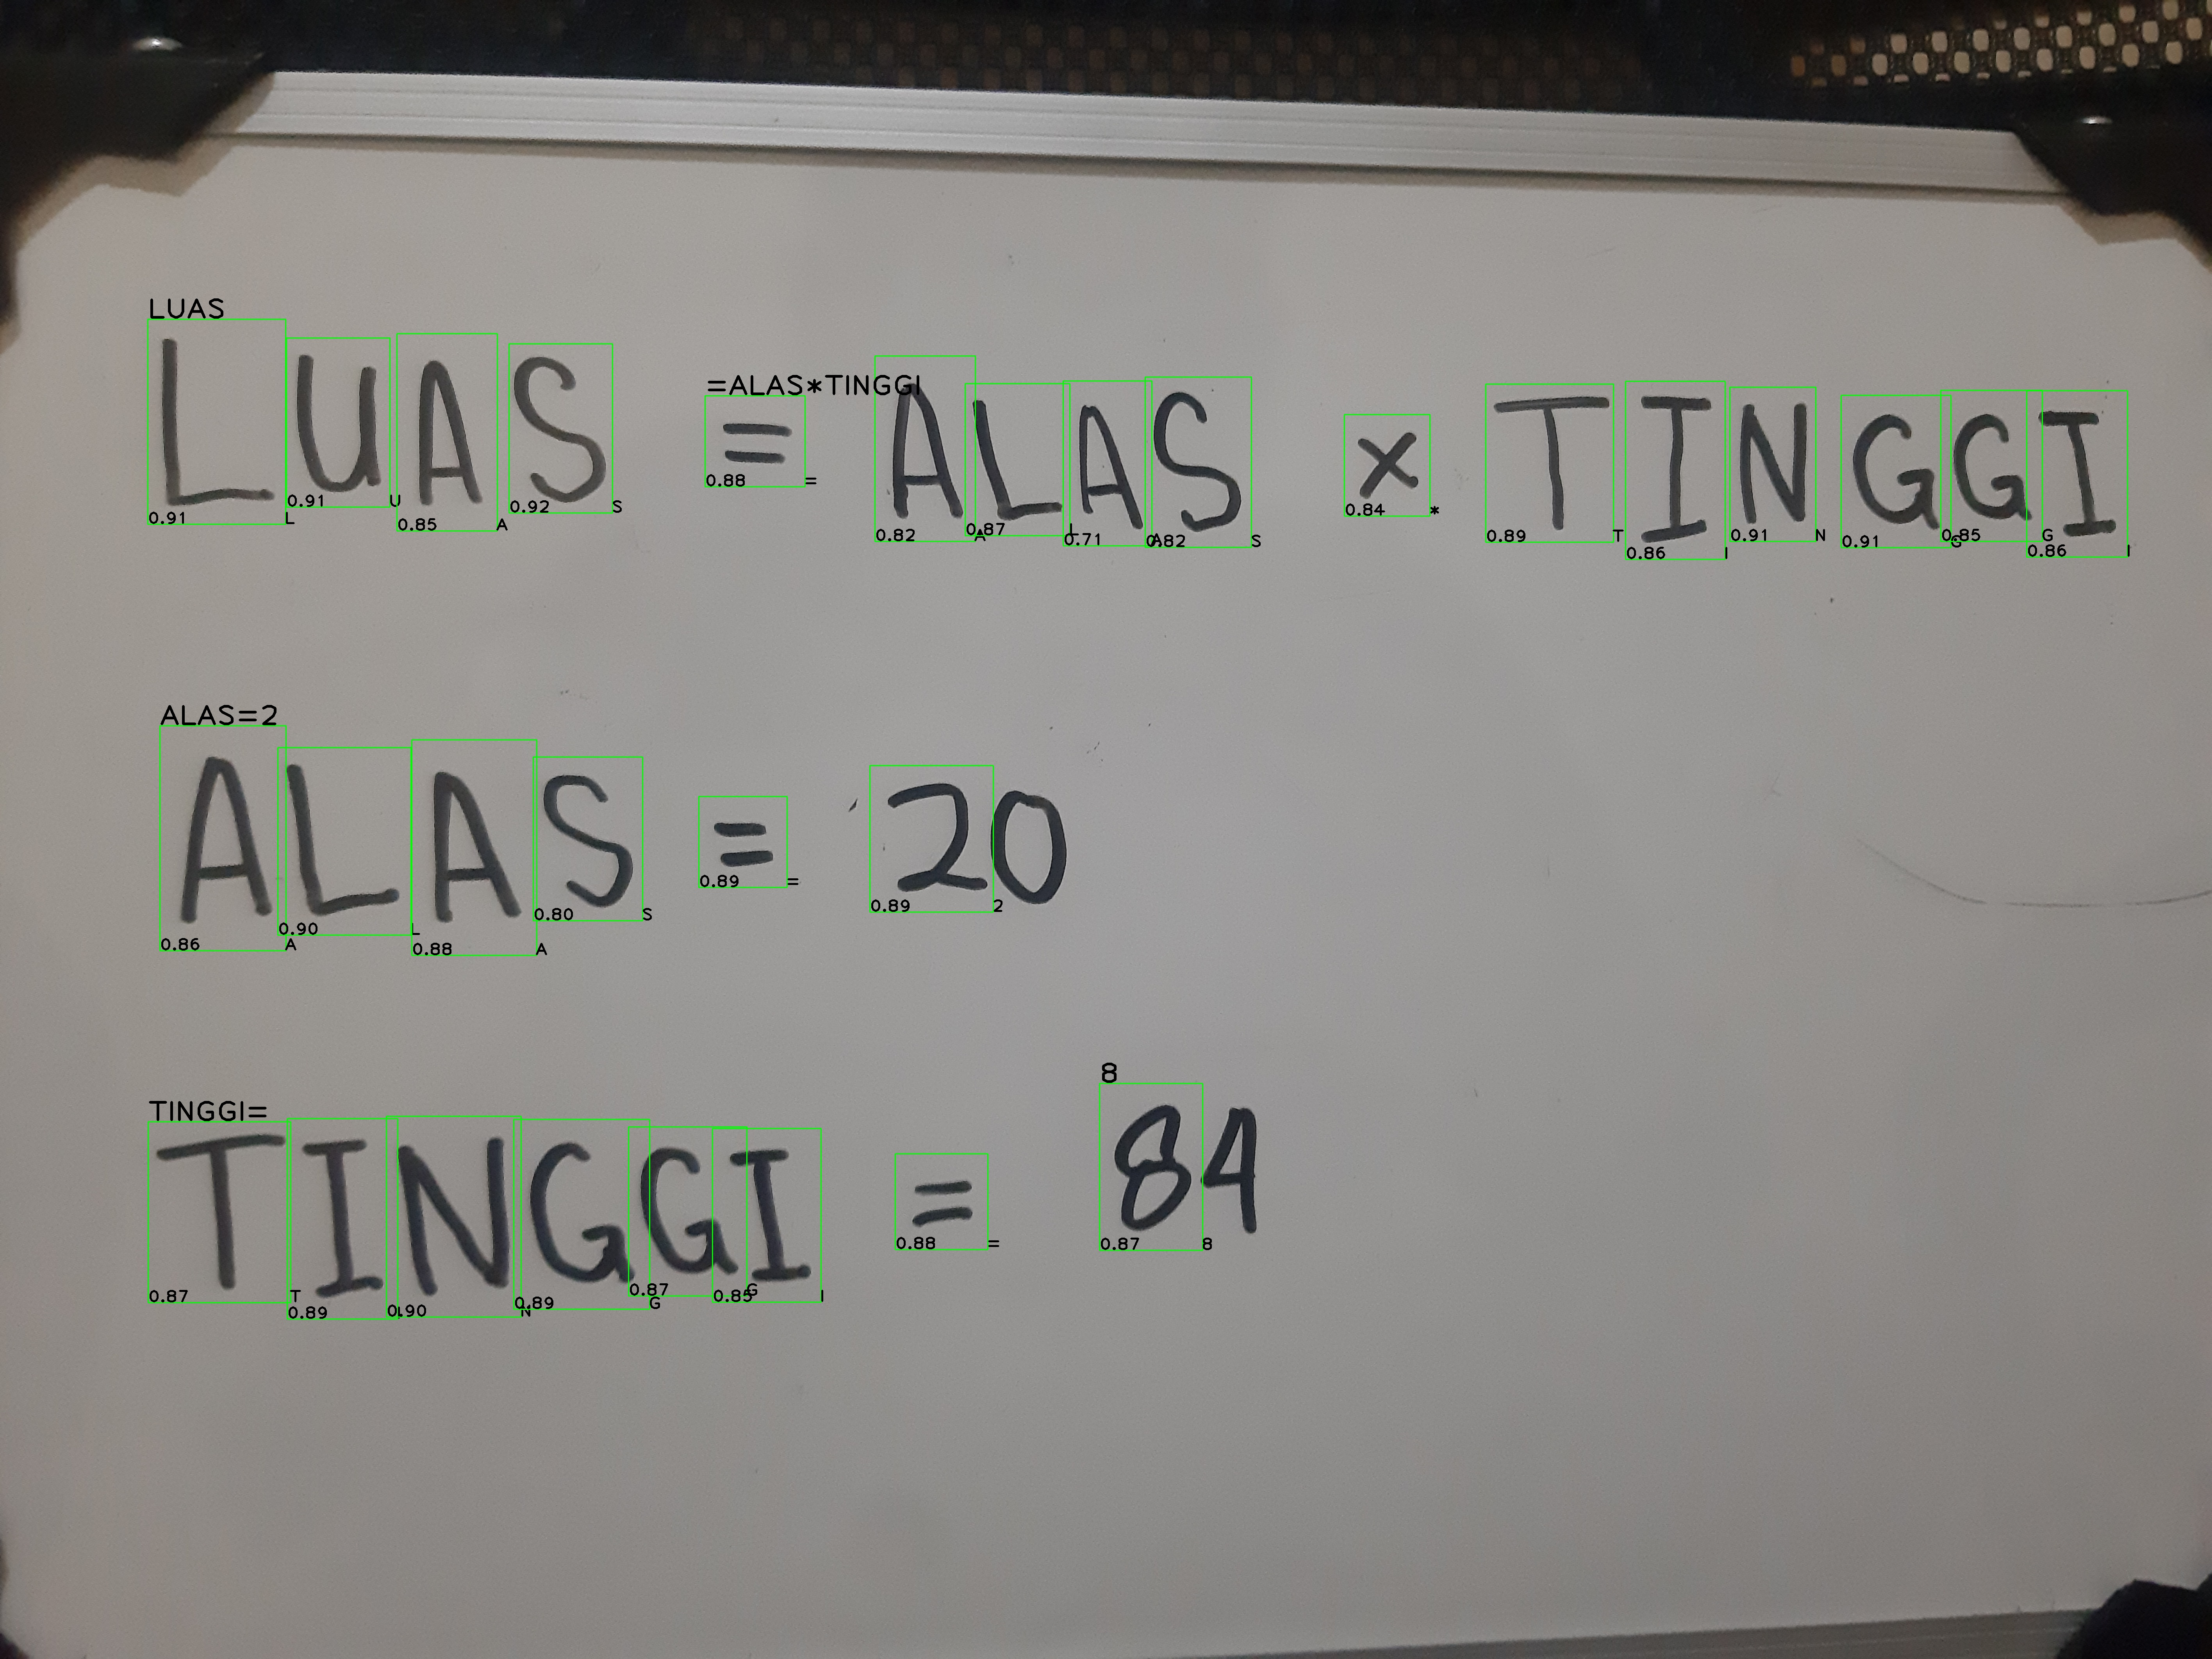
\includegraphics[scale=0.05]{gambar/detectdiluardataset.jpg}
  \caption{Hasil Deteksi Menggunakan Data Responden}
  \label{fig:detectbaru}
\end{figure}


Pada tahapan \textit{training \textnormal{dan} validation} telah dilakukan proses \textit{training} model menggunakan \textit{pretrained weight} YOLOv5n, YOLOv5s, dan YOLOv5m. Menggunakan jumlah dataset yang sama, pemrosesan citra yang sama, serta konfigurasi \textit{hyperparameter} yang sama, didapatkan hasil bahwa semakin kompleks layer dan proses yang dilakukan dalam pembangunan model maka hasil yang didapatkan akan semakin baik, namun waktu yang dibutuhkan untuk membangun model tersebut juga menjadi lebih panjang.

% Pada proses pengujian didapatkan hasil bahwa model 
% sementara masih \textit{\textbf{overfit}} dikarenakan walaupun pada hasil \textit{training} memiliki akurasi cukup tinggi, namun ketika dilakukan uji coba menggunakan gambar diluar dataset yag telah disediakan hasilnya masih berantakan. \par
% sudah dapat berfungsi seperti ditunjukkan pada gambar berikut. \par

\subsection{Hasil Pembuatan Algoritma Konversi Gambar menjadi Teks}
\label{subsec:hasilmembangunmodel}

Setelah didapatkan model hasil \textit{training} dan sudah memiliki akurasi cukup untuk dapat melakukan deteksi dengan baik, selanjutnya dilakukan proses pembangunan model konversi gambar menjadi teks. Proses pembangunan model konversi gambar menjadi teks ini diprogram dengan menggunakan bahasa Python. Adapun alur model konversi gambar menjadi teks dimlai dari pengguna melakukan input gambar yang ingin dikonversi kedalam program. Setelah gambar dimasukkan kedalam program, gambar tersebut diubah ukurannya menjadi 416x416, dengan menggunakan \textit{library} opencv. \par

Setelah ukuran gambar disesuaikan, selanjutnya menentukan koordinat seluruh \textit{bounding box} yang tersedia dan terbaca dengan menggunakan model yang telah di\textit{-train} sebelumnya. Setelah koordinat \textit{bounding box} didapat, seluruh \textit{bounding box} yang terbaca dikelompokan berdasarkan jarak antara \textit{bounding box} pertama dengan \textit{bounding box} selanjutnya, jika jarak antaranya memenuhi \textit{threshold} tertentu, maka akan dikelompokan kedalam sebuah List yang sama, dan jika tidak memenuhi maka akan diletakan pada kelompok List berikutnya. Adapun \textit{threshold} yang digunakan yaitu pada koordinat X sebesar lebar X \textit{bounding-box} paling pertama dan koordinat Y sebesar lebar Y \textit{bounding-box} paling pertama. Prioritas pengelompokan diatur berdasarkan koordinat Y terlebih dahulu kemudian dilanjutkan dengan koordinat X, hal ini bertujuan agar teks yang ditampilkan berurutan dari baris paling atas lalu bergerak kearah X+ (kanan), dan dilanjut pada baris kedua dan seterusnya. \par

Ketika seluruh \textit{bounding box} telah disortir dan dikelompokkan berdasarkan koordinat X dan Y, proses selanjutnya yaitu seluruh \textit{bounding box} dikembalikan nilainya. Adapun nilai kembalian yang didapatkan dapat ditampilkan dalam gambar langsung ataupun dalam bentuk String. 

\section{Skenario Pengujian}
\label{sec:skenariopengujian}

Pada sub ini dilakukan berbagai skenario pengujian guna mengetahui tingkat kesalahan dan membuka potensi pengembangan penelitian dimasa mendatang serta menarik kesimpulan secara keseluruhan. Secara spesifik, skenario pengujian yang dilakukan yaitu sebagai berikut: \par

\subsection{Pengujian Menggunakan \textit{Pretrained Weight} Model yang Bervariasi}
\label{subsec:pengujianpretrainedweight}

Pada pengujian pertama yaitu pengujian menggunakan \textit{pretrained weight} model yang bervariasi. Tujuan dari pengujian ini yaitu untuk membandingkan performa dan hasil yang didapat dengan performa dan hasil yang didapat dari model lain. Pada pengujian dengan \textit{pretrained weight} model ini menggunakan model YOLOv5n, YOLOv5s, dan YOLOv5m. Pengujian dilaksanakan dengan cara melakukan proses \textit{train} dengan konfigurasi serupa antar parameter dan \textit{hyperparameter} seperti pada Tabel \ref*{tb:parametertrain}. Dari pengujian pertama ini didapatkan hasil seperti pada Tabel \ref*{tb:variasipretrainedweight} berikut. \par

\begin{center}
  \begin{longtable}[c]{|c|c|c|c|}
    \caption{Pengujian dengan Variasi Pretrained Weight }
    \label{tb:variasipretrainedweight}\\
    \hline
    \textbf{}                                                                          & \textbf{YOLOv5n} & \textbf{YOLOv5s} & \textbf{YOLOv5m} \\ \hline
    %\endfirsthead
    %
    \endhead
    %
    \textit{\textbf{\begin{tabular}[c]{@{}c@{}}Training\\ Box Loss\end{tabular}}}      & 0.020503           & 0.019025         & \textbf{0.017891}          \\ \hline
    \textit{\textbf{\begin{tabular}[c]{@{}c@{}}Training\\ Object Loss\end{tabular}}}   & 0.031525           & 0.02999          & \textbf{0.029318}          \\ \hline
    \textit{\textbf{\begin{tabular}[c]{@{}c@{}}Training\\ Class Loss\end{tabular}}}    & 0.0024306          & 0.0014572        & \textbf{0.0010953}         \\ \hline
    \textit{\textbf{\begin{tabular}[c]{@{}c@{}}Validation\\ Box Loss\end{tabular}}}    & \textbf{0.015289}  & 0.015308         & 0.014543                   \\ \hline
    \textit{\textbf{\begin{tabular}[c]{@{}c@{}}Validation\\ Object Loss\end{tabular}}} & 0.022269           & 0.022385         & \textbf{0.022056}          \\ \hline
    \textit{\textbf{\begin{tabular}[c]{@{}c@{}}Validation\\ Class Loss\end{tabular}}}  & 0.00054263         & 0.00036628       & \textbf{0.00034182}        \\ \hline
    \multicolumn{1}{|l|}{\textit{\textbf{Precision}}}                                  & \textbf{0.99899}   & 0.99881          & 0.99887                    \\ \hline
    \multicolumn{1}{|l|}{\textit{\textbf{Recall}}}                                     & 0.99905            & 0.99984          & \textbf{0.99987}           \\ \hline
    \multicolumn{1}{|l|}{\textbf{mAP}}                                                 & 0.83331            & 0.82873          & \textbf{0.84223}           \\ \hline
  \end{longtable}
\end{center}

% Dari tabel berikut dapat terlihat bahwa nilai \textit{loss} terendah yaitu pada model (...) dan nilai precision tertinggi yaitu pada model (...).

\subsection{Pengujian Menggunakan \textit{Pretrained Weight} YOLOv5n}
\label{subsec:pengujianyolov5n}

Pada pengujian menggunakan \textit{pretrained weight} model YOLOv5n, dilakukan validasi terhadap hasil model yang telah dibuat menggunakan \textit{pretrained weight} model YOLOv5n sehingga didapatkan hasil validasi sesuai Gambar \ref*{fig:trainresultyolov5n} serta hasil \textit{train} sesuai Tabel \ref*{tb:valresultyolov5n} berikut. \par

\begin{figure}[H]
  \centering
  \includegraphics[scale=0.5]{gambar/yolov5n/train_results.png}
  \caption{Hasil \textit{Training} menggunakan model YOLOv5n}
  \label{fig:trainresultyolov5n}
\end{figure}

\begin{center}
  \begin{longtable}[c]{|c|c|c|c|c|c|}
    \caption{Hasil Validasi menggunakan model YOLOv5n}
    \label{tb:valresultyolov5n}\\
    \hline
    \textbf{Kelas} & \textbf{Citra} & \textbf{Label} & \textbf{Precision} & \textbf{Recall} & \textbf{mAP} \\ \hline
    \endhead
    %
    *      & 5      & 75     & 0.999      & 1      & 0.869    \\ \hline
    =      & 5      & 75     & 0.999      & 1      & 0.756    \\ \hline
    0      & 5      & 75     & 0.999      & 1      & 0.816    \\ \hline
    1      & 5      & 75     & 1          & 0.993  & 0.79     \\ \hline
    2      & 5      & 75     & 0.999      & 1      & 0.814    \\ \hline
    3      & 5      & 75     & 0.999      & 1      & 0.866    \\ \hline
    4      & 5      & 75     & 0.999      & 1      & 0.819    \\ \hline
    5      & 5      & 75     & 0.999      & 1      & 0.841    \\ \hline
    6      & 5      & 75     & 0.999      & 1      & 0.839    \\ \hline
    7      & 5      & 75     & 0.999      & 1      & 0.778    \\ \hline
    8      & 5      & 75     & 1          & 1      & 0.784    \\ \hline
    9      & 5      & 75     & 0.999      & 1      & 0.813    \\ \hline
    A      & 5      & 75     & 0.999      & 1      & 0.792    \\ \hline
    B      & 5      & 75     & 0.999      & 1      & 0.825    \\ \hline
    D      & 5      & 75     & 0.999      & 1      & 0.844    \\ \hline
    E      & 5      & 75     & 1          & 1      & 0.862    \\ \hline
    G      & 5      & 75     & 0.999      & 1      & 0.845    \\ \hline
    H      & 5      & 75     & 0.998      & 1      & 0.887    \\ \hline
    I      & 5      & 75     & 0.999      & 1      & 0.861    \\ \hline
    J      & 5      & 75     & 0.974      & 1      & 0.784    \\ \hline
    K      & 5      & 75     & 0.999      & 1      & 0.74     \\ \hline
    L      & 5      & 75     & 1          & 1      & 0.853    \\ \hline
    M      & 5      & 75     & 0.999      & 1      & 0.831    \\ \hline
    N      & 5      & 75     & 0.999      & 1      & 0.857    \\ \hline
    P      & 5      & 75     & 0.999      & 1      & 0.868    \\ \hline
    R      & 5      & 75     & 0.999      & 1      & 0.848    \\ \hline
    S      & 5      & 75     & 0.999      & 1      & 0.837    \\ \hline
    T      & 5      & 75     & 0.999      & 1      & 0.85     \\ \hline
    U      & 5      & 75     & 0.999      & 1      & 0.849    \\ \hline
    V      & 5      & 75     & 0.999      & 1      & 0.858    \\ \hline 
  \end{longtable}
\end{center}

Selanjutnya, model yang telah dibuat dan didapatkan hasilnya kemudian dilakukan serangkaian skenario pengujian. Skenario pengujian yang dilakukan yaitu model akan diuji untuk melakukan pembacaan citra dari tulisan tangan oleh beberapa responden berbeda, yang pada tiap responden dilakukan pengujian berdasarkan jarak pengambilan citra serta tingkat pencahayaan dalam pengambilan citra. Pada jarak pengambilan citra, citra diambil dengan kondisi jarak pengambilan 20cm, 30cm, dan 40cm. Sedangkan pada pencahayaan dalam pengambilan citra, citra diambil dengan kondisi pencahayaan normal dan dengan konfigurasi kamera \textit{apperture} -1.0 \textit{steps.} Secara spesifik, pengujian yang akan dilakukan dapat dilihat pada sub berikut.

\subsubsection{Skenario Pengujian Menggunakan Data Citra dari Responden 1}
\label{subsubsec:nskenarioresponden1}

Pada pengujian pembacaan citra dari responden 1, data yang akan diuji dibagi menjadi skenario berdasarkan jarak pengambilan citra dan tingkat pencahayaan citra. Adapun hasil pembacaan yaitu didapatkan hasil yaitu seperti pada Gambar \ref*{fig:nr1citra20cm}, Gambar \ref*{fig:nr1citra30cm}, dan Gambar \ref*{fig:nr1citra40cm}.

% 20cm
\begin{figure}[H]
  \begin{subfigure}{.5\textwidth}
    \centering
    \captionsetup{width=.8\linewidth}
    \includegraphics[width=.8\linewidth]{gambar/yolov5n/responden1/dinda20cm00-result.jpg}
    \caption{Responden 1. Pengambilan Citra Jarak 20 Cm. Pencahayaan Normal}
    \label{fig:nr1tcitra20cm}
  \end{subfigure}%
  \begin{subfigure}{.5\textwidth}
    \centering
    \captionsetup{width=.8\linewidth}
    \includegraphics[width=.8\linewidth]{gambar/yolov5n/responden1/dinda20cm10-result.jpg}
    \caption{Responden 1. Pengambilan Citra Jarak 20 Cm. Pencahayaan Gelap}
    \label{fig:nr1gcitra20cm}
  \end{subfigure}
  \caption{YOLOv5n. Responden 1. Pengambilan Citra Jarak 20 Cm}
  \label{fig:nr1citra20cm}
\end{figure}

% 30cm
\begin{figure}[H]
  \begin{subfigure}{.5\textwidth}
    \centering
    \captionsetup{width=.8\linewidth}
    \includegraphics[width=.8\linewidth]{gambar/yolov5n/responden1/dinda30cm00-result.jpg}
    \caption{Responden 1. Pengambilan Citra Jarak 30 Cm. Pencahayaan Normal}
    \label{fig:nr1tcitra30cm}
  \end{subfigure}%
  \begin{subfigure}{.5\textwidth}
    \centering
    \captionsetup{width=.8\linewidth}
    \includegraphics[width=.8\linewidth]{gambar/yolov5n/responden1/dinda30cm10-result.jpg}
    \caption{Responden 1. Pengambilan Citra Jarak 30 Cm. Pencahayaan Gelap}
    \label{fig:nr1gcitra30cm}
  \end{subfigure}
  \caption{YOLOv5n. Responden 1. Pengambilan Citra Jarak 30 Cm}
  \label{fig:nr1citra30cm}
\end{figure}

% 40cm
\begin{figure}[H]
  \begin{subfigure}{.5\textwidth}
    \centering
    \captionsetup{width=.8\linewidth}
    \includegraphics[width=.8\linewidth]{gambar/yolov5n/responden1/dinda40cm00-result.jpg}
    \caption{Responden 1. Pengambilan Citra Jarak 40 Cm. Pencahayaan Normal}
    \label{fig:nr1tcitra40cm}
  \end{subfigure}%
  \begin{subfigure}{.5\textwidth}
    \centering
    \captionsetup{width=.8\linewidth}
    \includegraphics[width=.8\linewidth]{gambar/yolov5n/responden1/dinda40cm10-result.jpg}
    \caption{Responden 1. Pengambilan Citra Jarak 40 Cm. Pencahayaan Gelap}
    \label{fig:nr1gcitra40cm}
  \end{subfigure}
  \caption{YOLOv5n. Responden 1. Pengambilan Citra Jarak 40 Cm}
  \label{fig:nr1citra40cm}
\end{figure}

Adapun secara umum, hasil pembacaan seluruh data dapat dilihat secara ringkas pada Tabel \ref*{tb:hasilresponden1yolov5n} berikut.

\begin{center}
  \begin{longtable}[c]{|l|c|c|c|c|}
    \caption{Hasil Pengujian pada Responden 1 menggunakan YOLOv5n}
    \label{tb:hasilresponden1yolov5n}\\
    \hline
    \multicolumn{1}{|c|}{\textbf{Citra}}                                       & \textbf{\begin{tabular}[c]{@{}c@{}}Total Objek\\ Pada Citra\end{tabular}} & \textbf{\begin{tabular}[c]{@{}c@{}}Objek Terbaca\\ Benar\end{tabular}} & \textbf{\begin{tabular}[c]{@{}c@{}}Objek Terbaca\\ Salah\end{tabular}} & \textbf{\begin{tabular}[c]{@{}c@{}}Objek Tidak\\ Terbaca\end{tabular}} \\ \hline
    \endhead
    %
    \begin{tabular}[c]{@{}l@{}}Jarak 20cm\\ Pencahayaan \\ Terang\end{tabular} & 36     & 10  & 3  & 23  \\ \hline
    \begin{tabular}[c]{@{}l@{}}Jarak 20cm\\ Pencahayaan \\ Gelap\end{tabular}  & 36     & 9  & 3  & 24  \\ \hline
    \begin{tabular}[c]{@{}l@{}}Jarak 30cm\\ Pencahayaan \\ Terang\end{tabular} & 36     & 7  & 1  & 28  \\ \hline
    \begin{tabular}[c]{@{}l@{}}Jarak 30cm\\ Pencahayaan \\ Gelap\end{tabular}  & 36     & 6  & 0  & 30  \\ \hline
    \begin{tabular}[c]{@{}l@{}}Jarak 40cm\\ Pencahayaan \\ Terang\end{tabular} & 36     & 6  & 1  & 29  \\ \hline
    \begin{tabular}[c]{@{}l@{}}Jarak 40cm\\ Pencahayaan \\ Gelap\end{tabular}  & 36     & 7  & 1  & 28  \\ \hline
  \end{longtable}
\end{center}

\subsubsection{Skenario Pengujian Menggunakan Data Citra dari Responden 2}
\label{subsubsec:nskenarioresponden2}

Pada pengujian pembacaan citra dari responden 2, data yang akan diuji dibagi menjadi skenario berdasarkan jarak pengambilan citra dan tingkat pencahayaan citra. Adapun hasil pembacaan yaitu didapatkan hasil yaitu seperti pada Gambar \ref*{fig:nr2citra20cm}, Gambar \ref*{fig:nr2citra30cm}, dan Gambar \ref*{fig:nr2citra40cm}.

% 20cm
\begin{figure}[H]
  \begin{subfigure}{.5\textwidth}
    \centering
    \captionsetup{width=.8\linewidth}
    \includegraphics[width=.8\linewidth]{gambar/yolov5n/responden2/ghiyas20cm00-result.jpg}
    \caption{Responden 2. Pengambilan Citra Jarak 20 Cm. Pencahayaan Normal}
    \label{fig:nr2tcitra20cm}
  \end{subfigure}%
  \begin{subfigure}{.5\textwidth}
    \centering
    \captionsetup{width=.8\linewidth}
    \includegraphics[width=.8\linewidth]{gambar/yolov5n/responden2/ghiyas20cm10-result.jpg}
    \caption{Responden 2. Pengambilan Citra Jarak 20 Cm. Pencahayaan Gelap}
    \label{fig:nr2gcitra20cm}
  \end{subfigure}
  \caption{YOLOv5n. Responden 2. Pengambilan Citra Jarak 20 Cm}
  \label{fig:nr2citra20cm}
\end{figure}

% 30cm
\begin{figure}[H]
  \begin{subfigure}{.5\textwidth}
    \centering
    \captionsetup{width=.8\linewidth}
    \includegraphics[width=.8\linewidth]{gambar/yolov5n/responden2/ghiyas30cm00-result.jpg}
    \caption{Responden 2. Pengambilan Citra Jarak 30 Cm. Pencahayaan Normal}
    \label{fig:nr2tcitra30cm}
  \end{subfigure}%
  \begin{subfigure}{.5\textwidth}
    \centering
    \captionsetup{width=.8\linewidth}
    \includegraphics[width=.8\linewidth]{gambar/yolov5n/responden2/ghiyas30cm10-result.jpg}
    \caption{Responden 2. Pengambilan Citra Jarak 30 Cm. Pencahayaan Gelap}
    \label{fig:nr2gcitra30cm}
  \end{subfigure}
  \caption{YOLOv5n. Responden 2. Pengambilan Citra Jarak 30 Cm}
  \label{fig:nr2citra30cm}
\end{figure}

% 40cm
\begin{figure}[H]
  \begin{subfigure}{.5\textwidth}
    \centering
    \captionsetup{width=.8\linewidth}
    \includegraphics[width=.8\linewidth]{gambar/yolov5n/responden2/ghiyas40cm00-result.jpg}
    \caption{Responden 2. Pengambilan Citra Jarak 40 Cm. Pencahayaan Normal}
    \label{fig:nr2tcitra40cm}
  \end{subfigure}%
  \begin{subfigure}{.5\textwidth}
    \centering
    \captionsetup{width=.8\linewidth}
    \includegraphics[width=.8\linewidth]{gambar/yolov5n/responden2/ghiyas40cm10-result.jpg}
    \caption{Responden 2. Pengambilan Citra Jarak 40 Cm. Pencahayaan Gelap}
    \label{fig:nr2gcitra40cm}
  \end{subfigure}
  \caption{YOLOv5n. Responden 2. Pengambilan Citra Jarak 40 Cm}
  \label{fig:nr2citra40cm}
\end{figure}

Adapun secara umum, hasil pembacaan seluruh data dapat dilihat secara ringkas pada Tabel \ref*{tb:hasilresponden2yolov5n} berikut.

\begin{center}
  \begin{longtable}[c]{|l|c|c|c|c|}
    \caption{Hasil Pengujian pada Responden 2 menggunakan YOLOv5n}
    \label{tb:hasilresponden2yolov5n}\\
    \hline
    \multicolumn{1}{|c|}{\textbf{Citra}}                                       & \textbf{\begin{tabular}[c]{@{}c@{}}Total Objek\\ Pada Citra\end{tabular}} & \textbf{\begin{tabular}[c]{@{}c@{}}Objek Terbaca\\ Benar\end{tabular}} & \textbf{\begin{tabular}[c]{@{}c@{}}Objek Terbaca\\ Salah\end{tabular}} & \textbf{\begin{tabular}[c]{@{}c@{}}Objek Tidak\\ Terbaca\end{tabular}} \\ \hline
    \endhead
    %
    \begin{tabular}[c]{@{}l@{}}Jarak 20cm\\ Pencahayaan \\ Terang\end{tabular} & 32    & 20    & 1   & 11  \\ \hline
    \begin{tabular}[c]{@{}l@{}}Jarak 20cm\\ Pencahayaan \\ Gelap\end{tabular}  & 32    & 24    & 0   & 8  \\ \hline
    \begin{tabular}[c]{@{}l@{}}Jarak 30cm\\ Pencahayaan \\ Terang\end{tabular} & 32    & 10    & 0   & 22  \\ \hline
    \begin{tabular}[c]{@{}l@{}}Jarak 30cm\\ Pencahayaan \\ Gelap\end{tabular}  & 32    & 15    & 0   & 17  \\ \hline
    \begin{tabular}[c]{@{}l@{}}Jarak 40cm\\ Pencahayaan \\ Terang\end{tabular} & 32    & 9    & 2   & 23  \\ \hline
    \begin{tabular}[c]{@{}l@{}}Jarak 40cm\\ Pencahayaan \\ Gelap\end{tabular}  & 32    & 11    & 3   & 20  \\ \hline
  \end{longtable}
\end{center}

\subsubsection{Skenario Pengujian Menggunakan Data Citra dari Responden 3}
\label{subsubsec:nskenarioresponden3}

Pada pengujian pembacaan citra dari responden 3, data yang akan diuji dibagi menjadi skenario berdasarkan jarak pengambilan citra dan tingkat pencahayaan citra. Adapun hasil pembacaan yaitu didapatkan hasil yaitu seperti pada Gambar \ref*{fig:nr3citra20cm}, Gambar \ref*{fig:nr3citra30cm}, dan Gambar \ref*{fig:nr3citra40cm}.

% 20cm
\begin{figure}[H]
  \begin{subfigure}{.5\textwidth}
    \centering
    \captionsetup{width=.8\linewidth}
    \includegraphics[width=.8\linewidth]{gambar/yolov5n/responden3/hans20cm00-result.jpg}
    \caption{Responden 3. Pengambilan Citra Jarak 20 Cm. Pencahayaan Normal}
    \label{fig:nr3tcitra20cm}
  \end{subfigure}%
  \begin{subfigure}{.5\textwidth}
    \centering
    \captionsetup{width=.8\linewidth}
    \includegraphics[width=.8\linewidth]{gambar/yolov5n/responden3/hans20cm10-result.jpg}
    \caption{Responden 3. Pengambilan Citra Jarak 20 Cm. Pencahayaan Gelap}
    \label{fig:nr3gcitra20cm}
  \end{subfigure}
  \caption{YOLOv5n. Responden 3. Pengambilan Citra Jarak 20 Cm}
  \label{fig:nr3citra20cm}
\end{figure}

% 30cm
\begin{figure}[H]
  \begin{subfigure}{.5\textwidth}
    \centering
    \captionsetup{width=.8\linewidth}
    \includegraphics[width=.8\linewidth]{gambar/yolov5n/responden3/hans30cm00-result.jpg}
    \caption{Responden 3. Pengambilan Citra Jarak 30 Cm. Pencahayaan Normal}
    \label{fig:nr3tcitra30cm}
  \end{subfigure}%
  \begin{subfigure}{.5\textwidth}
    \centering
    \captionsetup{width=.8\linewidth}
    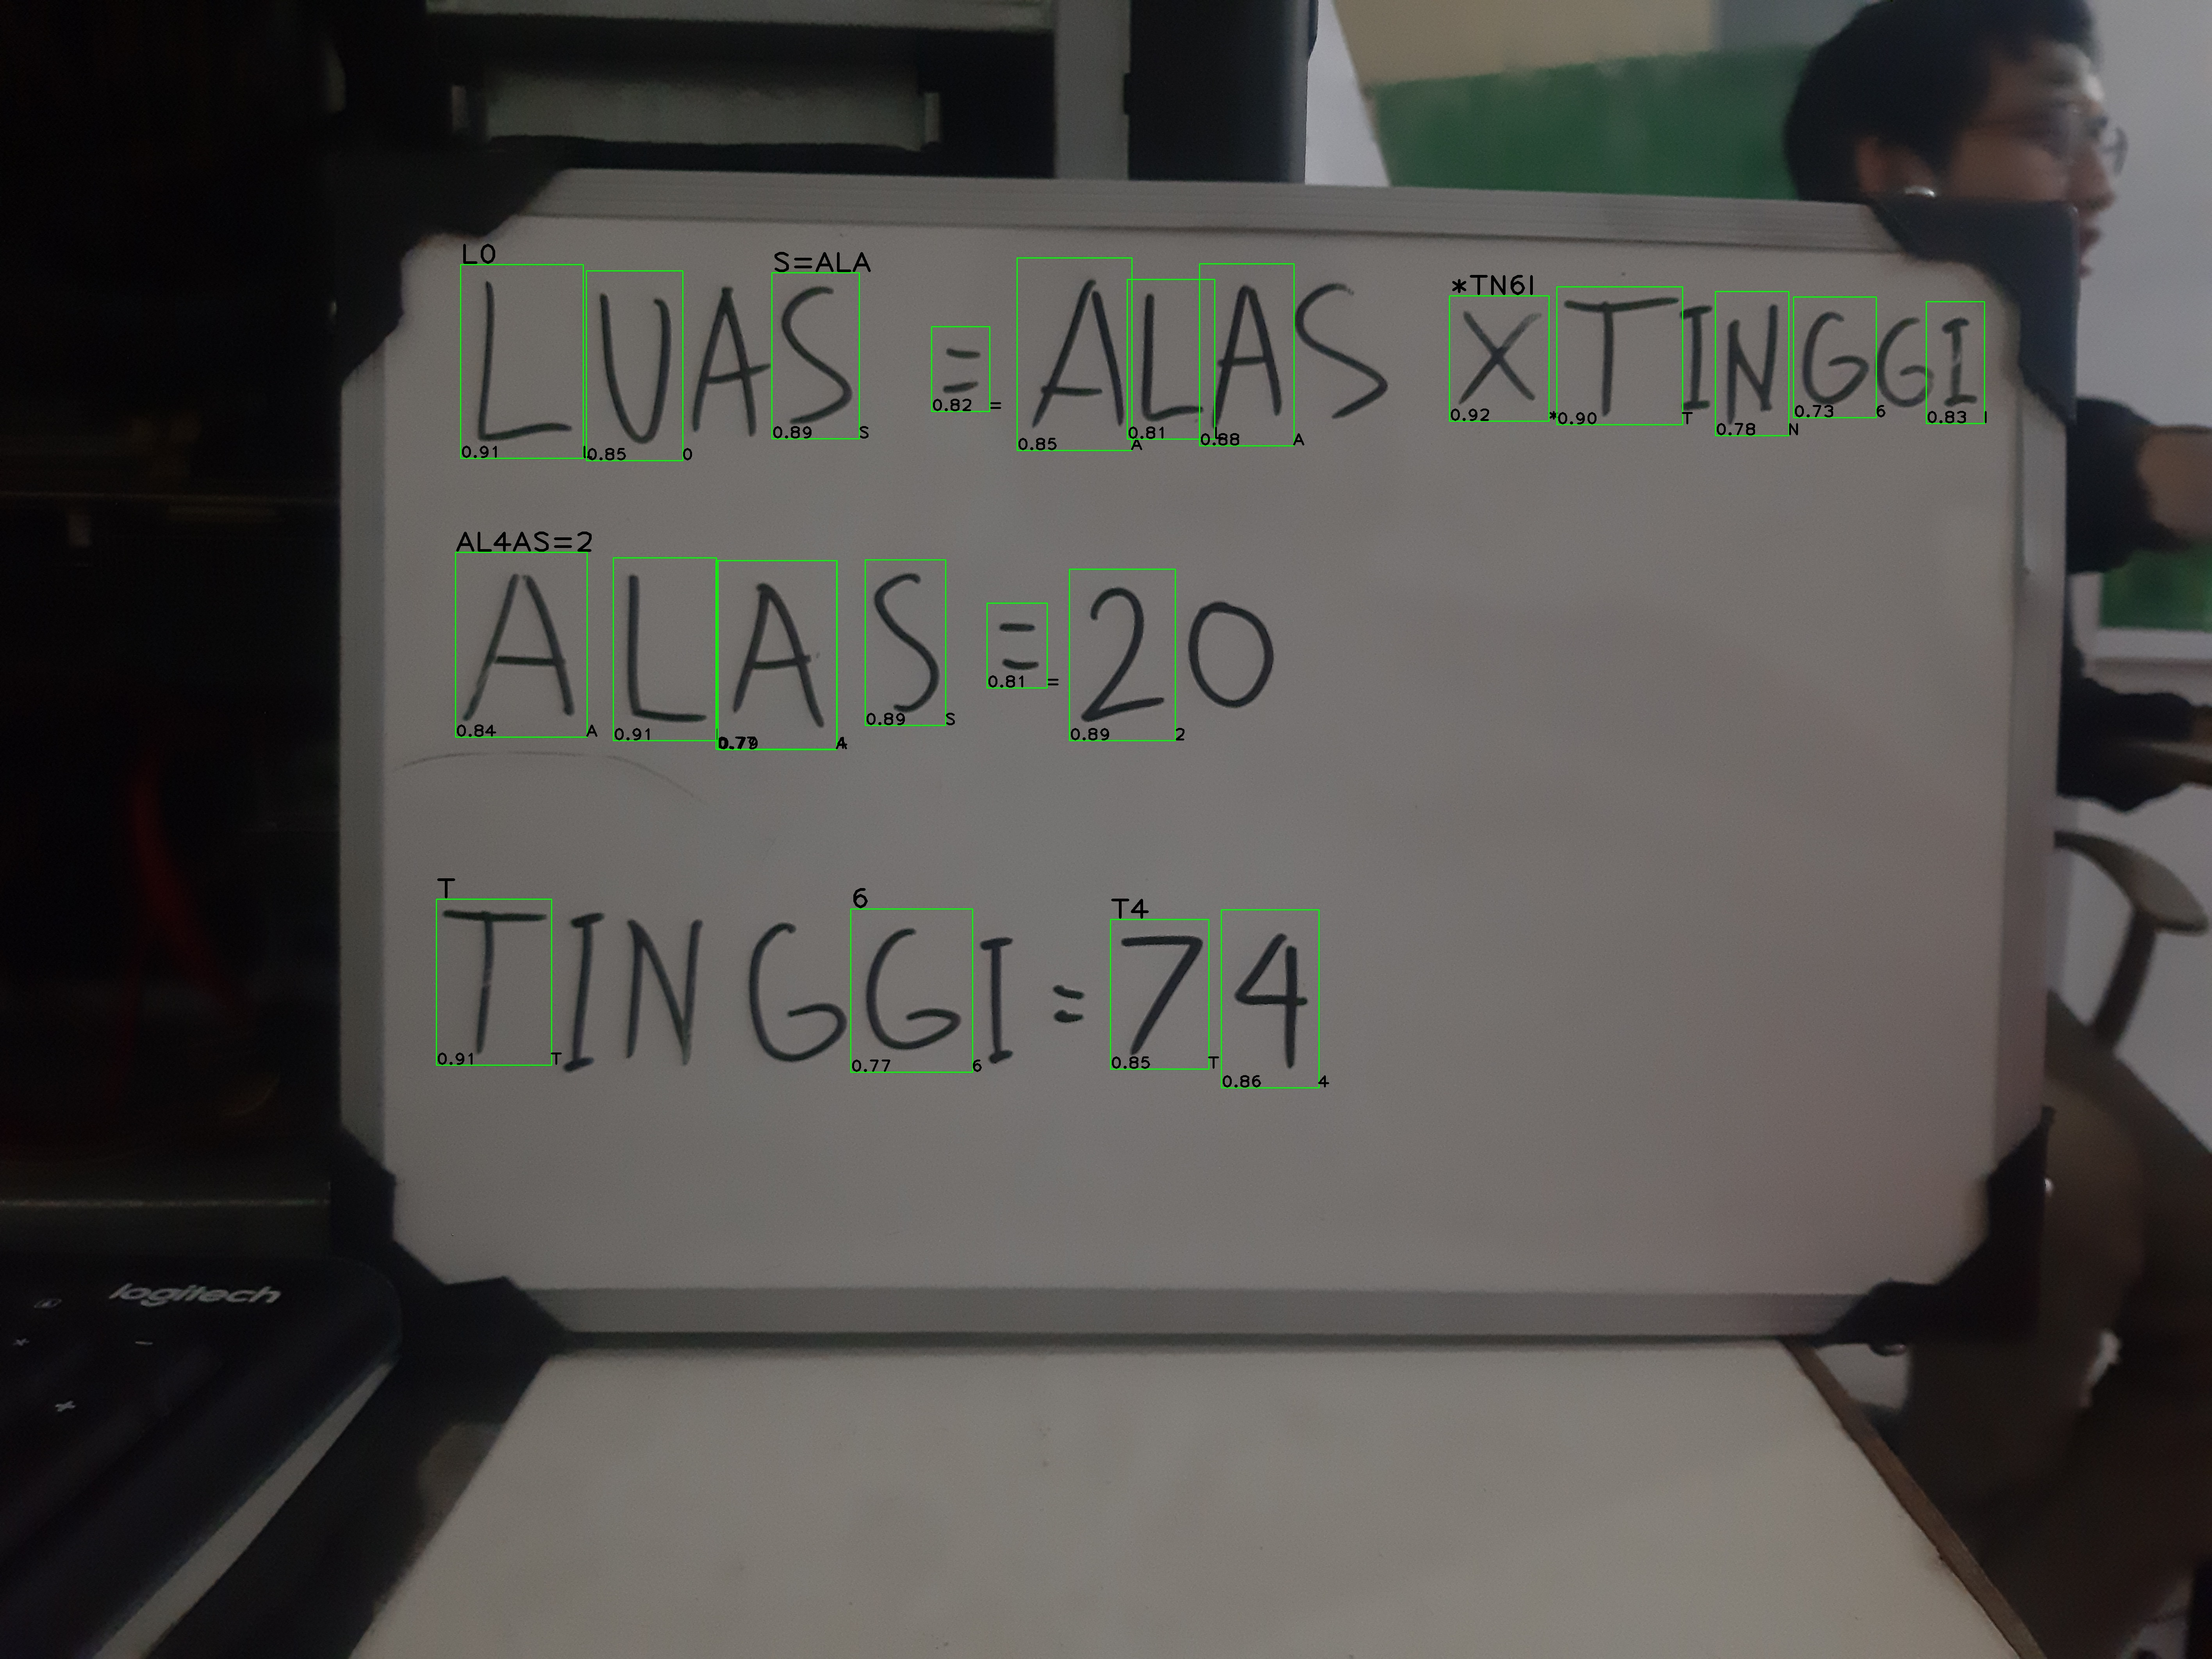
\includegraphics[width=.8\linewidth]{gambar/yolov5n/responden3/hans30cm10-result.jpg}
    \caption{Responden 3. Pengambilan Citra Jarak 30 Cm. Pencahayaan Gelap}
    \label{fig:nr3gcitra30cm}
  \end{subfigure}
  \caption{YOLOv5n. Responden 3. Pengambilan Citra Jarak 30 Cm}
  \label{fig:nr3citra30cm}
\end{figure}

% 40cm
\begin{figure}[H]
  \begin{subfigure}{.5\textwidth}
    \centering
    \captionsetup{width=.8\linewidth}
    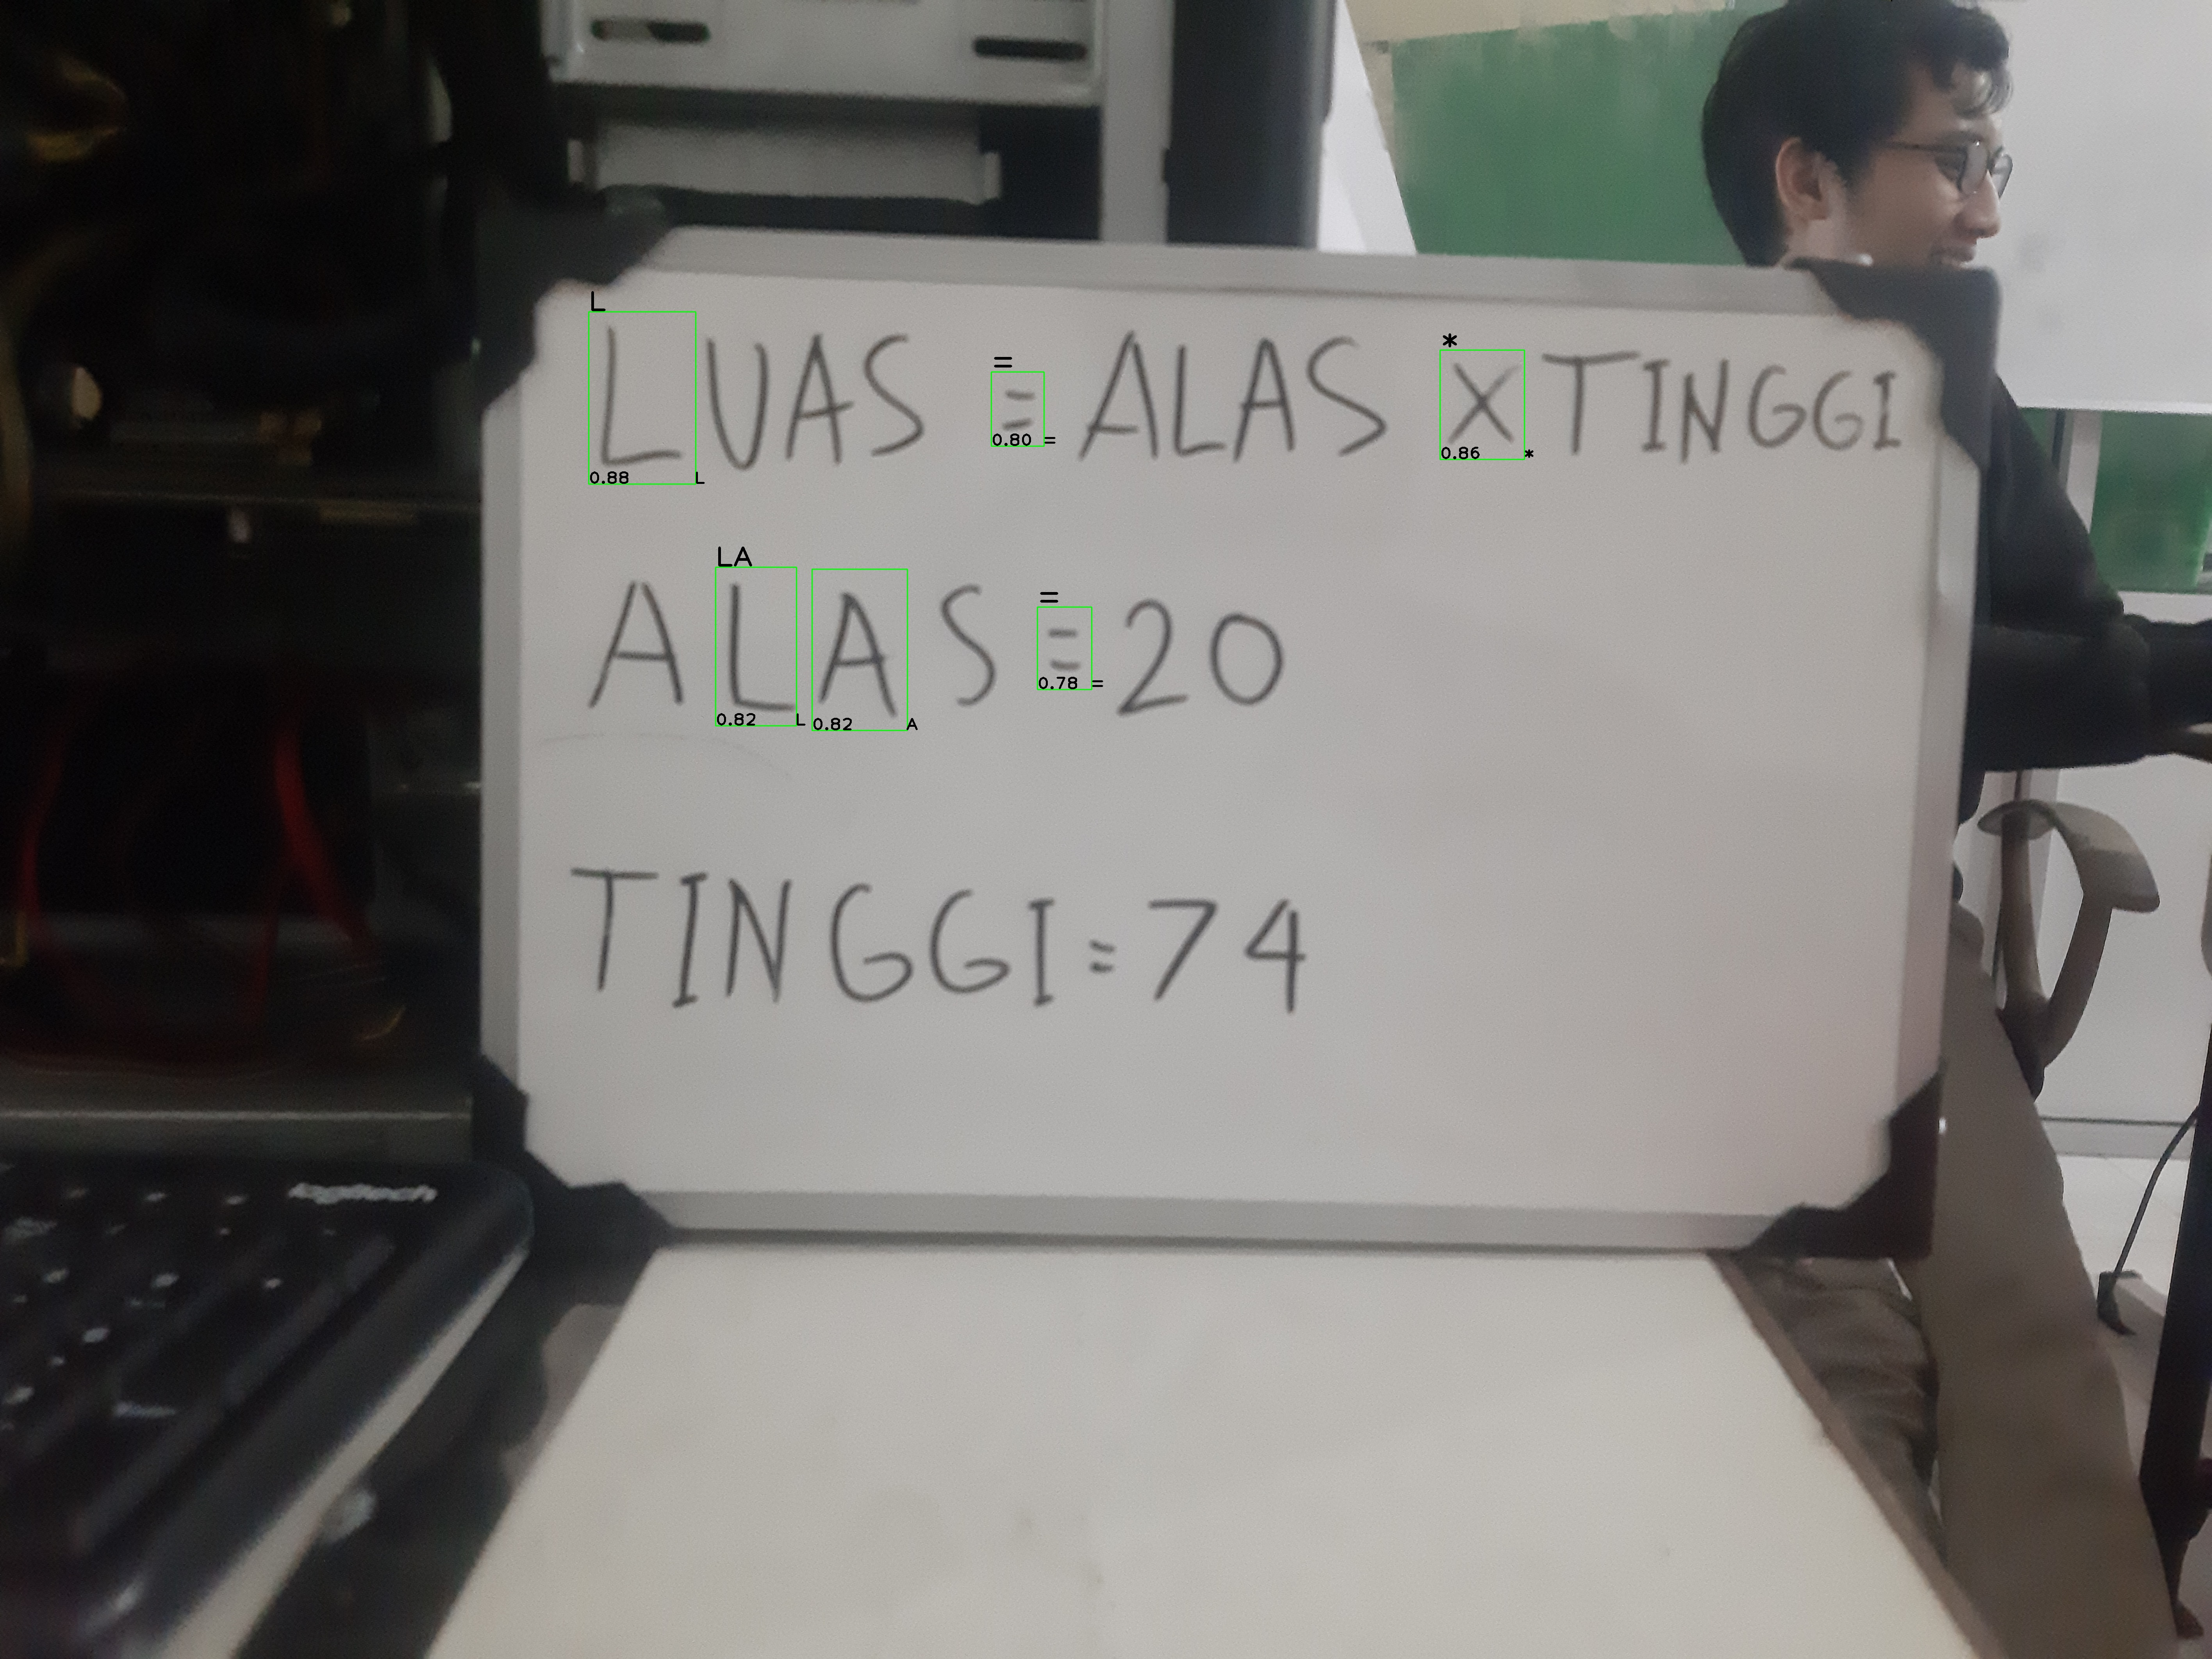
\includegraphics[width=.8\linewidth]{gambar/yolov5n/responden3/hans40cm00-result.jpg}
    \caption{Responden 3. Pengambilan Citra Jarak 40 Cm. Pencahayaan Normal}
    \label{fig:nr3tcitra40cm}
  \end{subfigure}%
  \begin{subfigure}{.5\textwidth}
    \centering
    \captionsetup{width=.8\linewidth}
    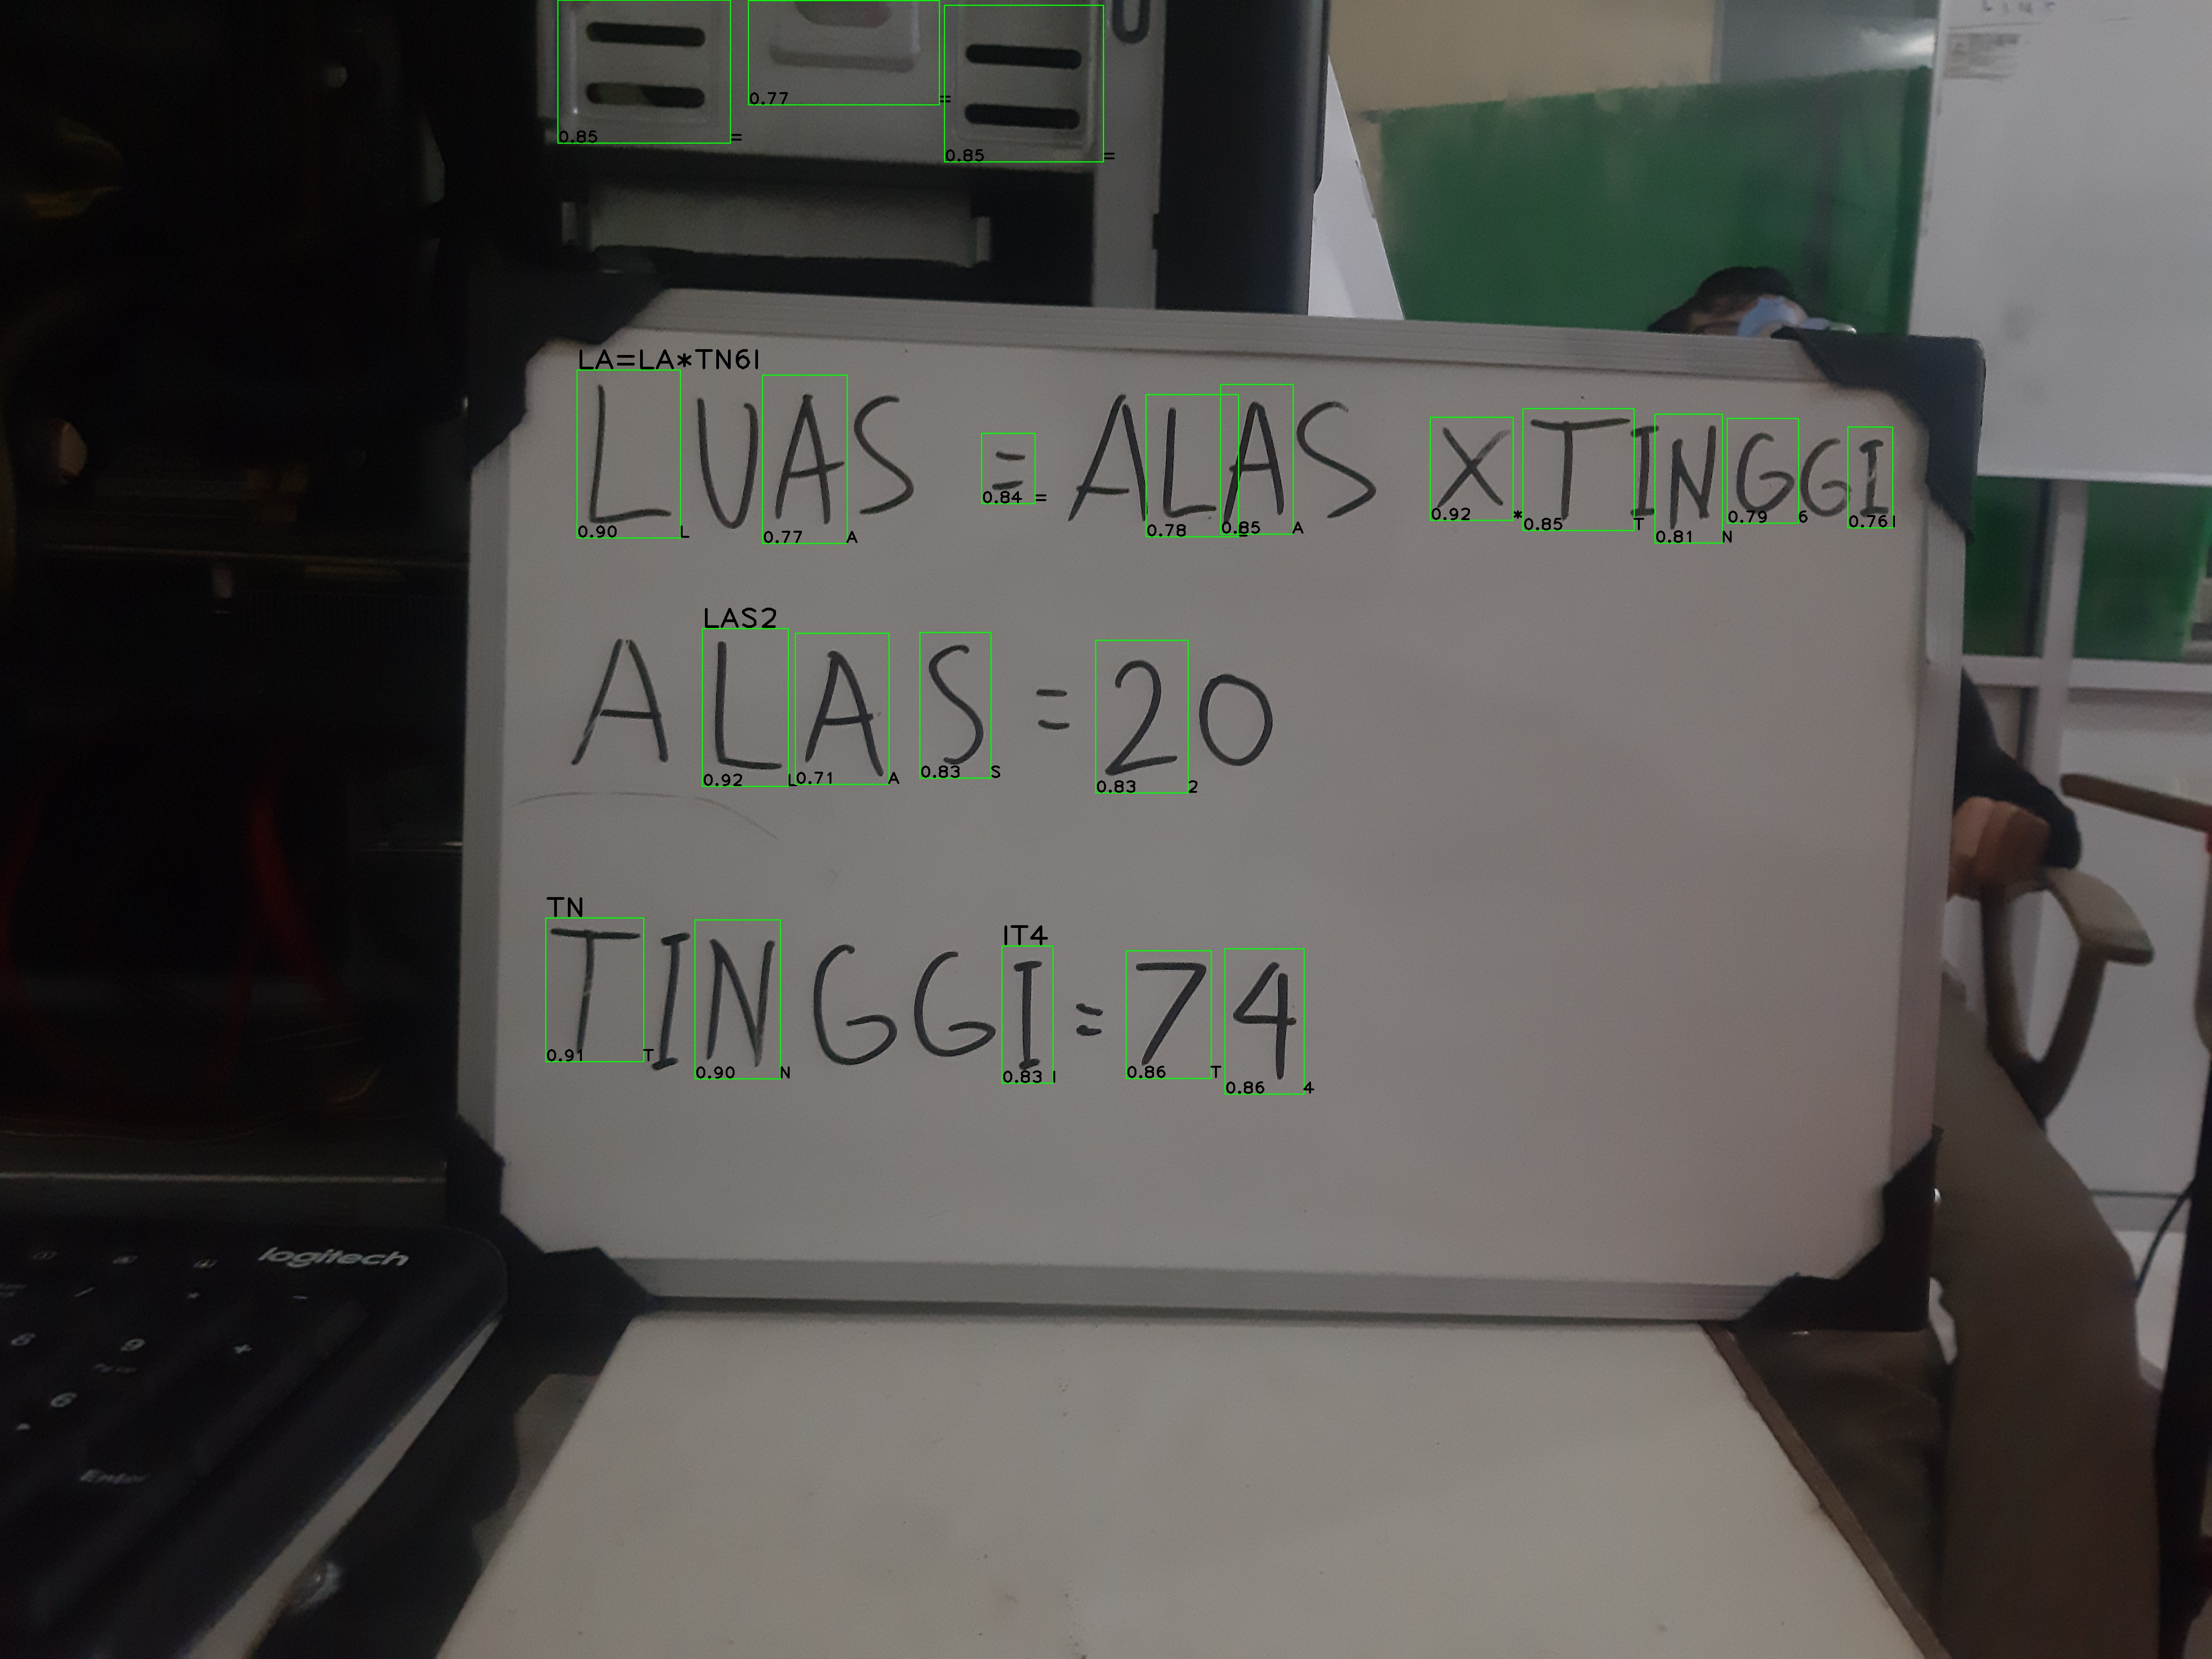
\includegraphics[width=.8\linewidth]{gambar/yolov5n/responden3/hans40cm10-result.jpg}
    \caption{Responden 3. Pengambilan Citra Jarak 40 Cm. Pencahayaan Gelap}
    \label{fig:nr3gcitra40cm}
  \end{subfigure}
  \caption{YOLOv5n. Responden 3. Pengambilan Citra Jarak 40 Cm}
  \label{fig:nr3citra40cm}
\end{figure}

Adapun secara umum, hasil pembacaan seluruh data dapat dilihat secara ringkas pada Tabel \ref*{tb:hasilresponden3yolov5n} berikut.

\begin{center}
  \begin{longtable}[c]{|l|c|c|c|c|}
    \caption{Hasil Pengujian pada Responden 3 menggunakan YOLOv5n}
    \label{tb:hasilresponden3yolov5n}\\
    \hline
    \multicolumn{1}{|c|}{\textbf{Citra}}                                       & \textbf{\begin{tabular}[c]{@{}c@{}}Total Objek\\ Pada Citra\end{tabular}} & \textbf{\begin{tabular}[c]{@{}c@{}}Objek Terbaca\\ Benar\end{tabular}} & \textbf{\begin{tabular}[c]{@{}c@{}}Objek Terbaca\\ Salah\end{tabular}} & \textbf{\begin{tabular}[c]{@{}c@{}}Objek Tidak\\ Terbaca\end{tabular}} \\ \hline
    \endhead
    %
    \begin{tabular}[c]{@{}l@{}}Jarak 20cm\\ Pencahayaan \\ Terang\end{tabular} & 32    & 20     & 0     & 12       \\ \hline
    \begin{tabular}[c]{@{}l@{}}Jarak 20cm\\ Pencahayaan \\ Gelap\end{tabular}  & 32    & 15     & 1     & 16       \\ \hline
    \begin{tabular}[c]{@{}l@{}}Jarak 30cm\\ Pencahayaan \\ Terang\end{tabular} & 32    & 8     & 1     & 23       \\ \hline
    \begin{tabular}[c]{@{}l@{}}Jarak 30cm\\ Pencahayaan \\ Gelap\end{tabular}  & 32    & 11     & 1     & 20       \\ \hline
    \begin{tabular}[c]{@{}l@{}}Jarak 40cm\\ Pencahayaan \\ Terang\end{tabular} & 32    & 6     & 0     & 26       \\ \hline
    \begin{tabular}[c]{@{}l@{}}Jarak 40cm\\ Pencahayaan \\ Gelap\end{tabular}  & 32    & 8     & 2     & 24       \\ \hline
  \end{longtable}
\end{center}

\subsubsection{Skenario Pengujian Menggunakan Data Citra dari Responden 4}
\label{subsubsec:nskenarioresponden4}

Pada pengujian pembacaan citra dari responden 4, data yang akan diuji dibagi menjadi skenario berdasarkan jarak pengambilan citra dan tingkat pencahayaan citra. Adapun hasil pembacaan yaitu didapatkan hasil yaitu seperti pada Gambar \ref*{fig:nr4citra20cm}, Gambar \ref*{fig:nr4citra30cm}, dan Gambar \ref*{fig:nr4citra40cm}.

% 20cm
\begin{figure}[H]
  \begin{subfigure}{.5\textwidth}
    \centering
    \captionsetup{width=.8\linewidth}
    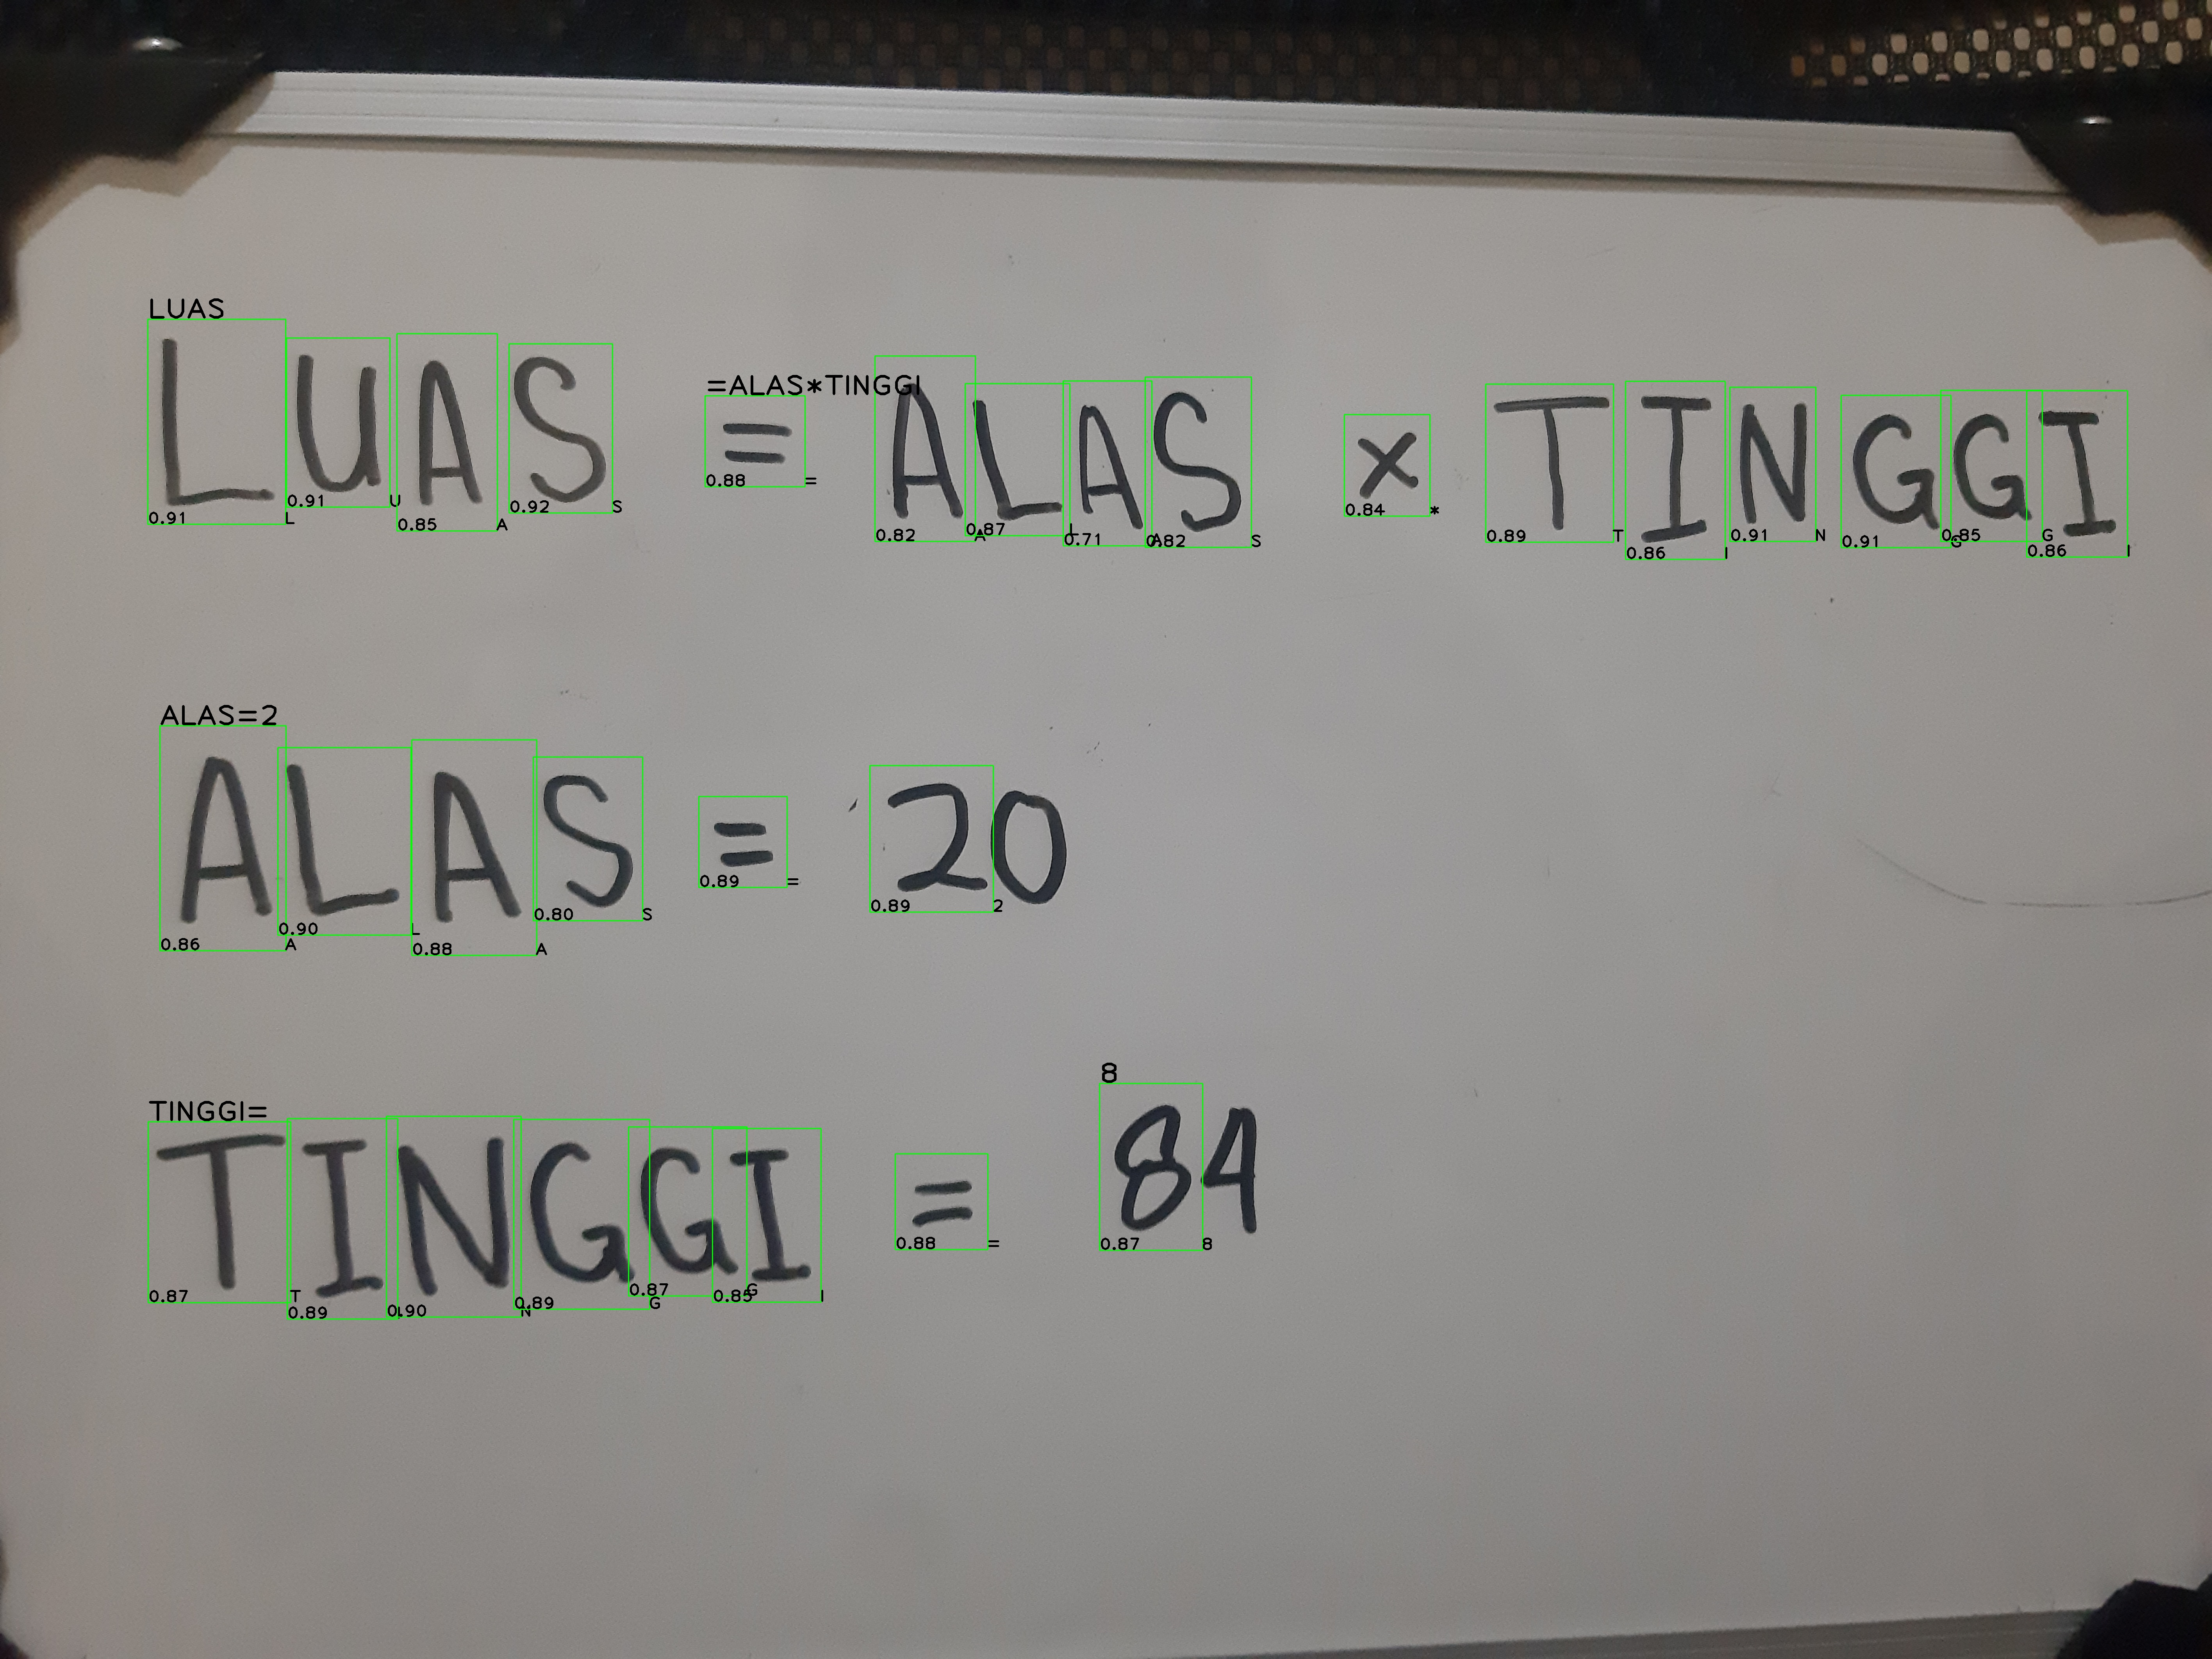
\includegraphics[width=.8\linewidth]{gambar/yolov5n/responden4/hakimaxt20cm00-result.jpg}
    \caption{Responden 4. Pengambilan Citra Jarak 20 Cm. Pencahayaan Normal}
    \label{fig:nr4tcitra20cm}
  \end{subfigure}%
  \begin{subfigure}{.5\textwidth}
    \centering
    \captionsetup{width=.8\linewidth}
    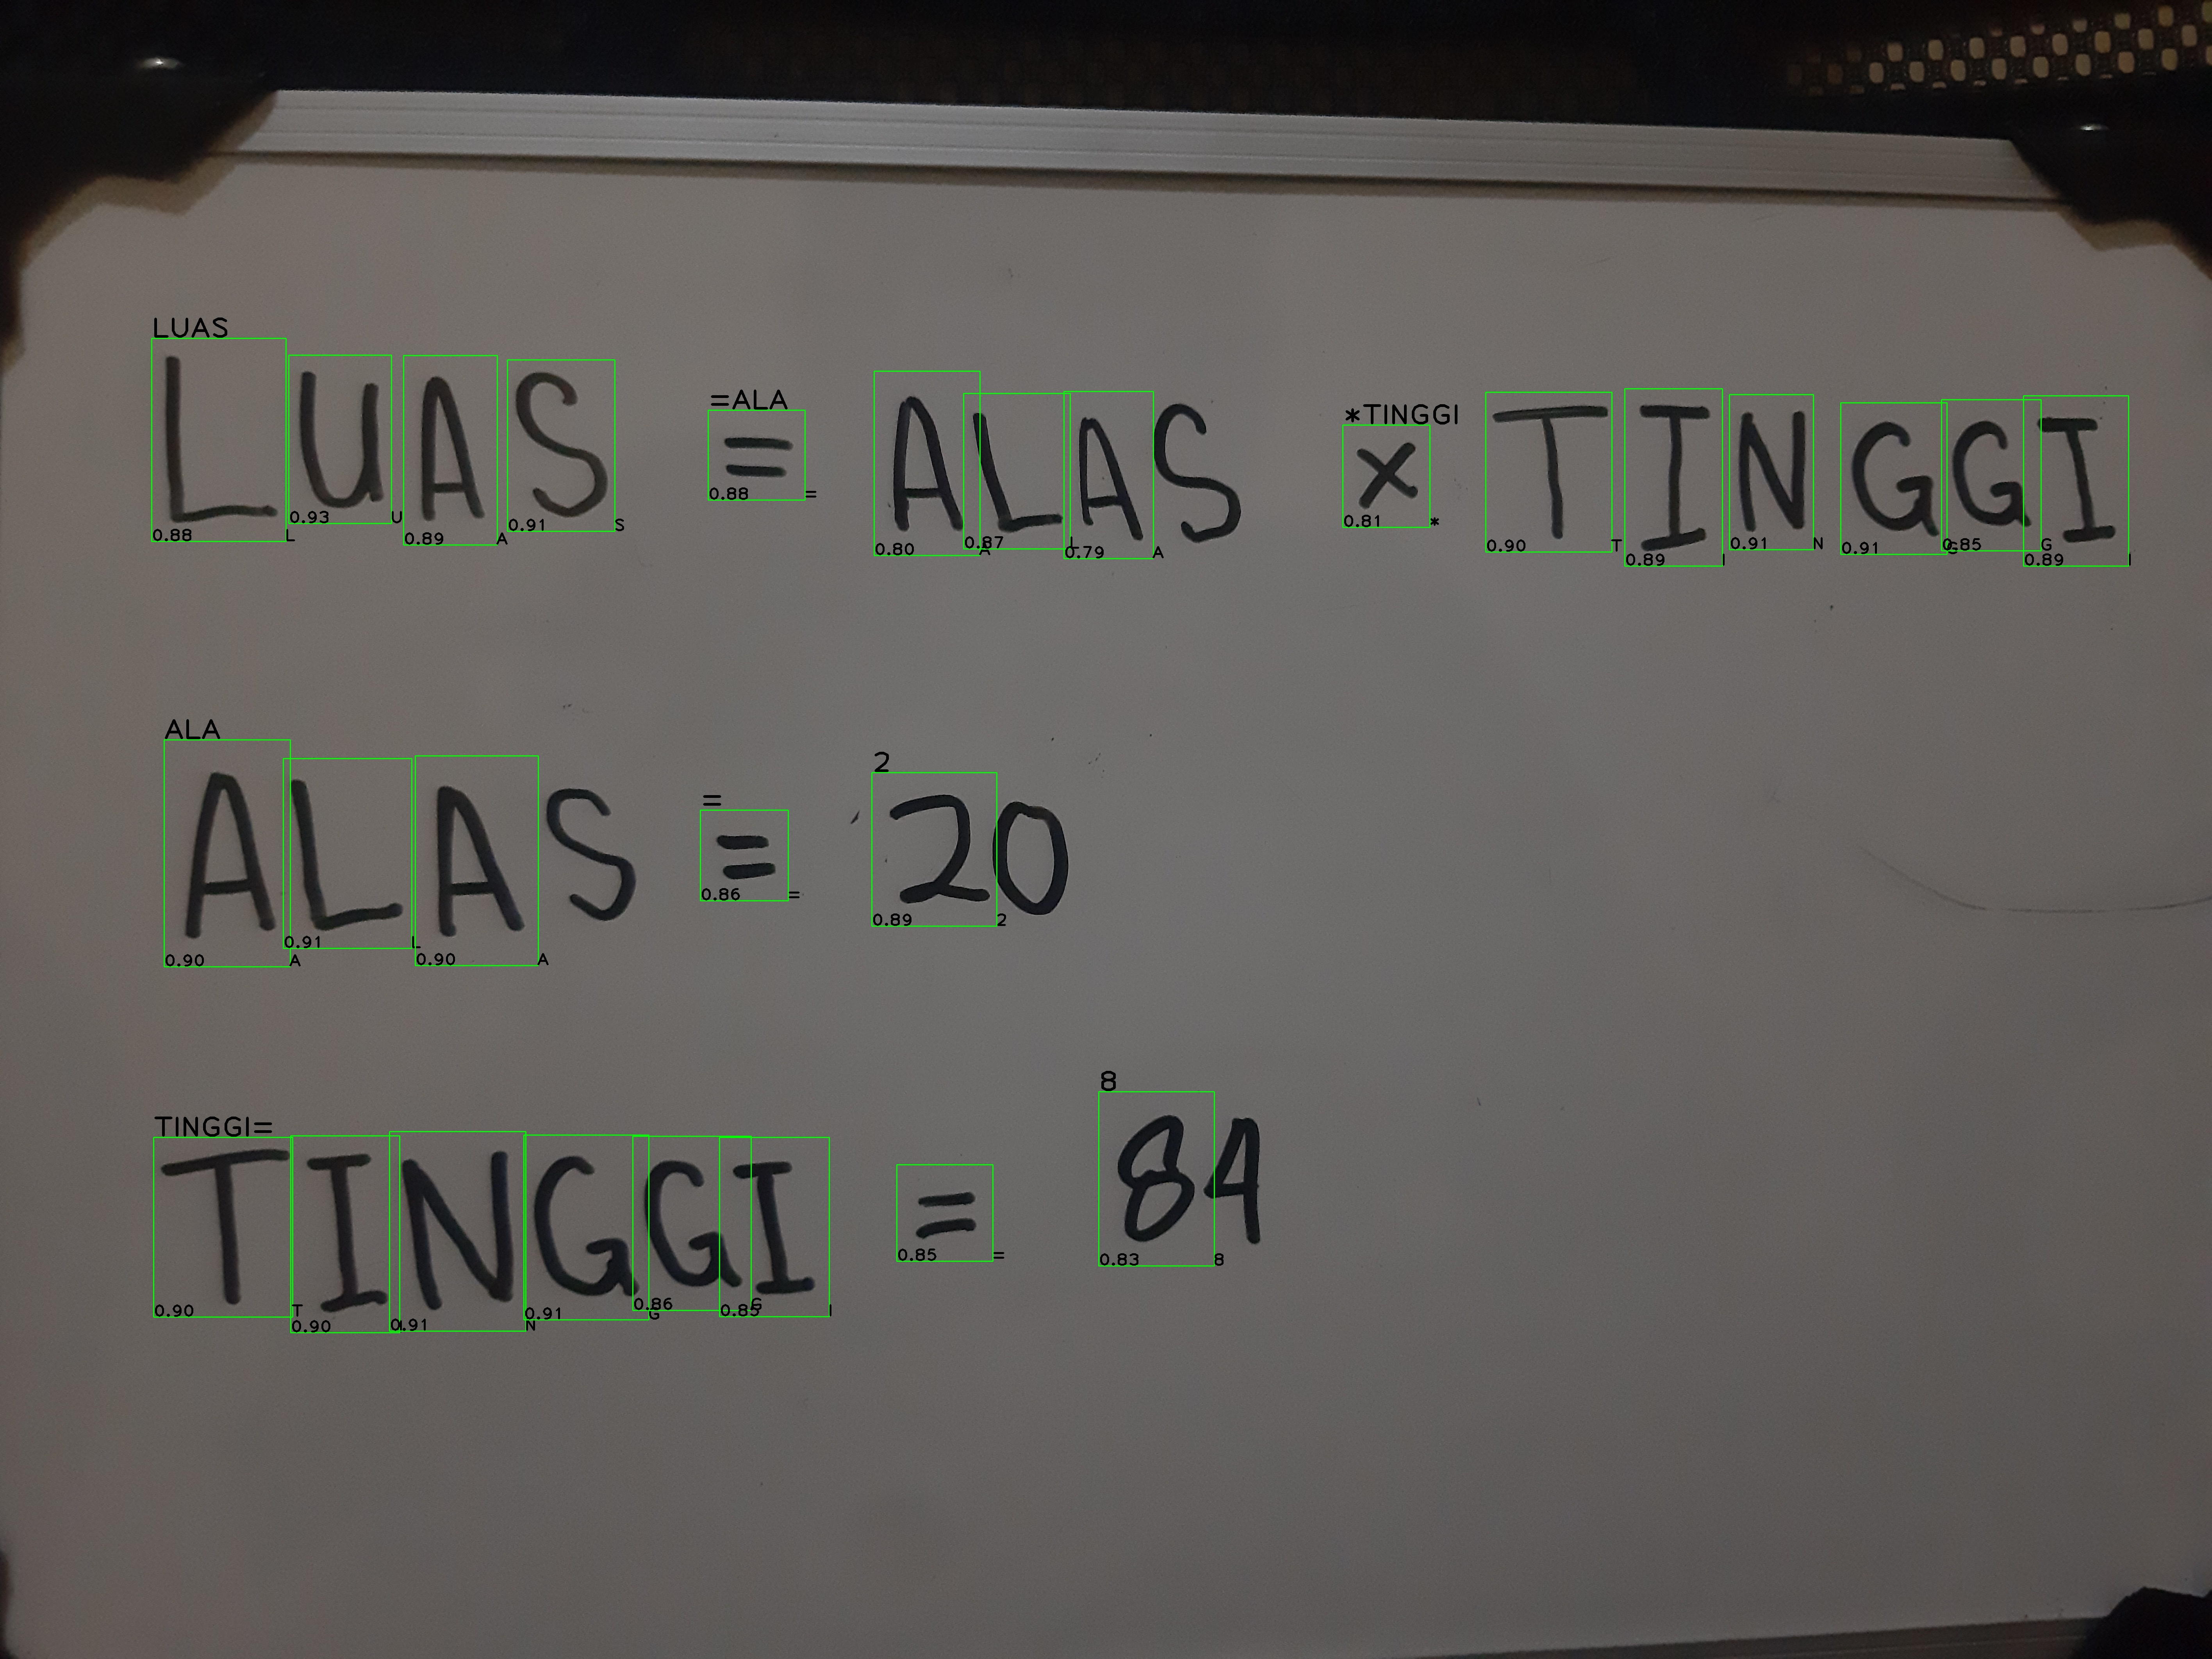
\includegraphics[width=.8\linewidth]{gambar/yolov5n/responden4/hakimaxt20cm10-result.jpg}
    \caption{Responden 4. Pengambilan Citra Jarak 20 Cm. Pencahayaan Gelap}
    \label{fig:nr4gcitra20cm}
  \end{subfigure}
  \caption{YOLOv5n. Responden 4. Pengambilan Citra Jarak 20 Cm}
  \label{fig:nr4citra20cm}
\end{figure}

% 30cm
\begin{figure}[H]
  \begin{subfigure}{.5\textwidth}
    \centering
    \captionsetup{width=.8\linewidth}
    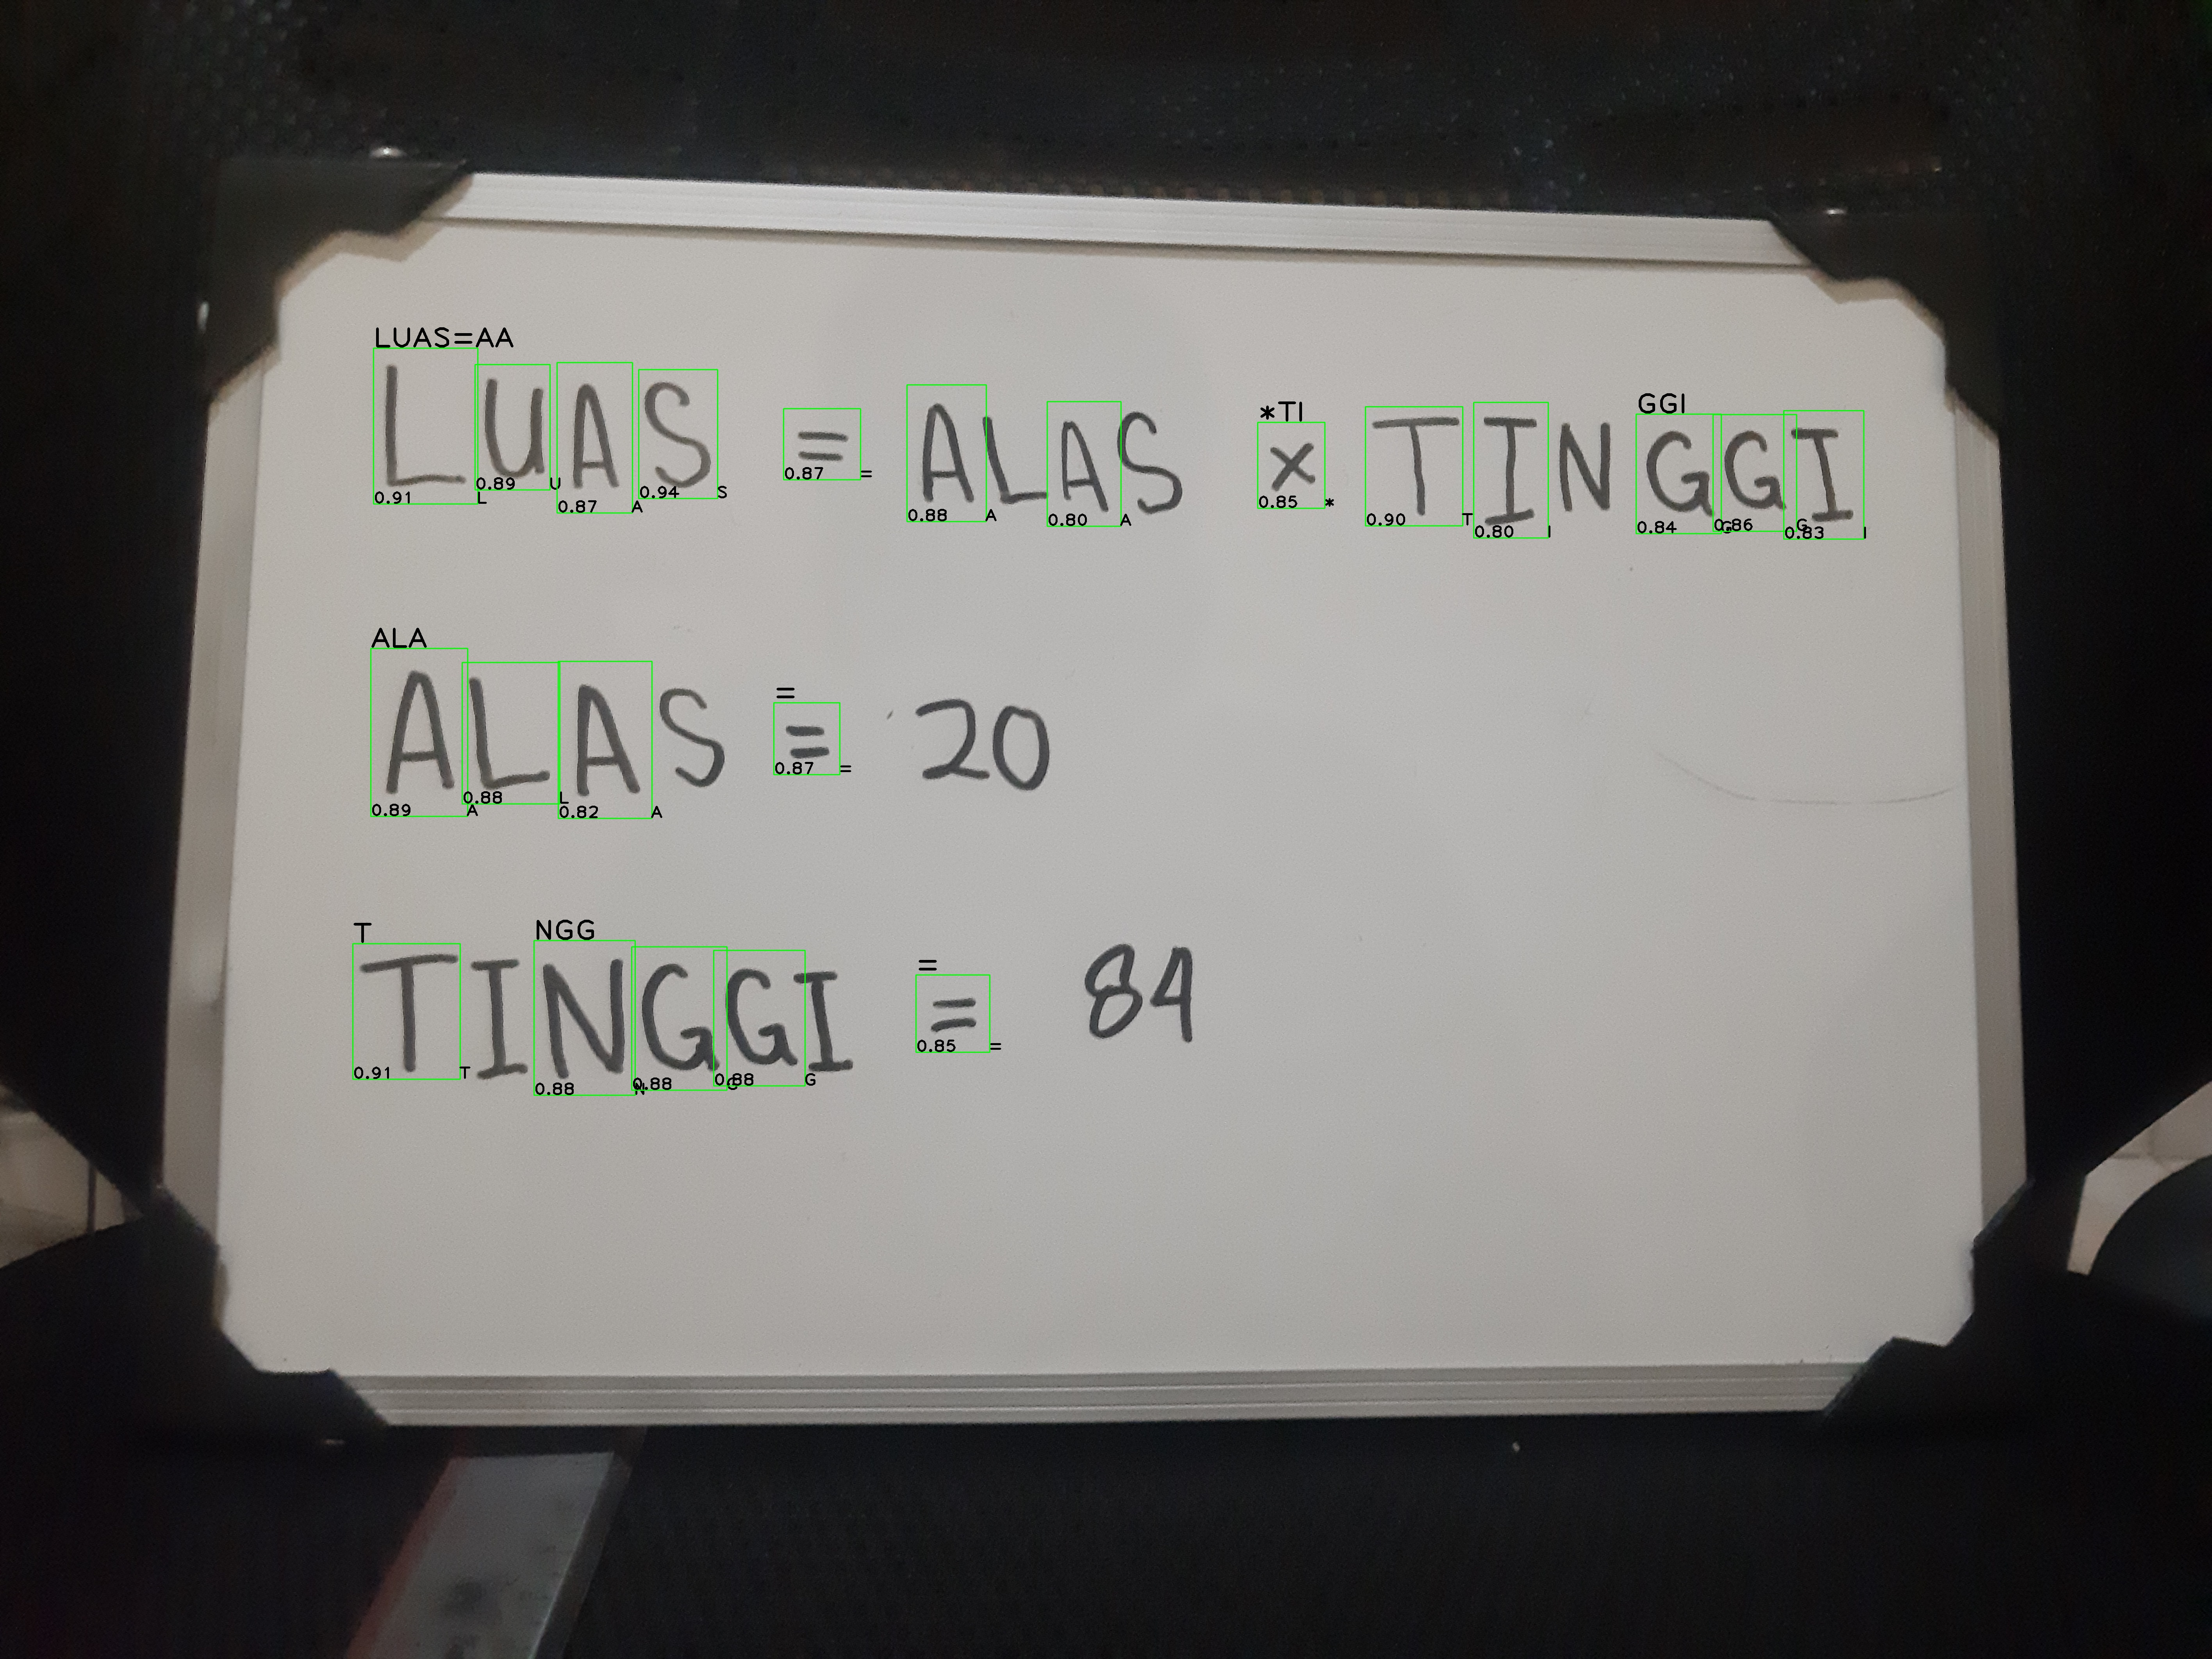
\includegraphics[width=.8\linewidth]{gambar/yolov5n/responden4/hakimaxt30cm00-result.jpg}
    \caption{Responden 4. Pengambilan Citra Jarak 30 Cm. Pencahayaan Normal}
    \label{fig:nr4tcitra30cm}
  \end{subfigure}%
  \begin{subfigure}{.5\textwidth}
    \centering
    \captionsetup{width=.8\linewidth}
    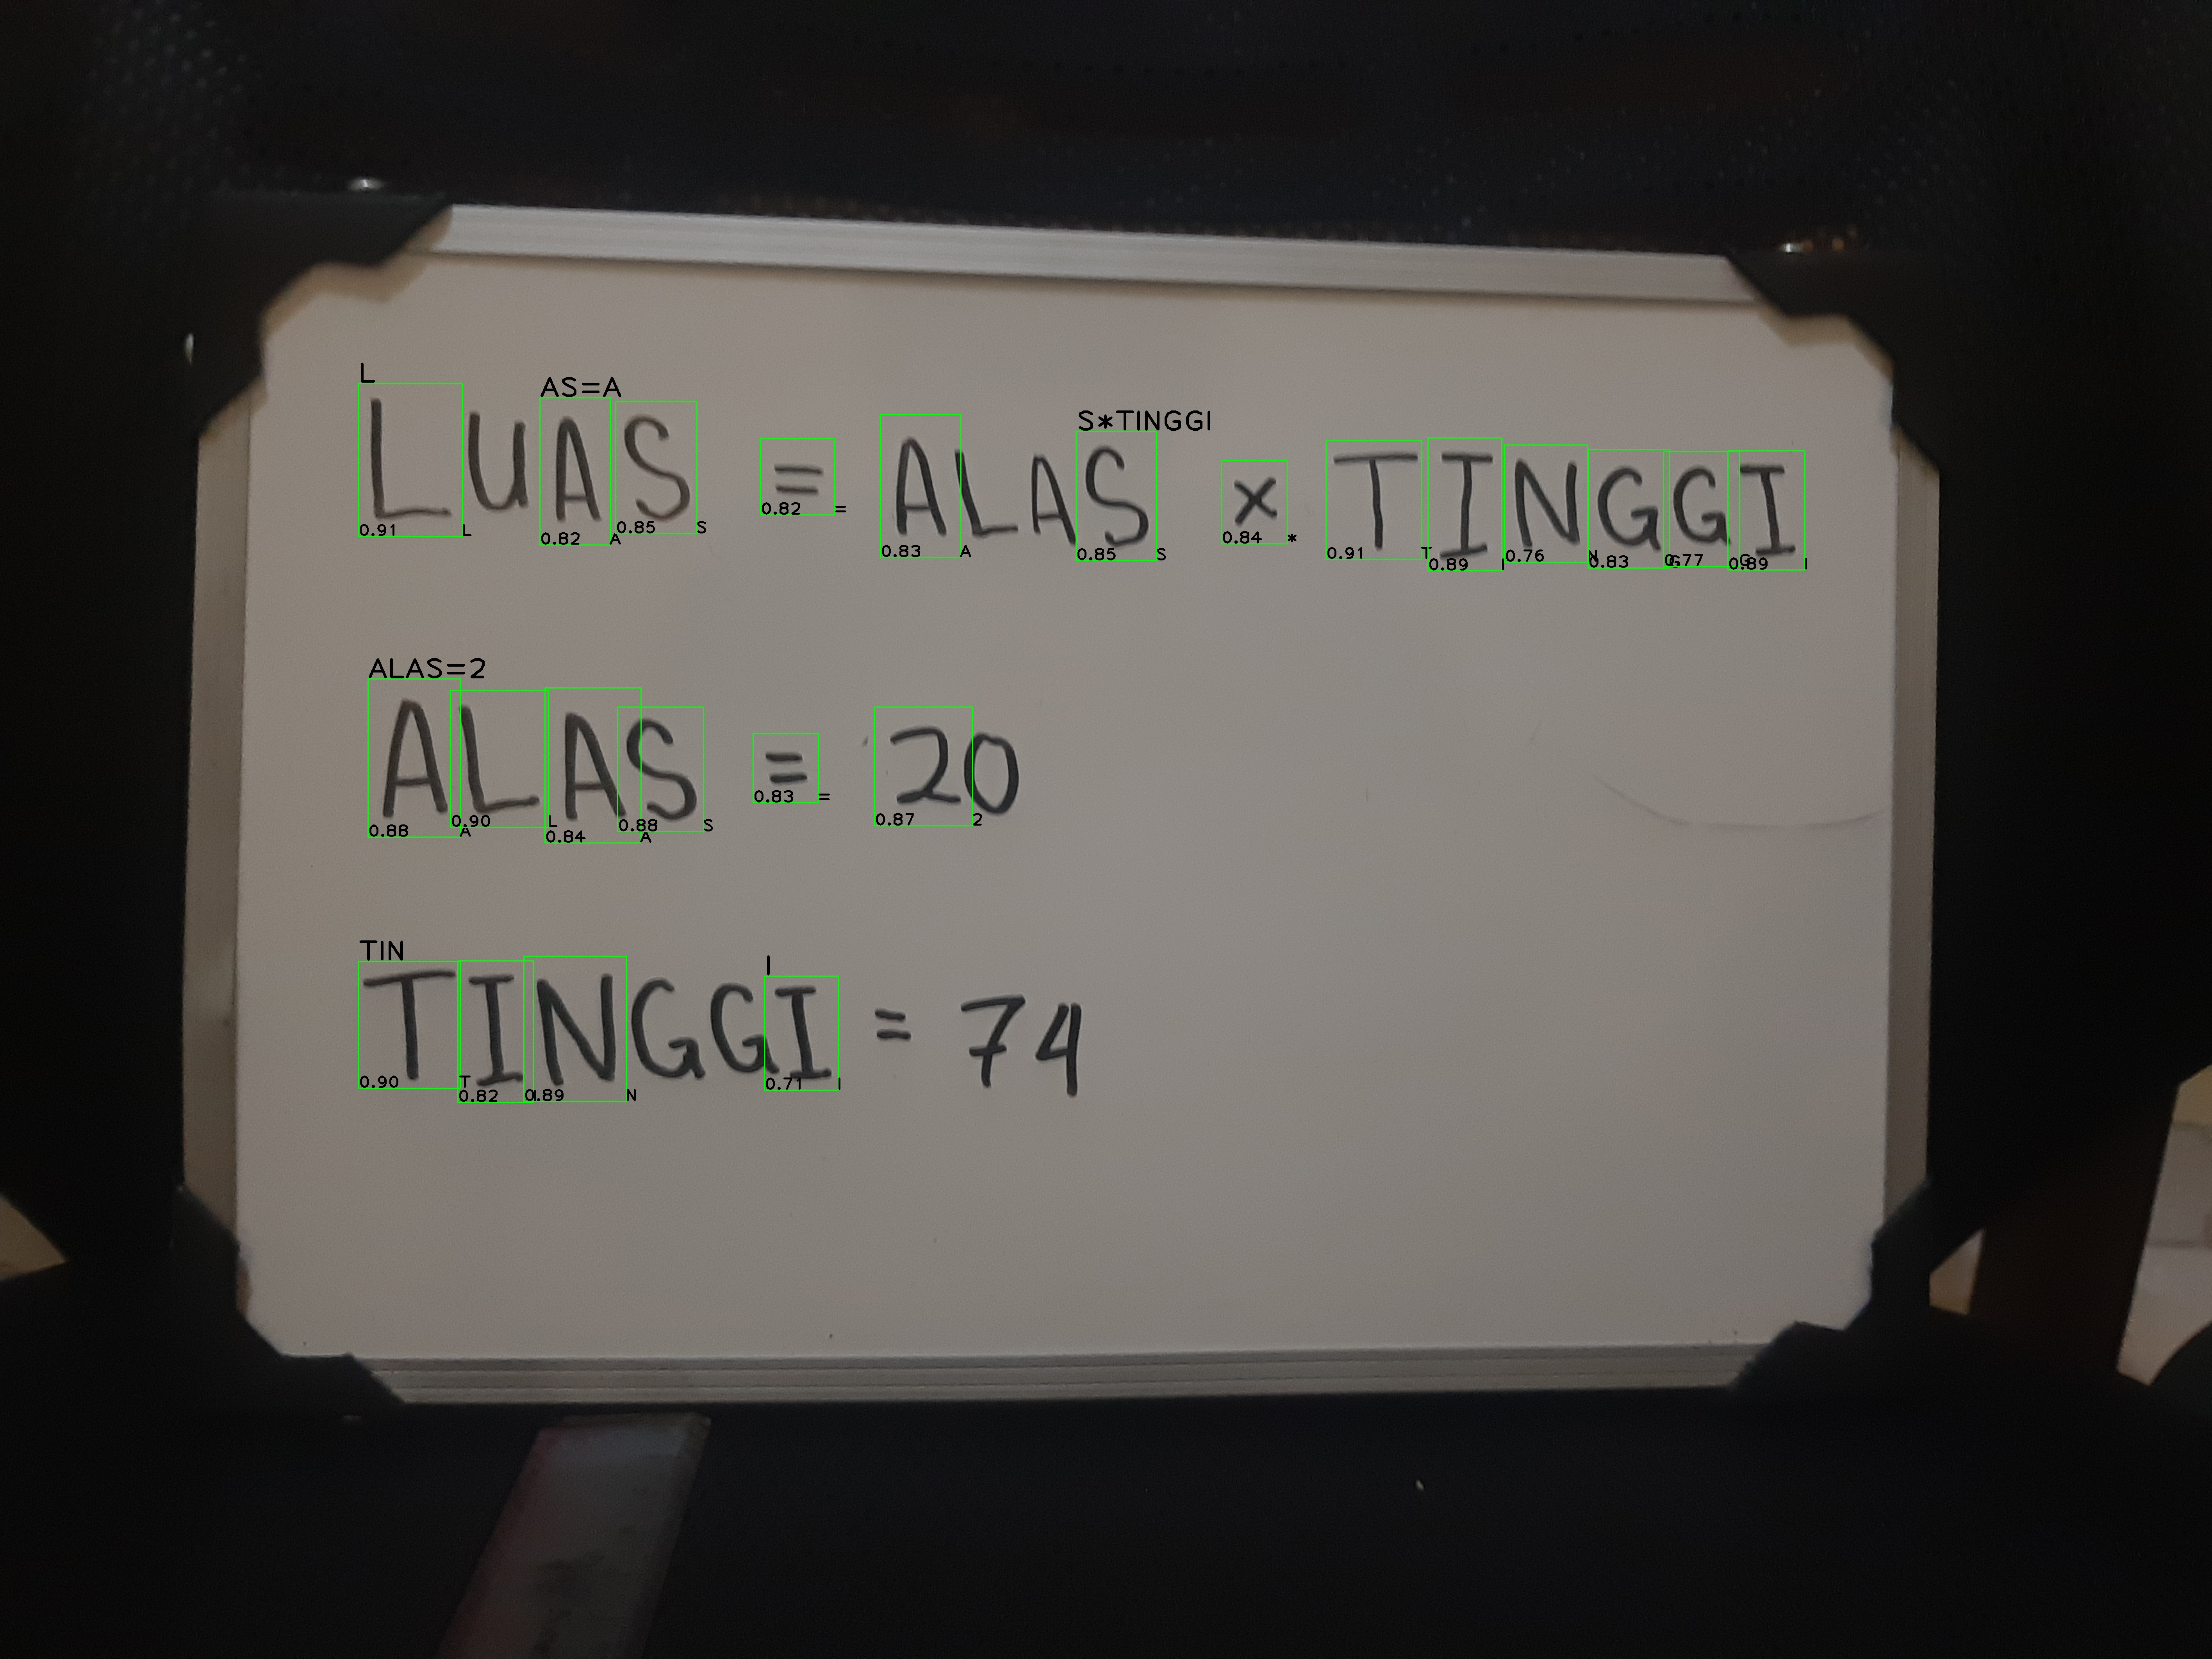
\includegraphics[width=.8\linewidth]{gambar/yolov5n/responden4/hakimaxt30cm10-result.jpg}
    \caption{Responden 4. Pengambilan Citra Jarak 30 Cm. Pencahayaan Gelap}
    \label{fig:nr4gcitra30cm}
  \end{subfigure}
  \caption{YOLOv5n. Responden 4. Pengambilan Citra Jarak 30 Cm}
  \label{fig:nr4citra30cm}
\end{figure}

% 40cm
\begin{figure}[H]
  \begin{subfigure}{.5\textwidth}
    \centering
    \captionsetup{width=.8\linewidth}
    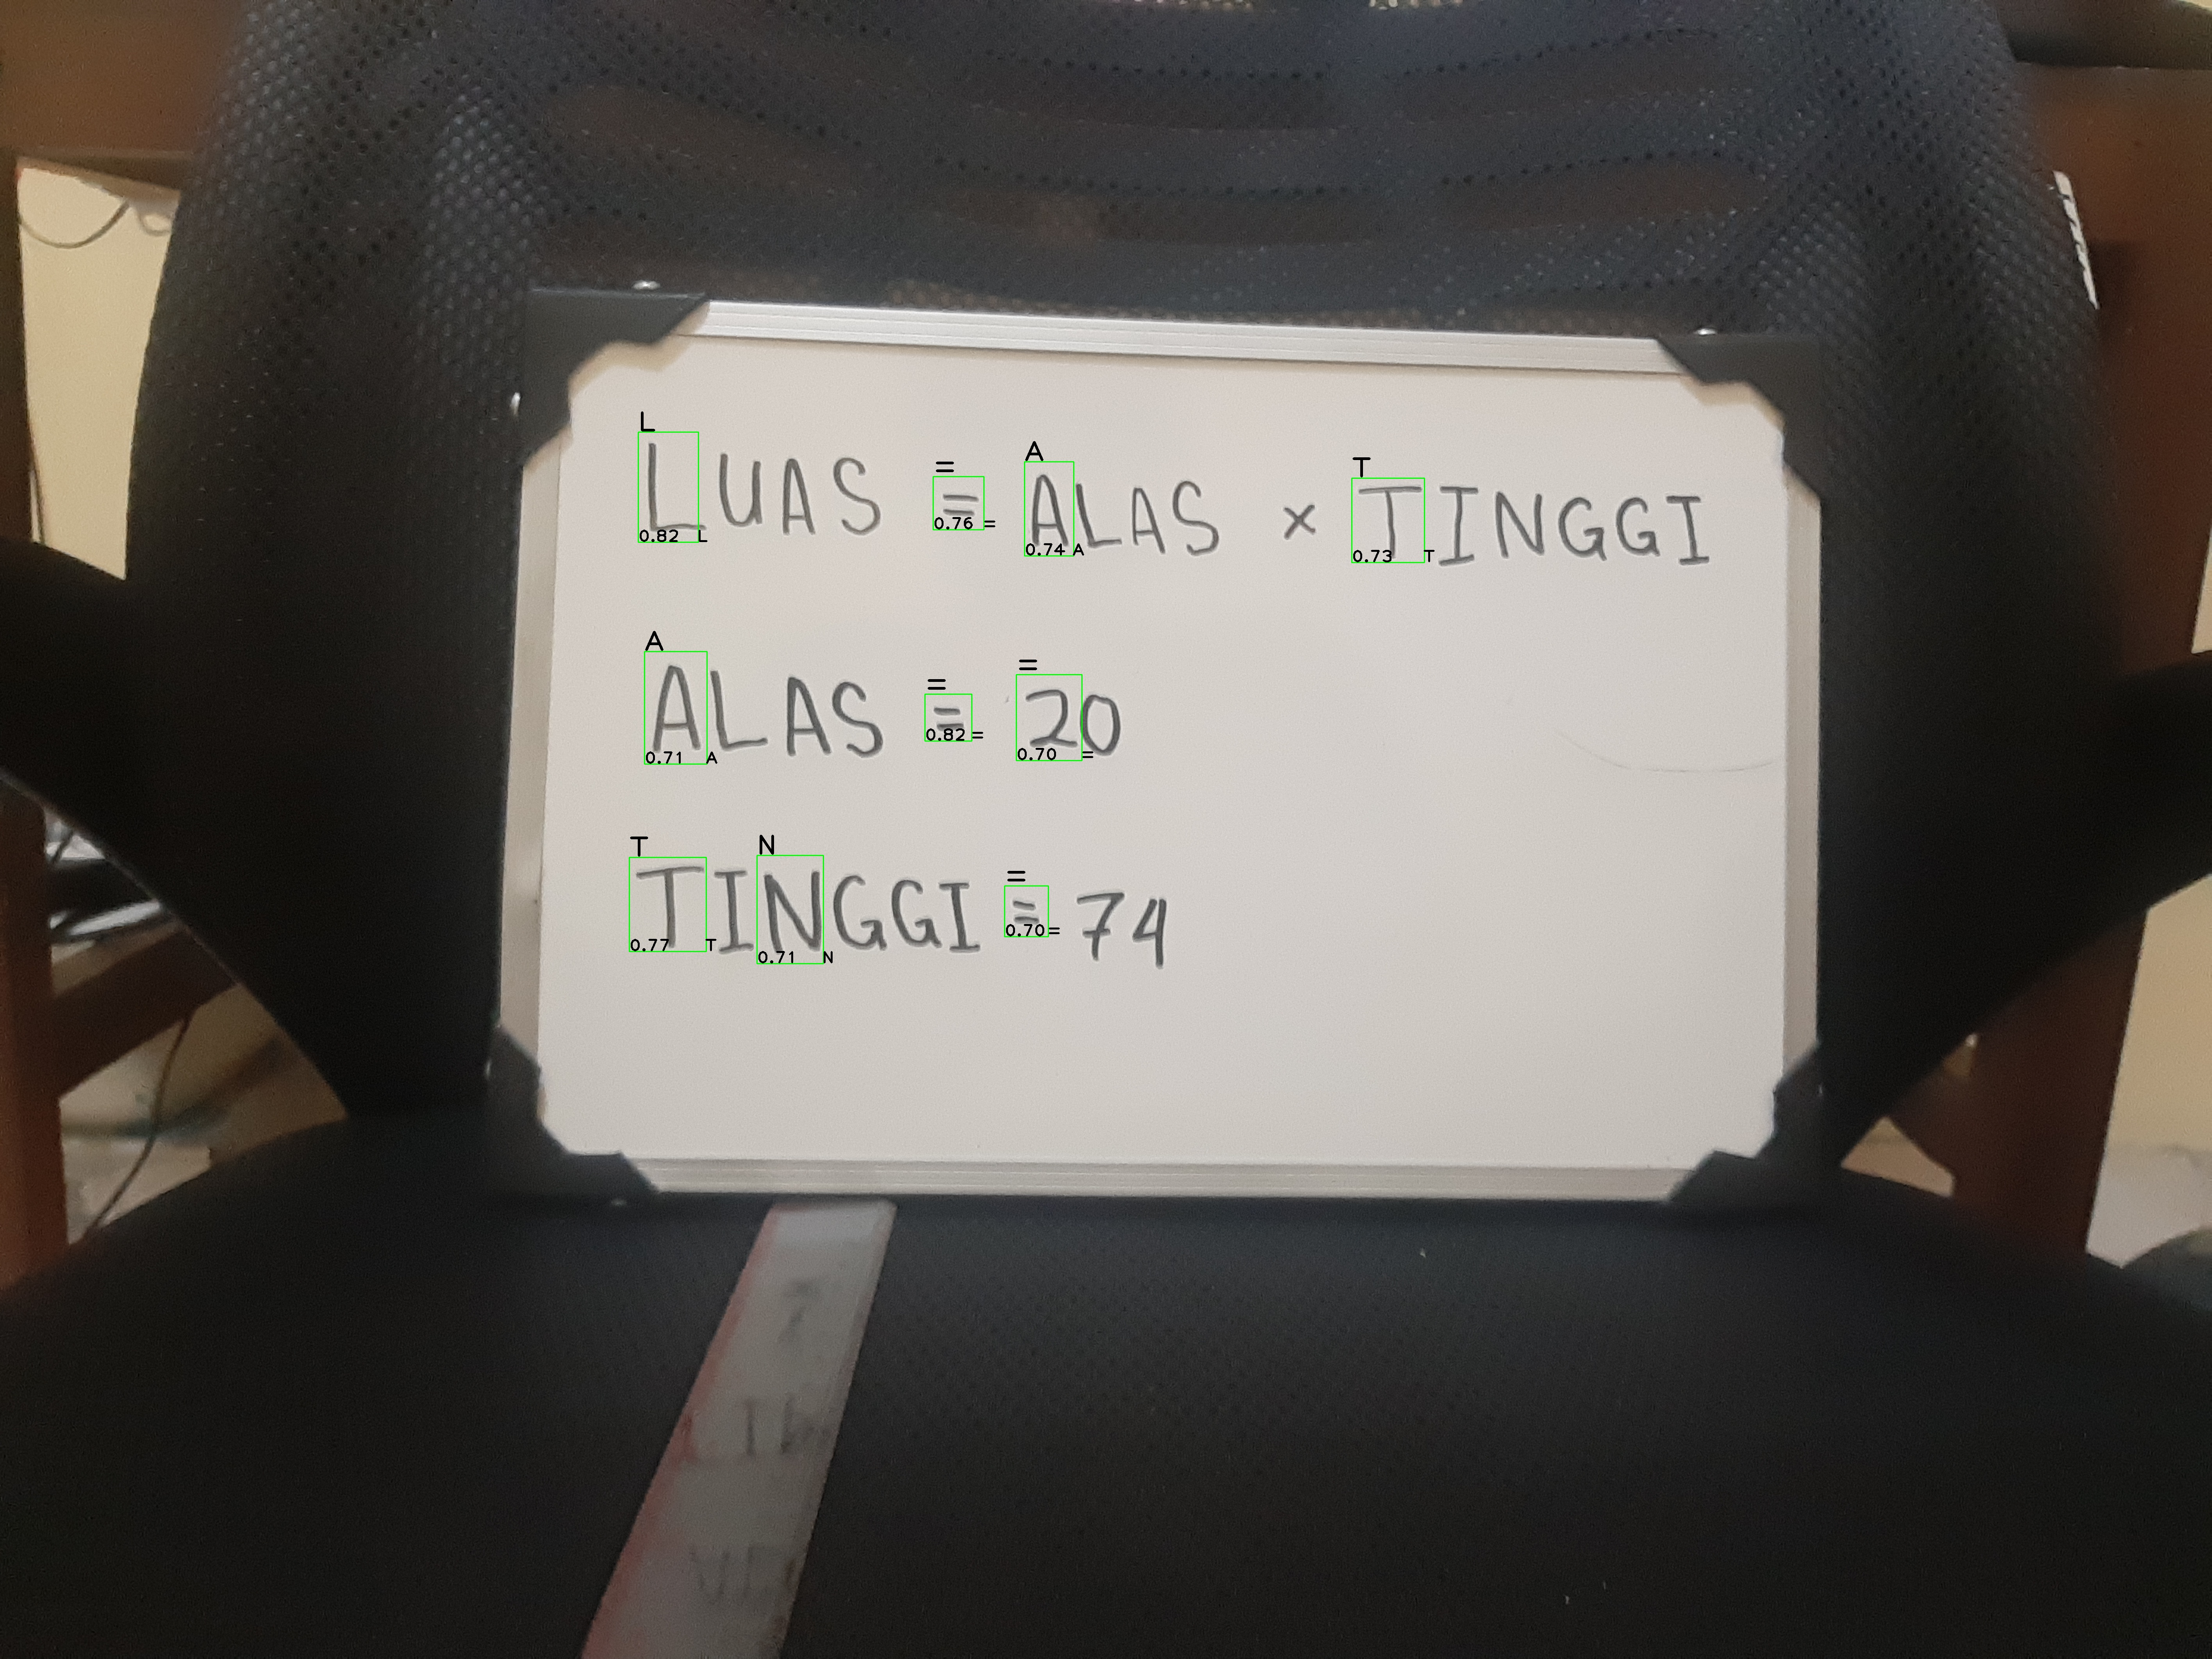
\includegraphics[width=.8\linewidth]{gambar/yolov5n/responden4/hakimaxt40cm00-result.jpg}
    \caption{Responden 4. Pengambilan Citra Jarak 40 Cm. Pencahayaan Normal}
    \label{fig:nr4tcitra40cm}
  \end{subfigure}%
  \begin{subfigure}{.5\textwidth}
    \centering
    \captionsetup{width=.8\linewidth}
    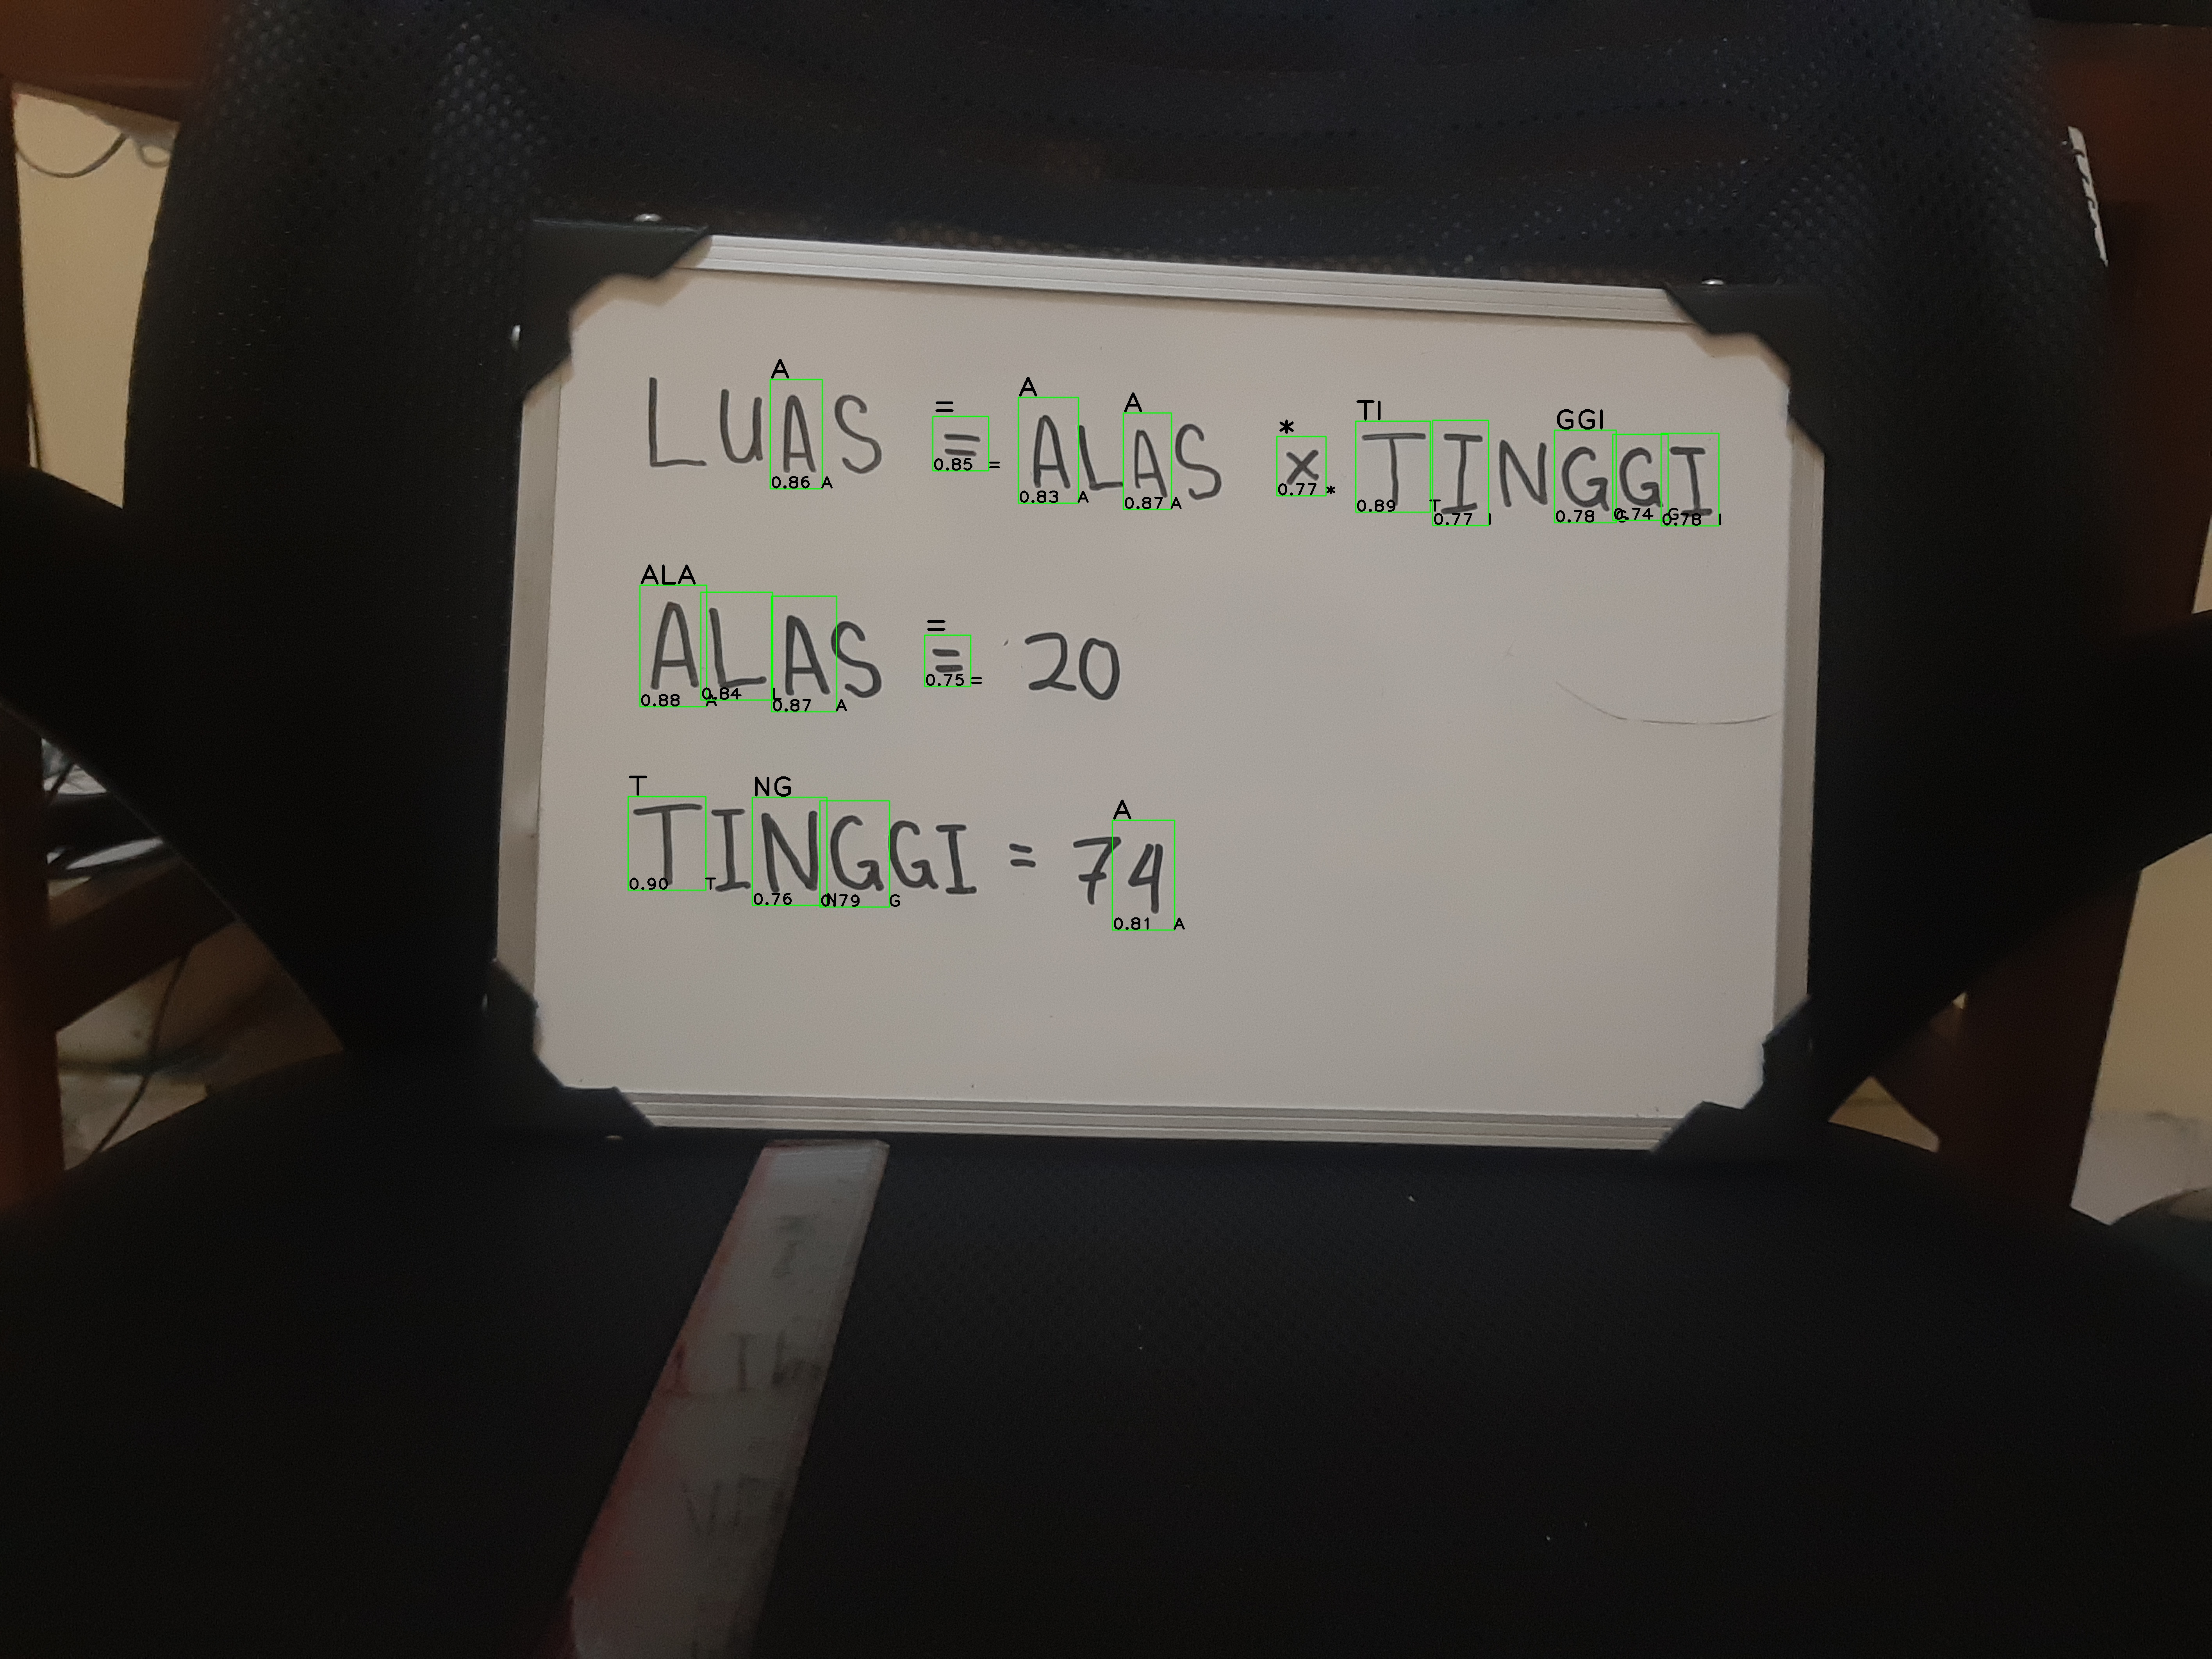
\includegraphics[width=.8\linewidth]{gambar/yolov5n/responden4/hakimaxt40cm10-result.jpg}
    \caption{Responden 4. Pengambilan Citra Jarak 40 Cm. Pencahayaan Gelap}
    \label{fig:nr4gcitra40cm}
  \end{subfigure}
  \caption{YOLOv5n. Responden 4. Pengambilan Citra Jarak 40 Cm}
  \label{fig:nr4citra40cm}
\end{figure}


Adapun secara umum, hasil pembacaan seluruh data dapat dilihat secara ringkas pada Tabel \ref*{tb:hasilresponden4yolov5n} berikut.

\begin{center}
  \begin{longtable}[c]{|l|c|c|c|c|}
    \caption{Hasil Pengujian pada Responden 4 menggunakan YOLOv5n}
    \label{tb:hasilresponden4yolov5n}\\
    \hline
    \multicolumn{1}{|c|}{\textbf{Citra}}                                       & \textbf{\begin{tabular}[c]{@{}c@{}}Total Objek\\ Pada Citra\end{tabular}} & \textbf{\begin{tabular}[c]{@{}c@{}}Objek Terbaca\\ Benar\end{tabular}} & \textbf{\begin{tabular}[c]{@{}c@{}}Objek Terbaca\\ Salah\end{tabular}} & \textbf{\begin{tabular}[c]{@{}c@{}}Objek Tidak\\ Terbaca\end{tabular}} \\ \hline
    \endhead
    %
    \begin{tabular}[c]{@{}l@{}}Jarak 20cm\\ Pencahayaan \\ Terang\end{tabular} & 32  & 25  & 1  & 6  \\ \hline
    \begin{tabular}[c]{@{}l@{}}Jarak 20cm\\ Pencahayaan \\ Gelap\end{tabular}  & 32  & 19  & 1  & 12  \\ \hline
    \begin{tabular}[c]{@{}l@{}}Jarak 30cm\\ Pencahayaan \\ Terang\end{tabular} & 32  & 8   & 1  & 23  \\ \hline
    \begin{tabular}[c]{@{}l@{}}Jarak 30cm\\ Pencahayaan \\ Gelap\end{tabular}  & 32  & 13  & 0  & 19  \\ \hline
    \begin{tabular}[c]{@{}l@{}}Jarak 40cm\\ Pencahayaan \\ Terang\end{tabular} & 32  & 9   & 1  & 22  \\ \hline
    \begin{tabular}[c]{@{}l@{}}Jarak 40cm\\ Pencahayaan \\ Gelap\end{tabular}  & 32  & 5   & 1  & 26  \\ \hline
  \end{longtable}
\end{center}

\subsection{Pengujian Menggunakan \textit{Pretrained Weight} YOLOv5s}
\label{subsec:pengujianyolov5s}

Pada pengujian menggunakan \textit{pretrained weight} model YOLOv5s, dilakukan validasi terhadap hasil model yang telah dibuat menggunakan \textit{pretrained weight} model YOLOv5s sehingga didapatkan hasil validasi sesuai Gambar \ref*{fig:trainresultyolov5s} serta hasil \textit{train} sesuai Tabel \ref*{tb:valresultyolov5s} berikut. \par

\begin{figure}[H]
  \centering
  \includegraphics[scale=0.5]{gambar/yolov5s/train_results.png}
  \caption{Hasil \textit{Training} menggunakan model YOLOv5s}
  \label{fig:trainresultyolov5s}
\end{figure}

\begin{center}
  \begin{longtable}[c]{|c|c|c|c|c|c|}
    \caption{Hasil Validasi menggunakan model YOLOv5s}
    \label{tb:valresultyolov5s}\\
    \hline
    \textbf{Kelas} & \textbf{Citra} & \textbf{Label} & \textbf{Precision} & \textbf{Recall} & \textbf{mAP} \\ \hline
    \endhead
    %
    *      & 5      & 75     & 0.998      & 1      & 0.881    \\ \hline
    =      & 5      & 75     & 1          & 1      & 0.767    \\ \hline
    0      & 5      & 75     & 0.999      & 1      & 0.835    \\ \hline
    1      & 5      & 75     & 1          & 0.989  & 0.797    \\ \hline
    2      & 5      & 75     & 0.999      & 1      & 0.823    \\ \hline
    3      & 5      & 75     & 0.999      & 1      & 0.875    \\ \hline
    4      & 5      & 75     & 0.999      & 1      & 0.831    \\ \hline
    5      & 5      & 75     & 0.999      & 1      & 0.853    \\ \hline
    6      & 5      & 75     & 0.999      & 1      & 0.839    \\ \hline
    7      & 5      & 75     & 0.999      & 1      & 0.809    \\ \hline
    8      & 5      & 75     & 0.999      & 1      & 0.788    \\ \hline
    9      & 5      & 75     & 0.999      & 1      & 0.816    \\ \hline
    A      & 5      & 75     & 0.999      & 1      & 0.824    \\ \hline
    B      & 5      & 75     & 0.999      & 1      & 0.85     \\ \hline
    D      & 5      & 75     & 0.999      & 1      & 0.843    \\ \hline
    E      & 5      & 75     & 0.999      & 1      & 0.864    \\ \hline
    G      & 5      & 75     & 0.999      & 1      & 0.874    \\ \hline
    H      & 5      & 75     & 0.998      & 1      & 0.9      \\ \hline
    I      & 5      & 75     & 0.999      & 1      & 0.865    \\ \hline
    J      & 5      & 75     & 0.974      & 1      & 0.794    \\ \hline
    K      & 5      & 75     & 0.999      & 1      & 0.758    \\ \hline
    L      & 5      & 75     & 1          & 1      & 0.857    \\ \hline
    M      & 5      & 75     & 0.999      & 1      & 0.848    \\ \hline
    N      & 5      & 75     & 0.998      & 1      & 0.873    \\ \hline
    P      & 5      & 75     & 0.999      & 1      & 0.868    \\ \hline
    R      & 5      & 75     & 0.999      & 1      & 0.859    \\ \hline
    S      & 5      & 75     & 1          & 0.995  & 0.855    \\ \hline
    T      & 5      & 75     & 0.999      & 1      & 0.874    \\ \hline
    U      & 5      & 75     & 0.998      & 1      & 0.874    \\ \hline
    V      & 5      & 75     & 0.999      & 1      & 0.873    \\ \hline 
  \end{longtable}
\end{center}

Selanjutnya, model yang telah dibuat dan didapatkan hasilnya kemudian dilakukan serangkaian skenario pengujian. Skenario pengujian yang dilakukan yaitu model akan diuji untuk melakukan pembacaan citra dari tulisan tangan oleh beberapa responden berbeda, yang pada tiap responden dilakukan pengujian berdasarkan jarak pengambilan citra serta tingkat pencahayaan dalam pengambilan citra. Pada jarak pengambilan citra, citra diambil dengan kondisi jarak pengambilan 20cm, 30cm, dan 40cm. Sedangkan pada pencahayaan dalam pengambilan citra, citra diambil dengan kondisi pencahayaan normal dan dengan konfigurasi kamera \textit{apperture} -1.0 \textit{steps.} Secara spesifik, pengujian yang akan dilakukan dapat dilihat pada sub berikut.

\subsubsection{Skenario Pengujian Menggunakan Data Citra dari Responden 1}
\label{subsubsec:sskenarioresponden1}

Pada pengujian pembacaan citra dari responden 1, data yang akan diuji dibagi menjadi skenario berdasarkan jarak pengambilan citra dan tingkat pencahayaan citra. Adapun hasil pembacaan yaitu didapatkan hasil yaitu seperti pada Gambar \ref*{fig:sr1citra20cm}, Gambar \ref*{fig:sr1citra30cm}, dan Gambar \ref*{fig:sr1citra40cm}.

% 20cm
\begin{figure}[H]
  \begin{subfigure}{.5\textwidth}
    \centering
    \captionsetup{width=.8\linewidth}
    \includegraphics[width=.8\linewidth]{gambar/yolov5s/responden1/dinda20cm00-result.jpg}
    \caption{Responden 1. Pengambilan Citra Jarak 20 Cm. Pencahayaan Normal}
    \label{fig:sr1tcitra20cm}
  \end{subfigure}%
  \begin{subfigure}{.5\textwidth}
    \centering
    \captionsetup{width=.8\linewidth}
    \includegraphics[width=.8\linewidth]{gambar/yolov5s/responden1/dinda20cm10-result.jpg}
    \caption{Responden 1. Pengambilan Citra Jarak 20 Cm. Pencahayaan Gelap}
    \label{fig:sr1gcitra20cm}
  \end{subfigure}
  \caption{YOLOv5s. Responden 1. Pengambilan Citra Jarak 20 Cm}
  \label{fig:sr1citra20cm}
\end{figure}

% 30cm
\begin{figure}[H]
  \begin{subfigure}{.5\textwidth}
    \centering
    \captionsetup{width=.8\linewidth}
    \includegraphics[width=.8\linewidth]{gambar/yolov5s/responden1/dinda30cm00-result.jpg}
    \caption{Responden 1. Pengambilan Citra Jarak 30 Cm. Pencahayaan Normal}
    \label{fig:sr1tcitra30cm}
  \end{subfigure}%
  \begin{subfigure}{.5\textwidth}
    \centering
    \captionsetup{width=.8\linewidth}
    \includegraphics[width=.8\linewidth]{gambar/yolov5s/responden1/dinda30cm10-result.jpg}
    \caption{Responden 1. Pengambilan Citra Jarak 30 Cm. Pencahayaan Gelap}
    \label{fig:sr1gcitra30cm}
  \end{subfigure}
  \caption{YOLOv5s. Responden 1. Pengambilan Citra Jarak 30 Cm}
  \label{fig:sr1citra30cm}
\end{figure}

% 40cm
\begin{figure}[H]
  \begin{subfigure}{.5\textwidth}
    \centering
    \captionsetup{width=.8\linewidth}
    \includegraphics[width=.8\linewidth]{gambar/yolov5s/responden1/dinda40cm00-result.jpg}
    \caption{Responden 1. Pengambilan Citra Jarak 40 Cm. Pencahayaan Normal}
    \label{fig:sr1tcitra40cm}
  \end{subfigure}%
  \begin{subfigure}{.5\textwidth}
    \centering
    \captionsetup{width=.8\linewidth}
    \includegraphics[width=.8\linewidth]{gambar/yolov5s/responden1/dinda40cm10-result.jpg}
    \caption{Responden 1. Pengambilan Citra Jarak 40 Cm. Pencahayaan Gelap}
    \label{fig:sr1gcitra40cm}
  \end{subfigure}
  \caption{YOLOv5s. Responden 1. Pengambilan Citra Jarak 40 Cm}
  \label{fig:sr1citra40cm}
\end{figure}

Adapun secara umum, hasil pembacaan seluruh data dapat dilihat secara ringkas pada Tabel \ref*{tb:hasilresponden1yolov5s} berikut.

\begin{center}
  \begin{longtable}[c]{|l|c|c|c|c|}
    \caption{Hasil Pengujian pada Responden 1 menggunakan YOLOv5s}
    \label{tb:hasilresponden1yolov5s}\\
    \hline
    \multicolumn{1}{|c|}{\textbf{Citra}}                                       & \textbf{\begin{tabular}[c]{@{}c@{}}Total Objek\\ Pada Citra\end{tabular}} & \textbf{\begin{tabular}[c]{@{}c@{}}Objek Terbaca\\ Benar\end{tabular}} & \textbf{\begin{tabular}[c]{@{}c@{}}Objek Terbaca\\ Salah\end{tabular}} & \textbf{\begin{tabular}[c]{@{}c@{}}Objek Tidak\\ Terbaca\end{tabular}} \\ \hline
    \endhead
    %
    \begin{tabular}[c]{@{}l@{}}Jarak 20cm\\ Pencahayaan \\ Terang\end{tabular} & 36     & 14  & 2  & 20  \\ \hline
    \begin{tabular}[c]{@{}l@{}}Jarak 20cm\\ Pencahayaan \\ Gelap\end{tabular}  & 36     & 16  & 0  & 20  \\ \hline
    \begin{tabular}[c]{@{}l@{}}Jarak 30cm\\ Pencahayaan \\ Terang\end{tabular} & 36     & 11  & 4  & 21  \\ \hline
    \begin{tabular}[c]{@{}l@{}}Jarak 30cm\\ Pencahayaan \\ Gelap\end{tabular}  & 36     & 9  & 5  & 22  \\ \hline
    \begin{tabular}[c]{@{}l@{}}Jarak 40cm\\ Pencahayaan \\ Terang\end{tabular} & 36     & 5  & 5  & 26  \\ \hline
    \begin{tabular}[c]{@{}l@{}}Jarak 40cm\\ Pencahayaan \\ Gelap\end{tabular}  & 36     & 6  & 4  & 26  \\ \hline
  \end{longtable}
\end{center}

\subsubsection{Skenario Pengujian Menggunakan Data Citra dari Responden 2}
\label{subsubsec:sskenarioresponden2}

Pada pengujian pembacaan citra dari responden 2, data yang akan diuji dibagi menjadi skenario berdasarkan jarak pengambilan citra dan tingkat pencahayaan citra. Adapun hasil pembacaan yaitu didapatkan hasil yaitu seperti pada Gambar \ref*{fig:sr2citra20cm}, Gambar \ref*{fig:sr2citra30cm}, dan Gambar \ref*{fig:sr2citra40cm}.
 
% 20cm
\begin{figure}[H]
  \begin{subfigure}{.5\textwidth}
    \centering
    \captionsetup{width=.8\linewidth}
    \includegraphics[width=.8\linewidth]{gambar/yolov5s/responden2/ghiyas20cm00-result.jpg}
    \caption{Responden 2. Pengambilan Citra Jarak 20 Cm. Pencahayaan Normal}
    \label{fig:sr2tcitra20cm}
  \end{subfigure}%
  \begin{subfigure}{.5\textwidth}
    \centering
    \captionsetup{width=.8\linewidth}
    \includegraphics[width=.8\linewidth]{gambar/yolov5s/responden2/ghiyas20cm10-result.jpg}
    \caption{Responden 2. Pengambilan Citra Jarak 20 Cm. Pencahayaan Gelap}
    \label{fig:sr2gcitra20cm}
  \end{subfigure}
  \caption{YOLOv5s. Responden 2. Pengambilan Citra Jarak 20 Cm}
  \label{fig:sr2citra20cm}
\end{figure}

% 30cm
\begin{figure}[H]
  \begin{subfigure}{.5\textwidth}
    \centering
    \captionsetup{width=.8\linewidth}
    \includegraphics[width=.8\linewidth]{gambar/yolov5s/responden2/ghiyas30cm00-result.jpg}
    \caption{Responden 2. Pengambilan Citra Jarak 30 Cm. Pencahayaan Normal}
    \label{fig:sr2tcitra30cm}
  \end{subfigure}%
  \begin{subfigure}{.5\textwidth}
    \centering
    \captionsetup{width=.8\linewidth}
    \includegraphics[width=.8\linewidth]{gambar/yolov5s/responden2/ghiyas30cm10-result.jpg}
    \caption{Responden 2. Pengambilan Citra Jarak 30 Cm. Pencahayaan Gelap}
    \label{fig:sr2gcitra30cm}
  \end{subfigure}
  \caption{YOLOv5s. Responden 2. Pengambilan Citra Jarak 30 Cm}
  \label{fig:sr2citra30cm}
\end{figure}

% 40cm
\begin{figure}[H]
  \begin{subfigure}{.5\textwidth}
    \centering
    \captionsetup{width=.8\linewidth}
    \includegraphics[width=.8\linewidth]{gambar/yolov5s/responden2/ghiyas40cm00-result.jpg}
    \caption{Responden 2. Pengambilan Citra Jarak 40 Cm. Pencahayaan Normal}
    \label{fig:sr2tcitra40cm}
  \end{subfigure}%
  \begin{subfigure}{.5\textwidth}
    \centering
    \captionsetup{width=.8\linewidth}
    \includegraphics[width=.8\linewidth]{gambar/yolov5s/responden2/ghiyas40cm10-result.jpg}
    \caption{Responden 2. Pengambilan Citra Jarak 40 Cm. Pencahayaan Gelap}
    \label{fig:sr2gcitra40cm}
  \end{subfigure}
  \caption{YOLOv5s. Responden 2. Pengambilan Citra Jarak 40 Cm}
  \label{fig:sr2citra40cm}
\end{figure}

Adapun secara umum, hasil pembacaan seluruh data dapat dilihat secara ringkas pada Tabel \ref*{tb:hasilresponden2yolov5s} berikut.

\begin{center}
  \begin{longtable}[c]{|l|c|c|c|c|}
    \caption{Hasil Pengujian pada Responden 2 menggunakan YOLOv5s}
    \label{tb:hasilresponden2yolov5s}\\
    \hline
    \multicolumn{1}{|c|}{\textbf{Citra}}                                       & \textbf{\begin{tabular}[c]{@{}c@{}}Total Objek\\ Pada Citra\end{tabular}} & \textbf{\begin{tabular}[c]{@{}c@{}}Objek Terbaca\\ Benar\end{tabular}} & \textbf{\begin{tabular}[c]{@{}c@{}}Objek Terbaca\\ Salah\end{tabular}} & \textbf{\begin{tabular}[c]{@{}c@{}}Objek Tidak\\ Terbaca\end{tabular}} \\ \hline
    \endhead
    %
    \begin{tabular}[c]{@{}l@{}}Jarak 20cm\\ Pencahayaan \\ Terang\end{tabular} & 32    & 26    & 1   & 5  \\ \hline
    \begin{tabular}[c]{@{}l@{}}Jarak 20cm\\ Pencahayaan \\ Gelap\end{tabular}  & 32    & 25    & 1   & 6  \\ \hline
    \begin{tabular}[c]{@{}l@{}}Jarak 30cm\\ Pencahayaan \\ Terang\end{tabular} & 32    & 22    & 0   & 10  \\ \hline
    \begin{tabular}[c]{@{}l@{}}Jarak 30cm\\ Pencahayaan \\ Gelap\end{tabular}  & 32    & 24    & 0   & 8  \\ \hline
    \begin{tabular}[c]{@{}l@{}}Jarak 40cm\\ Pencahayaan \\ Terang\end{tabular} & 32    & 14    & 4   & 16  \\ \hline
    \begin{tabular}[c]{@{}l@{}}Jarak 40cm\\ Pencahayaan \\ Gelap\end{tabular}  & 32    & 14    & 4   & 16  \\ \hline
  \end{longtable}
\end{center}

\subsubsection{Skenario Pengujian Menggunakan Data Citra dari Responden 3}
\label{subsubsec:sskenarioresponden3}

Pada pengujian pembacaan citra dari responden 3, data yang akan diuji dibagi menjadi skenario berdasarkan jarak pengambilan citra dan tingkat pencahayaan citra. Adapun hasil pembacaan yaitu didapatkan hasil yaitu seperti pada Gambar \ref*{fig:sr3citra20cm}, Gambar \ref*{fig:sr3citra30cm}, dan Gambar \ref*{fig:sr3citra40cm}.

% 20cm
\begin{figure}[H]
  \begin{subfigure}{.5\textwidth}
    \centering
    \captionsetup{width=.8\linewidth}
    \includegraphics[width=.8\linewidth]{gambar/yolov5s/responden3/hans20cm00-result.jpg}
    \caption{Responden 3. Pengambilan Citra Jarak 20 Cm. Pencahayaan Normal}
    \label{fig:sr3tcitra20cm}
  \end{subfigure}%
  \begin{subfigure}{.5\textwidth}
    \centering
    \captionsetup{width=.8\linewidth}
    \includegraphics[width=.8\linewidth]{gambar/yolov5s/responden3/hans20cm10-result.jpg}
    \caption{Responden 3. Pengambilan Citra Jarak 20 Cm. Pencahayaan Gelap}
    \label{fig:sr3gcitra20cm}
  \end{subfigure}
  \caption{YOLOv5s. Responden 3. Pengambilan Citra Jarak 20 Cm}
  \label{fig:sr3citra20cm}
\end{figure}

% 30cm
\begin{figure}[H]
  \begin{subfigure}{.5\textwidth}
    \centering
    \captionsetup{width=.8\linewidth}
    \includegraphics[width=.8\linewidth]{gambar/yolov5s/responden3/hans30cm00-result.jpg}
    \caption{Responden 3. Pengambilan Citra Jarak 30 Cm. Pencahayaan Normal}
    \label{fig:sr3tcitra30cm}
  \end{subfigure}%
  \begin{subfigure}{.5\textwidth}
    \centering
    \captionsetup{width=.8\linewidth}
    \includegraphics[width=.8\linewidth]{gambar/yolov5s/responden3/hans30cm10-result.jpg}
    \caption{Responden 3. Pengambilan Citra Jarak 30 Cm. Pencahayaan Gelap}
    \label{fig:sr3gcitra30cm}
  \end{subfigure}
  \caption{YOLOv5s. Responden 3. Pengambilan Citra Jarak 30 Cm}
  \label{fig:sr3citra30cm}
\end{figure}

% 40cm
\begin{figure}[H]
  \begin{subfigure}{.5\textwidth}
    \centering
    \captionsetup{width=.8\linewidth}
    \includegraphics[width=.8\linewidth]{gambar/yolov5s/responden3/hans40cm00-result.jpg}
    \caption{Responden 3. Pengambilan Citra Jarak 40 Cm. Pencahayaan Normal}
    \label{fig:sr3tcitra40cm}
  \end{subfigure}%
  \begin{subfigure}{.5\textwidth}
    \centering
    \captionsetup{width=.8\linewidth}
    \includegraphics[width=.8\linewidth]{gambar/yolov5s/responden3/hans40cm10-result.jpg}
    \caption{Responden 3. Pengambilan Citra Jarak 40 Cm. Pencahayaan Gelap}
    \label{fig:sr3gcitra40cm}
  \end{subfigure}
  \caption{YOLOv5s. Responden 3. Pengambilan Citra Jarak 40 Cm}
  \label{fig:sr3citra40cm}
\end{figure}

Adapun secara umum, hasil pembacaan seluruh data dapat dilihat secara ringkas pada Tabel \ref*{tb:hasilresponden3yolov5s} berikut.

\begin{center}
  \begin{longtable}[c]{|l|c|c|c|c|}
    \caption{Hasil Pengujian pada Responden 3 menggunakan YOLOv5s}
    \label{tb:hasilresponden3yolov5s}\\
    \hline
    \multicolumn{1}{|c|}{\textbf{Citra}}                                       & \textbf{\begin{tabular}[c]{@{}c@{}}Total Objek\\ Pada Citra\end{tabular}} & \textbf{\begin{tabular}[c]{@{}c@{}}Objek Terbaca\\ Benar\end{tabular}} & \textbf{\begin{tabular}[c]{@{}c@{}}Objek Terbaca\\ Salah\end{tabular}} & \textbf{\begin{tabular}[c]{@{}c@{}}Objek Tidak\\ Terbaca\end{tabular}} \\ \hline
    \endhead
    %
    \begin{tabular}[c]{@{}l@{}}Jarak 20cm\\ Pencahayaan \\ Terang\end{tabular} & 32    & 20     & 2     & 10   \\ \hline
    \begin{tabular}[c]{@{}l@{}}Jarak 20cm\\ Pencahayaan \\ Gelap\end{tabular}  & 32    & 20     & 3     & 9   \\ \hline
    \begin{tabular}[c]{@{}l@{}}Jarak 30cm\\ Pencahayaan \\ Terang\end{tabular} & 32    & 17     & 0     & 15   \\ \hline
    \begin{tabular}[c]{@{}l@{}}Jarak 30cm\\ Pencahayaan \\ Gelap\end{tabular}  & 32    & 14     & 0     & 18   \\ \hline
    \begin{tabular}[c]{@{}l@{}}Jarak 40cm\\ Pencahayaan \\ Terang\end{tabular} & 32    & 17     & 2     & 12   \\ \hline
    \begin{tabular}[c]{@{}l@{}}Jarak 40cm\\ Pencahayaan \\ Gelap\end{tabular}  & 32    & 13     & 5     & 16   \\ \hline
  \end{longtable}
\end{center}

\subsubsection{Skenario Pengujian Menggunakan Data Citra dari Responden 4}
\label{subsubsec:sskenarioresponden4}

Pada pengujian pembacaan citra dari responden 4, data yang akan diuji dibagi menjadi skenario berdasarkan jarak pengambilan citra dan tingkat pencahayaan citra. Adapun hasil pembacaan yaitu didapatkan hasil yaitu seperti pada Gambar \ref*{fig:sr4citra20cm}, Gambar \ref*{fig:sr4citra30cm}, dan Gambar \ref*{fig:sr4citra40cm}.

% 20cm
\begin{figure}[H]
  \begin{subfigure}{.5\textwidth}
    \centering
    \captionsetup{width=.8\linewidth}
    \includegraphics[width=.8\linewidth]{gambar/yolov5s/responden4/hakimaxt20cm00-result.jpg}
    \caption{Responden 4. Pengambilan Citra Jarak 20 Cm. Pencahayaan Normal}
    \label{fig:sr4tcitra20cm}
  \end{subfigure}%
  \begin{subfigure}{.5\textwidth}
    \centering
    \captionsetup{width=.8\linewidth}
    \includegraphics[width=.8\linewidth]{gambar/yolov5s/responden4/hakimaxt20cm10-result.jpg}
    \caption{Responden 4. Pengambilan Citra Jarak 20 Cm. Pencahayaan Gelap}
    \label{fig:sr4gcitra20cm}
  \end{subfigure}
  \caption{YOLOv5s. Responden 4. Pengambilan Citra Jarak 20 Cm}
  \label{fig:sr4citra20cm}
\end{figure}

% 30cm
\begin{figure}[H]
  \begin{subfigure}{.5\textwidth}
    \centering
    \captionsetup{width=.8\linewidth}
    \includegraphics[width=.8\linewidth]{gambar/yolov5s/responden4/hakimaxt30cm00-result.jpg}
    \caption{Responden 4. Pengambilan Citra Jarak 30 Cm. Pencahayaan Normal}
    \label{fig:sr4tcitra30cm}
  \end{subfigure}%
  \begin{subfigure}{.5\textwidth}
    \centering
    \captionsetup{width=.8\linewidth}
    \includegraphics[width=.8\linewidth]{gambar/yolov5s/responden4/hakimaxt30cm10-result.jpg}
    \caption{Responden 4. Pengambilan Citra Jarak 30 Cm. Pencahayaan Gelap}
    \label{fig:sr4gcitra30cm}
  \end{subfigure}
  \caption{YOLOv5s. Responden 4. Pengambilan Citra Jarak 30 Cm}
  \label{fig:sr4citra30cm}
\end{figure}

% 40cm
\begin{figure}[H]
  \begin{subfigure}{.5\textwidth}
    \centering
    \captionsetup{width=.8\linewidth}
    \includegraphics[width=.8\linewidth]{gambar/yolov5s/responden4/hakimaxt40cm00-result.jpg}
    \caption{Responden 4. Pengambilan Citra Jarak 40 Cm. Pencahayaan Normal}
    \label{fig:sr4tcitra40cm}
  \end{subfigure}%
  \begin{subfigure}{.5\textwidth}
    \centering
    \captionsetup{width=.8\linewidth}
    \includegraphics[width=.8\linewidth]{gambar/yolov5s/responden4/hakimaxt40cm10-result.jpg}
    \caption{Responden 4. Pengambilan Citra Jarak 40 Cm. Pencahayaan Gelap}
    \label{fig:sr4gcitra40cm}
  \end{subfigure}
  \caption{YOLOv5s. Responden 4. Pengambilan Citra Jarak 40 Cm}
  \label{fig:sr4citra40cm}
\end{figure}


Adapun secara umum, hasil pembacaan seluruh data dapat dilihat secara ringkas pada Tabel \ref*{tb:hasilresponden4yolov5s} berikut.

\begin{center}
  \begin{longtable}[c]{|l|c|c|c|c|}
    \caption{Hasil Pengujian pada Responden 4 menggunakan YOLOv5s}
    \label{tb:hasilresponden4yolov5s}\\
    \hline
    \multicolumn{1}{|c|}{\textbf{Citra}}                                       & \textbf{\begin{tabular}[c]{@{}c@{}}Total Objek\\ Pada Citra\end{tabular}} & \textbf{\begin{tabular}[c]{@{}c@{}}Objek Terbaca\\ Benar\end{tabular}} & \textbf{\begin{tabular}[c]{@{}c@{}}Objek Terbaca\\ Salah\end{tabular}} & \textbf{\begin{tabular}[c]{@{}c@{}}Objek Tidak\\ Terbaca\end{tabular}} \\ \hline
    \endhead
    %
    \begin{tabular}[c]{@{}l@{}}Jarak 20cm\\ Pencahayaan \\ Terang\end{tabular} & 32  & 30   & 0  & 2  \\ \hline
    \begin{tabular}[c]{@{}l@{}}Jarak 20cm\\ Pencahayaan \\ Gelap\end{tabular}  & 32  & 28   & 0  & 4  \\ \hline
    \begin{tabular}[c]{@{}l@{}}Jarak 30cm\\ Pencahayaan \\ Terang\end{tabular} & 32  & 22   & 0  & 10  \\ \hline
    \begin{tabular}[c]{@{}l@{}}Jarak 30cm\\ Pencahayaan \\ Gelap\end{tabular}  & 32  & 24   & 1  & 7  \\ \hline
    \begin{tabular}[c]{@{}l@{}}Jarak 40cm\\ Pencahayaan \\ Terang\end{tabular} & 32  & 13   & 0  & 19  \\ \hline
    \begin{tabular}[c]{@{}l@{}}Jarak 40cm\\ Pencahayaan \\ Gelap\end{tabular}  & 32  & 11   & 1  & 20  \\ \hline
  \end{longtable}
\end{center}

\subsection{Pengujian Menggunakan \textit{Pretrained Weight} YOLOv5m}
\label{subsec:pengujianyolov5m}

Pada pengujian menggunakan \textit{pretrained weight} model YOLOv5m, dilakukan validasi terhadap hasil model yang telah dibuat menggunakan \textit{pretrained weight} model YOLOv5m sehingga didapatkan hasil validasi sesuai Gambar \ref*{fig:trainresultyolov5m} serta hasil \textit{train} sesuai Tabel \ref*{tb:valresultyolov5m} berikut. \par

\begin{figure}[H]
  \centering
  \includegraphics[scale=0.5]{gambar/yolov5m/train_results.png}
  \caption{Hasil \textit{Training} menggunakan model YOLOv5m}
  \label{fig:trainresultyolov5m}
\end{figure}

\begin{center}
  \begin{longtable}[c]{|c|c|c|c|c|c|}
    \caption{Hasil Validasi menggunakan model YOLOv5m}
    \label{tb:valresultyolov5m}\\
    \hline
    \textbf{Kelas} & \textbf{Citra} & \textbf{Label} & \textbf{Precision} & \textbf{Recall} & \textbf{mAP} \\ \hline
    \endhead
    %
    *      & 5      & 75     & 0.999      & 1      & 0.879    \\ \hline
    =      & 5      & 75     & 1          & 0.995  & 0.781    \\ \hline
    0      & 5      & 75     & 0.999      & 1      & 0.837    \\ \hline
    1      & 5      & 75     & 1          & 1      & 0.804    \\ \hline
    2      & 5      & 75     & 0.999      & 1      & 0.845    \\ \hline
    3      & 5      & 75     & 0.999      & 1      & 0.874    \\ \hline
    4      & 5      & 75     & 0.999      & 1      & 0.827    \\ \hline
    5      & 5      & 75     & 1          & 1      & 0.869    \\ \hline
    6      & 5      & 75     & 0.999      & 1      & 0.843    \\ \hline
    7      & 5      & 75     & 0.999      & 1      & 0.809    \\ \hline
    8      & 5      & 75     & 1          & 1      & 0.818    \\ \hline
    9      & 5      & 75     & 0.999      & 1      & 0.817    \\ \hline
    A      & 5      & 75     & 0.999      & 1      & 0.811    \\ \hline
    B      & 5      & 75     & 0.999      & 1      & 0.86     \\ \hline
    D      & 5      & 75     & 0.999      & 1      & 0.845    \\ \hline
    E      & 5      & 75     & 1          & 1      & 0.865    \\ \hline
    G      & 5      & 75     & 0.999      & 1      & 0.874    \\ \hline
    H      & 5      & 75     & 0.998      & 1      & 0.912    \\ \hline
    I      & 5      & 75     & 0.999      & 1      & 0.865    \\ \hline
    J      & 5      & 75     & 1          & 1      & 0.783    \\ \hline
    K      & 5      & 75     & 0.999      & 1      & 0.763    \\ \hline
    L      & 5      & 75     & 1          & 1      & 0.855    \\ \hline
    M      & 5      & 75     & 0.999      & 1      & 0.863    \\ \hline
    N      & 5      & 75     & 0.999      & 1      & 0.877    \\ \hline
    P      & 5      & 75     & 0.999      & 1      & 0.873    \\ \hline
    R      & 5      & 75     & 0.999      & 1      & 0.864    \\ \hline
    S      & 5      & 75     & 1          & 0.999  & 0.861    \\ \hline
    T      & 5      & 75     & 0.999      & 1      & 0.857    \\ \hline
    U      & 5      & 75     & 0.999      & 1      & 0.884    \\ \hline
    V      & 5      & 75     & 0.999      & 1      & 0.877    \\ \hline 
  \end{longtable}
\end{center}

Selanjutnya, model yang telah dibuat dan didapatkan hasilnya kemudian dilakukan serangkaian skenario pengujian. Skenario pengujian yang dilakukan yaitu model akan diuji untuk melakukan pembacaan citra dari tulisan tangan oleh beberapa responden berbeda, yang pada tiap responden dilakukan pengujian berdasarkan jarak pengambilan citra serta tingkat pencahayaan dalam pengambilan citra. Pada jarak pengambilan citra, citra diambil dengan kondisi jarak pengambilan 20cm, 30cm, dan 40cm. Sedangkan pada pencahayaan dalam pengambilan citra, citra diambil dengan kondisi pencahayaan normal dan dengan konfigurasi kamera \textit{apperture} -1.0 \textit{steps.} Secara spesifik, pengujian yang akan dilakukan dapat dilihat pada sub berikut.

\subsubsection{Skenario Pengujian Menggunakan Data Citra dari Responden 1}
\label{subsubsec:mskenarioresponden1}

Pada pengujian pembacaan citra dari responden 1, data yang akan diuji dibagi menjadi skenario berdasarkan jarak pengambilan citra dan tingkat pencahayaan citra. Adapun hasil pembacaan yaitu didapatkan hasil yaitu seperti pada Gambar \ref*{fig:mr1citra20cm}, Gambar \ref*{fig:mr1citra30cm}, dan Gambar \ref*{fig:mr1citra40cm}.

% 20cm
\begin{figure}[H]
  \begin{subfigure}{.5\textwidth}
    \centering
    \captionsetup{width=.8\linewidth}
    \includegraphics[width=.8\linewidth]{gambar/yolov5m/responden1/dinda20cm00-result.jpg}
    \caption{Responden 1. Pengambilan Citra Jarak 20 Cm. Pencahayaan Normal}
    \label{fig:mr1tcitra20cm}
  \end{subfigure}%
  \begin{subfigure}{.5\textwidth}
    \centering
    \captionsetup{width=.8\linewidth}
    \includegraphics[width=.8\linewidth]{gambar/yolov5m/responden1/dinda20cm10-result.jpg}
    \caption{Responden 1. Pengambilan Citra Jarak 20 Cm. Pencahayaan Gelap}
    \label{fig:mr1gcitra20cm}
  \end{subfigure}
  \caption{YOLOv5m. Responden 1. Pengambilan Citra Jarak 20 Cm}
  \label{fig:mr1citra20cm}
\end{figure}

% 30cm
\begin{figure}[H]
  \begin{subfigure}{.5\textwidth}
    \centering
    \captionsetup{width=.8\linewidth}
    \includegraphics[width=.8\linewidth]{gambar/yolov5m/responden1/dinda30cm00-result.jpg}
    \caption{Responden 1. Pengambilan Citra Jarak 30 Cm. Pencahayaan Normal}
    \label{fig:mr1tcitra30cm}
  \end{subfigure}%
  \begin{subfigure}{.5\textwidth}
    \centering
    \captionsetup{width=.8\linewidth}
    \includegraphics[width=.8\linewidth]{gambar/yolov5m/responden1/dinda30cm10-result.jpg}
    \caption{Responden 1. Pengambilan Citra Jarak 30 Cm. Pencahayaan Gelap}
    \label{fig:mr1gcitra30cm}
  \end{subfigure}
  \caption{YOLOv5m. Responden 1. Pengambilan Citra Jarak 30 Cm}
  \label{fig:mr1citra30cm}
\end{figure}

% 40cm
\begin{figure}[H]
  \begin{subfigure}{.5\textwidth}
    \centering
    \captionsetup{width=.8\linewidth}
    \includegraphics[width=.8\linewidth]{gambar/yolov5m/responden1/dinda40cm00-result.jpg}
    \caption{Responden 1. Pengambilan Citra Jarak 40 Cm. Pencahayaan Normal}
    \label{fig:mr1tcitra40cm}
  \end{subfigure}%
  \begin{subfigure}{.5\textwidth}
    \centering
    \captionsetup{width=.8\linewidth}
    \includegraphics[width=.8\linewidth]{gambar/yolov5m/responden1/dinda40cm10-result.jpg}
    \caption{Responden 1. Pengambilan Citra Jarak 40 Cm. Pencahayaan Gelap}
    \label{fig:mr1gcitra40cm}
  \end{subfigure}
  \caption{YOLOv5m. Responden 1. Pengambilan Citra Jarak 40 Cm}
  \label{fig:mr1citra40cm}
\end{figure}

Adapun secara umum, hasil pembacaan seluruh data dapat dilihat secara ringkas pada Tabel \ref*{tb:hasilresponden1yolov5s} berikut.

\begin{center}
  \begin{longtable}[c]{|l|c|c|c|c|}
    \caption{Hasil Pengujian pada Responden 1 menggunakan YOLOv5m}
    \label{tb:hasilresponden1yolov5m}\\
    \hline
    \multicolumn{1}{|c|}{\textbf{Citra}}                                       & \textbf{\begin{tabular}[c]{@{}c@{}}Total Objek\\ Pada Citra\end{tabular}} & \textbf{\begin{tabular}[c]{@{}c@{}}Objek Terbaca\\ Benar\end{tabular}} & \textbf{\begin{tabular}[c]{@{}c@{}}Objek Terbaca\\ Salah\end{tabular}} & \textbf{\begin{tabular}[c]{@{}c@{}}Objek Tidak\\ Terbaca\end{tabular}} \\ \hline
    \endhead
    %
    \begin{tabular}[c]{@{}l@{}}Jarak 20cm\\ Pencahayaan \\ Terang\end{tabular} & 36     & 15  & 3  & 18  \\ \hline
    \begin{tabular}[c]{@{}l@{}}Jarak 20cm\\ Pencahayaan \\ Gelap\end{tabular}  & 36     & 14  & 4  & 19  \\ \hline
    \begin{tabular}[c]{@{}l@{}}Jarak 30cm\\ Pencahayaan \\ Terang\end{tabular} & 36     & 11  & 4  & 22  \\ \hline
    \begin{tabular}[c]{@{}l@{}}Jarak 30cm\\ Pencahayaan \\ Gelap\end{tabular}  & 36     & 9  & 3  & 24  \\ \hline
    \begin{tabular}[c]{@{}l@{}}Jarak 40cm\\ Pencahayaan \\ Terang\end{tabular} & 36     & 9  & 0  & 27  \\ \hline
    \begin{tabular}[c]{@{}l@{}}Jarak 40cm\\ Pencahayaan \\ Gelap\end{tabular}  & 36     & 9  & 0  & 27  \\ \hline
  \end{longtable}
\end{center}

\subsubsection{Skenario Pengujian Menggunakan Data Citra dari Responden 2}
\label{subsubsec:mskenarioresponden2}

Pada pengujian pembacaan citra dari responden 2, data yang akan diuji dibagi menjadi skenario berdasarkan jarak pengambilan citra dan tingkat pencahayaan citra. Adapun hasil pembacaan yaitu didapatkan hasil yaitu seperti pada Gambar \ref*{fig:mr2citra20cm}, Gambar \ref*{fig:mr2citra30cm}, dan Gambar \ref*{fig:mr2citra40cm}.

% 20cm
\begin{figure}[H]
  \begin{subfigure}{.5\textwidth}
    \centering
    \captionsetup{width=.8\linewidth}
    \includegraphics[width=.8\linewidth]{gambar/yolov5m/responden2/ghiyas20cm00-result.jpg}
    \caption{Responden 2. Pengambilan Citra Jarak 20 Cm. Pencahayaan Normal}
    \label{fig:mr2tcitra20cm}
  \end{subfigure}%
  \begin{subfigure}{.5\textwidth}
    \centering
    \captionsetup{width=.8\linewidth}
    \includegraphics[width=.8\linewidth]{gambar/yolov5m/responden2/ghiyas20cm10-result.jpg}
    \caption{Responden 2. Pengambilan Citra Jarak 20 Cm. Pencahayaan Gelap}
    \label{fig:mr2gcitra20cm}
  \end{subfigure}
  \caption{YOLOv5m. Responden 2. Pengambilan Citra Jarak 20 Cm}
  \label{fig:mr2citra20cm}
\end{figure}

% 30cm
\begin{figure}[H]
  \begin{subfigure}{.5\textwidth}
    \centering
    \captionsetup{width=.8\linewidth}
    \includegraphics[width=.8\linewidth]{gambar/yolov5m/responden2/ghiyas30cm00-result.jpg}
    \caption{Responden 2. Pengambilan Citra Jarak 30 Cm. Pencahayaan Normal}
    \label{fig:mr2tcitra30cm}
  \end{subfigure}%
  \begin{subfigure}{.5\textwidth}
    \centering
    \captionsetup{width=.8\linewidth}
    \includegraphics[width=.8\linewidth]{gambar/yolov5m/responden2/ghiyas30cm10-result.jpg}
    \caption{Responden 2. Pengambilan Citra Jarak 30 Cm. Pencahayaan Gelap}
    \label{fig:mr2gcitra30cm}
  \end{subfigure}
  \caption{YOLOv5m. Responden 2. Pengambilan Citra Jarak 30 Cm}
  \label{fig:mr2citra30cm}
\end{figure}

% 40cm
\begin{figure}[H]
  \begin{subfigure}{.5\textwidth}
    \centering
    \captionsetup{width=.8\linewidth}
    \includegraphics[width=.8\linewidth]{gambar/yolov5m/responden2/ghiyas40cm00-result.jpg}
    \caption{Responden 2. Pengambilan Citra Jarak 40 Cm. Pencahayaan Normal}
    \label{fig:mr2tcitra40cm}
  \end{subfigure}%
  \begin{subfigure}{.5\textwidth}
    \centering
    \captionsetup{width=.8\linewidth}
    \includegraphics[width=.8\linewidth]{gambar/yolov5m/responden2/ghiyas40cm10-result.jpg}
    \caption{Responden 2. Pengambilan Citra Jarak 40 Cm. Pencahayaan Gelap}
    \label{fig:mr2gcitra40cm}
  \end{subfigure}
  \caption{YOLOv5m. Responden 2. Pengambilan Citra Jarak 40 Cm}
  \label{fig:mr2citra40cm}
\end{figure}

Adapun secara umum, hasil pembacaan seluruh data dapat dilihat secara ringkas pada Tabel \ref*{tb:hasilresponden2yolov5s} berikut.

\begin{center}
  \begin{longtable}[c]{|l|c|c|c|c|}
    \caption{Hasil Pengujian pada Responden 2 menggunakan YOLOv5m}
    \label{tb:hasilresponden2yolov5m}\\
    \hline
    \multicolumn{1}{|c|}{\textbf{Citra}}                                       & \textbf{\begin{tabular}[c]{@{}c@{}}Total Objek\\ Pada Citra\end{tabular}} & \textbf{\begin{tabular}[c]{@{}c@{}}Objek Terbaca\\ Benar\end{tabular}} & \textbf{\begin{tabular}[c]{@{}c@{}}Objek Terbaca\\ Salah\end{tabular}} & \textbf{\begin{tabular}[c]{@{}c@{}}Objek Tidak\\ Terbaca\end{tabular}} \\ \hline
    \endhead
    %
    \begin{tabular}[c]{@{}l@{}}Jarak 20cm\\ Pencahayaan \\ Terang\end{tabular} & 32    & 24    & 2   & 6  \\ \hline
    \begin{tabular}[c]{@{}l@{}}Jarak 20cm\\ Pencahayaan \\ Gelap\end{tabular}  & 32    & 21    & 3   & 9  \\ \hline
    \begin{tabular}[c]{@{}l@{}}Jarak 30cm\\ Pencahayaan \\ Terang\end{tabular} & 32    & 23    & 2   & 7  \\ \hline
    \begin{tabular}[c]{@{}l@{}}Jarak 30cm\\ Pencahayaan \\ Gelap\end{tabular}  & 32    & 20    & 1   & 11  \\ \hline
    \begin{tabular}[c]{@{}l@{}}Jarak 40cm\\ Pencahayaan \\ Terang\end{tabular} & 32    & 16    & 3   & 15  \\ \hline
    \begin{tabular}[c]{@{}l@{}}Jarak 40cm\\ Pencahayaan \\ Gelap\end{tabular}  & 32    & 16    & 2   & 16  \\ \hline
  \end{longtable}
\end{center}

\subsubsection{Skenario Pengujian Menggunakan Data Citra dari Responden 3}
\label{subsubsec:mskenarioresponden3}

Pada pengujian pembacaan citra dari responden 3, data yang akan diuji dibagi menjadi skenario berdasarkan jarak pengambilan citra dan tingkat pencahayaan citra. Adapun hasil pembacaan yaitu didapatkan hasil yaitu seperti pada Gambar \ref*{fig:mr3citra20cm}, Gambar \ref*{fig:mr3citra30cm}, dan Gambar \ref*{fig:mr3citra40cm}.

% 20cm
\begin{figure}[H]
  \begin{subfigure}{.5\textwidth}
    \centering
    \captionsetup{width=.8\linewidth}
    \includegraphics[width=.8\linewidth]{gambar/yolov5m/responden3/hans20cm00-result.jpg}
    \caption{Responden 3. Pengambilan Citra Jarak 20 Cm. Pencahayaan Normal}
    \label{fig:mr3tcitra20cm}
  \end{subfigure}%
  \begin{subfigure}{.5\textwidth}
    \centering
    \captionsetup{width=.8\linewidth}
    \includegraphics[width=.8\linewidth]{gambar/yolov5m/responden3/hans20cm10-result.jpg}
    \caption{Responden 3. Pengambilan Citra Jarak 20 Cm. Pencahayaan Gelap}
    \label{fig:mr3gcitra20cm}
  \end{subfigure}
  \caption{YOLOv5m. Responden 3. Pengambilan Citra Jarak 20 Cm}
  \label{fig:mr3citra20cm}
\end{figure}

% 30cm
\begin{figure}[H]
  \begin{subfigure}{.5\textwidth}
    \centering
    \captionsetup{width=.8\linewidth}
    \includegraphics[width=.8\linewidth]{gambar/yolov5m/responden3/hans30cm00-result.jpg}
    \caption{Responden 3. Pengambilan Citra Jarak 30 Cm. Pencahayaan Normal}
    \label{fig:mr3tcitra30cm}
  \end{subfigure}%
  \begin{subfigure}{.5\textwidth}
    \centering
    \captionsetup{width=.8\linewidth}
    \includegraphics[width=.8\linewidth]{gambar/yolov5m/responden3/hans30cm10-result.jpg}
    \caption{Responden 3. Pengambilan Citra Jarak 30 Cm. Pencahayaan Gelap}
    \label{fig:mr3gcitra30cm}
  \end{subfigure}
  \caption{YOLOv5m. Responden 3. Pengambilan Citra Jarak 30 Cm}
  \label{fig:mr3citra30cm}
\end{figure}

% 40cm
\begin{figure}[H]
  \begin{subfigure}{.5\textwidth}
    \centering
    \captionsetup{width=.8\linewidth}
    \includegraphics[width=.8\linewidth]{gambar/yolov5m/responden3/hans40cm00-result.jpg}
    \caption{Responden 3. Pengambilan Citra Jarak 40 Cm. Pencahayaan Normal}
    \label{fig:mr3tcitra40cm}
  \end{subfigure}%
  \begin{subfigure}{.5\textwidth}
    \centering
    \captionsetup{width=.8\linewidth}
    \includegraphics[width=.8\linewidth]{gambar/yolov5m/responden3/hans40cm10-result.jpg}
    \caption{Responden 3. Pengambilan Citra Jarak 40 Cm. Pencahayaan Gelap}
    \label{fig:mr3gcitra40cm}
  \end{subfigure}
  \caption{YOLOv5m. Responden 3. Pengambilan Citra Jarak 40 Cm}
  \label{fig:mr3citra40cm}
\end{figure}

Adapun secara umum, hasil pembacaan seluruh data dapat dilihat secara ringkas pada Tabel \ref*{tb:hasilresponden3yolov5m} berikut.

\begin{center}
  \begin{longtable}[c]{|l|c|c|c|c|}
    \caption{Hasil Pengujian pada Responden 3 menggunakan YOLOv5m}
    \label{tb:hasilresponden3yolov5m}\\
    \hline
    \multicolumn{1}{|c|}{\textbf{Citra}}                                       & \textbf{\begin{tabular}[c]{@{}c@{}}Total Objek\\ Pada Citra\end{tabular}} & \textbf{\begin{tabular}[c]{@{}c@{}}Objek Terbaca\\ Benar\end{tabular}} & \textbf{\begin{tabular}[c]{@{}c@{}}Objek Terbaca\\ Salah\end{tabular}} & \textbf{\begin{tabular}[c]{@{}c@{}}Objek Tidak\\ Terbaca\end{tabular}} \\ \hline
    \endhead
    %
    \begin{tabular}[c]{@{}l@{}}Jarak 20cm\\ Pencahayaan \\ Terang\end{tabular} & 32    & 23     & 5     & 4   \\ \hline
    \begin{tabular}[c]{@{}l@{}}Jarak 20cm\\ Pencahayaan \\ Gelap\end{tabular}  & 32    & 19     & 8     & 6   \\ \hline
    \begin{tabular}[c]{@{}l@{}}Jarak 30cm\\ Pencahayaan \\ Terang\end{tabular} & 32    & 20     & 4     & 9   \\ \hline
    \begin{tabular}[c]{@{}l@{}}Jarak 30cm\\ Pencahayaan \\ Gelap\end{tabular}  & 32    & 18     & 5     & 10   \\ \hline
    \begin{tabular}[c]{@{}l@{}}Jarak 40cm\\ Pencahayaan \\ Terang\end{tabular} & 32    & 21     & 2     & 12   \\ \hline
    \begin{tabular}[c]{@{}l@{}}Jarak 40cm\\ Pencahayaan \\ Gelap\end{tabular}  & 32    & 17     & 5     & 13   \\ \hline
  \end{longtable}
\end{center}

\subsubsection{Skenario Pengujian Menggunakan Data Citra dari Responden 4}
\label{subsubsec:mskenarioresponden4}

Pada pengujian pembacaan citra dari responden 4, data yang akan diuji dibagi menjadi skenario berdasarkan jarak pengambilan citra dan tingkat pencahayaan citra. Adapun hasil pembacaan yaitu didapatkan hasil yaitu seperti pada Gambar \ref*{fig:mr4citra20cm}, Gambar \ref*{fig:mr4citra30cm}, dan Gambar \ref*{fig:mr4citra40cm}.

% 20cm
\begin{figure}[H]
  \begin{subfigure}{.5\textwidth}
    \centering
    \captionsetup{width=.8\linewidth}
    \includegraphics[width=.8\linewidth]{gambar/yolov5m/responden4/hakimaxt20cm00-result.jpg}
    \caption{Responden 4. Pengambilan Citra Jarak 20 Cm. Pencahayaan Normal}
    \label{fig:mr4tcitra20cm}
  \end{subfigure}%
  \begin{subfigure}{.5\textwidth}
    \centering
    \captionsetup{width=.8\linewidth}
    \includegraphics[width=.8\linewidth]{gambar/yolov5m/responden4/hakimaxt20cm10-result.jpg}
    \caption{Responden 4. Pengambilan Citra Jarak 20 Cm. Pencahayaan Gelap}
    \label{fig:mr4gcitra20cm}
  \end{subfigure}
  \caption{YOLOv5m. Responden 4. Pengambilan Citra Jarak 20 Cm}
  \label{fig:mr4citra20cm}
\end{figure}

% 30cm
\begin{figure}[H]
  \begin{subfigure}{.5\textwidth}
    \centering
    \captionsetup{width=.8\linewidth}
    \includegraphics[width=.8\linewidth]{gambar/yolov5m/responden4/hakimaxt30cm00-result.jpg}
    \caption{Responden 4. Pengambilan Citra Jarak 30 Cm. Pencahayaan Normal}
    \label{fig:mr4tcitra30cm}
  \end{subfigure}%
  \begin{subfigure}{.5\textwidth}
    \centering
    \captionsetup{width=.8\linewidth}
    \includegraphics[width=.8\linewidth]{gambar/yolov5m/responden4/hakimaxt30cm10-result.jpg}
    \caption{Responden 4. Pengambilan Citra Jarak 30 Cm. Pencahayaan Gelap}
    \label{fig:mr4gcitra30cm}
  \end{subfigure}
  \caption{YOLOv5m. Responden 4. Pengambilan Citra Jarak 30 Cm}
  \label{fig:mr4citra30cm}
\end{figure}

% 40cm
\begin{figure}[H]
  \begin{subfigure}{.5\textwidth}
    \centering
    \captionsetup{width=.8\linewidth}
    \includegraphics[width=.8\linewidth]{gambar/yolov5m/responden4/hakimaxt40cm00-result.jpg}
    \caption{Responden 4. Pengambilan Citra Jarak 40 Cm. Pencahayaan Normal}
    \label{fig:mr4tcitra40cm}
  \end{subfigure}%
  \begin{subfigure}{.5\textwidth}
    \centering
    \captionsetup{width=.8\linewidth}
    \includegraphics[width=.8\linewidth]{gambar/yolov5m/responden4/hakimaxt40cm10-result.jpg}
    \caption{Responden 4. Pengambilan Citra Jarak 40 Cm. Pencahayaan Gelap}
    \label{fig:mr4gcitra40cm}
  \end{subfigure}
  \caption{YOLOv5m. Responden 4. Pengambilan Citra Jarak 40 Cm}
  \label{fig:mr4citra40cm}
\end{figure}


Adapun secara umum, hasil pembacaan seluruh data dapat dilihat secara ringkas pada Tabel \ref*{tb:hasilresponden4yolov5m} berikut.

\begin{center}
  \begin{longtable}[c]{|l|c|c|c|c|}
    \caption{Hasil Pengujian pada Responden 4 menggunakan YOLOv5m}
    \label{tb:hasilresponden4yolov5m}\\
    \hline
    \multicolumn{1}{|c|}{\textbf{Citra}}                                       & \textbf{\begin{tabular}[c]{@{}c@{}}Total Objek\\ Pada Citra\end{tabular}} & \textbf{\begin{tabular}[c]{@{}c@{}}Objek Terbaca\\ Benar\end{tabular}} & \textbf{\begin{tabular}[c]{@{}c@{}}Objek Terbaca\\ Salah\end{tabular}} & \textbf{\begin{tabular}[c]{@{}c@{}}Objek Tidak\\ Terbaca\end{tabular}} \\ \hline
    \endhead
    %
    \begin{tabular}[c]{@{}l@{}}Jarak 20cm\\ Pencahayaan \\ Terang\end{tabular} & 32  & 30   & 0  & 2  \\ \hline
    \begin{tabular}[c]{@{}l@{}}Jarak 20cm\\ Pencahayaan \\ Gelap\end{tabular}  & 32  & 27   & 2  & 3  \\ \hline
    \begin{tabular}[c]{@{}l@{}}Jarak 30cm\\ Pencahayaan \\ Terang\end{tabular} & 32  & 26   & 0  & 6  \\ \hline
    \begin{tabular}[c]{@{}l@{}}Jarak 30cm\\ Pencahayaan \\ Gelap\end{tabular}  & 32  & 23   & 0  & 9  \\ \hline
    \begin{tabular}[c]{@{}l@{}}Jarak 40cm\\ Pencahayaan \\ Terang\end{tabular} & 32  & 16   & 1  & 15  \\ \hline
    \begin{tabular}[c]{@{}l@{}}Jarak 40cm\\ Pencahayaan \\ Gelap\end{tabular}  & 32  & 17   & 1  & 14  \\ \hline
  \end{longtable}
\end{center}
